% Options for packages loaded elsewhere
\PassOptionsToPackage{unicode}{hyperref}
\PassOptionsToPackage{hyphens}{url}
\PassOptionsToPackage{dvipsnames,svgnames,x11names}{xcolor}
%
\documentclass[
]{book}
\title{Matilda Intro to R Workshop}
\author{Marius Mather (with tweaks by Rachel Visontay)}
\date{2022-08-26}

\usepackage{amsmath,amssymb}
\usepackage{lmodern}
\usepackage{iftex}
\ifPDFTeX
  \usepackage[T1]{fontenc}
  \usepackage[utf8]{inputenc}
  \usepackage{textcomp} % provide euro and other symbols
\else % if luatex or xetex
  \usepackage{unicode-math}
  \defaultfontfeatures{Scale=MatchLowercase}
  \defaultfontfeatures[\rmfamily]{Ligatures=TeX,Scale=1}
\fi
% Use upquote if available, for straight quotes in verbatim environments
\IfFileExists{upquote.sty}{\usepackage{upquote}}{}
\IfFileExists{microtype.sty}{% use microtype if available
  \usepackage[]{microtype}
  \UseMicrotypeSet[protrusion]{basicmath} % disable protrusion for tt fonts
}{}
\makeatletter
\@ifundefined{KOMAClassName}{% if non-KOMA class
  \IfFileExists{parskip.sty}{%
    \usepackage{parskip}
  }{% else
    \setlength{\parindent}{0pt}
    \setlength{\parskip}{6pt plus 2pt minus 1pt}}
}{% if KOMA class
  \KOMAoptions{parskip=half}}
\makeatother
\usepackage{xcolor}
\IfFileExists{xurl.sty}{\usepackage{xurl}}{} % add URL line breaks if available
\IfFileExists{bookmark.sty}{\usepackage{bookmark}}{\usepackage{hyperref}}
\hypersetup{
  pdftitle={Matilda Intro to R Workshop},
  pdfauthor={Marius Mather (with tweaks by Rachel Visontay)},
  colorlinks=true,
  linkcolor={Maroon},
  filecolor={Maroon},
  citecolor={Blue},
  urlcolor={Blue},
  pdfcreator={LaTeX via pandoc}}
\urlstyle{same} % disable monospaced font for URLs
\usepackage{color}
\usepackage{fancyvrb}
\newcommand{\VerbBar}{|}
\newcommand{\VERB}{\Verb[commandchars=\\\{\}]}
\DefineVerbatimEnvironment{Highlighting}{Verbatim}{commandchars=\\\{\}}
% Add ',fontsize=\small' for more characters per line
\usepackage{framed}
\definecolor{shadecolor}{RGB}{248,248,248}
\newenvironment{Shaded}{\begin{snugshade}}{\end{snugshade}}
\newcommand{\AlertTok}[1]{\textcolor[rgb]{0.94,0.16,0.16}{#1}}
\newcommand{\AnnotationTok}[1]{\textcolor[rgb]{0.56,0.35,0.01}{\textbf{\textit{#1}}}}
\newcommand{\AttributeTok}[1]{\textcolor[rgb]{0.77,0.63,0.00}{#1}}
\newcommand{\BaseNTok}[1]{\textcolor[rgb]{0.00,0.00,0.81}{#1}}
\newcommand{\BuiltInTok}[1]{#1}
\newcommand{\CharTok}[1]{\textcolor[rgb]{0.31,0.60,0.02}{#1}}
\newcommand{\CommentTok}[1]{\textcolor[rgb]{0.56,0.35,0.01}{\textit{#1}}}
\newcommand{\CommentVarTok}[1]{\textcolor[rgb]{0.56,0.35,0.01}{\textbf{\textit{#1}}}}
\newcommand{\ConstantTok}[1]{\textcolor[rgb]{0.00,0.00,0.00}{#1}}
\newcommand{\ControlFlowTok}[1]{\textcolor[rgb]{0.13,0.29,0.53}{\textbf{#1}}}
\newcommand{\DataTypeTok}[1]{\textcolor[rgb]{0.13,0.29,0.53}{#1}}
\newcommand{\DecValTok}[1]{\textcolor[rgb]{0.00,0.00,0.81}{#1}}
\newcommand{\DocumentationTok}[1]{\textcolor[rgb]{0.56,0.35,0.01}{\textbf{\textit{#1}}}}
\newcommand{\ErrorTok}[1]{\textcolor[rgb]{0.64,0.00,0.00}{\textbf{#1}}}
\newcommand{\ExtensionTok}[1]{#1}
\newcommand{\FloatTok}[1]{\textcolor[rgb]{0.00,0.00,0.81}{#1}}
\newcommand{\FunctionTok}[1]{\textcolor[rgb]{0.00,0.00,0.00}{#1}}
\newcommand{\ImportTok}[1]{#1}
\newcommand{\InformationTok}[1]{\textcolor[rgb]{0.56,0.35,0.01}{\textbf{\textit{#1}}}}
\newcommand{\KeywordTok}[1]{\textcolor[rgb]{0.13,0.29,0.53}{\textbf{#1}}}
\newcommand{\NormalTok}[1]{#1}
\newcommand{\OperatorTok}[1]{\textcolor[rgb]{0.81,0.36,0.00}{\textbf{#1}}}
\newcommand{\OtherTok}[1]{\textcolor[rgb]{0.56,0.35,0.01}{#1}}
\newcommand{\PreprocessorTok}[1]{\textcolor[rgb]{0.56,0.35,0.01}{\textit{#1}}}
\newcommand{\RegionMarkerTok}[1]{#1}
\newcommand{\SpecialCharTok}[1]{\textcolor[rgb]{0.00,0.00,0.00}{#1}}
\newcommand{\SpecialStringTok}[1]{\textcolor[rgb]{0.31,0.60,0.02}{#1}}
\newcommand{\StringTok}[1]{\textcolor[rgb]{0.31,0.60,0.02}{#1}}
\newcommand{\VariableTok}[1]{\textcolor[rgb]{0.00,0.00,0.00}{#1}}
\newcommand{\VerbatimStringTok}[1]{\textcolor[rgb]{0.31,0.60,0.02}{#1}}
\newcommand{\WarningTok}[1]{\textcolor[rgb]{0.56,0.35,0.01}{\textbf{\textit{#1}}}}
\usepackage{longtable,booktabs,array}
\usepackage{calc} % for calculating minipage widths
% Correct order of tables after \paragraph or \subparagraph
\usepackage{etoolbox}
\makeatletter
\patchcmd\longtable{\par}{\if@noskipsec\mbox{}\fi\par}{}{}
\makeatother
% Allow footnotes in longtable head/foot
\IfFileExists{footnotehyper.sty}{\usepackage{footnotehyper}}{\usepackage{footnote}}
\makesavenoteenv{longtable}
\usepackage{graphicx}
\makeatletter
\def\maxwidth{\ifdim\Gin@nat@width>\linewidth\linewidth\else\Gin@nat@width\fi}
\def\maxheight{\ifdim\Gin@nat@height>\textheight\textheight\else\Gin@nat@height\fi}
\makeatother
% Scale images if necessary, so that they will not overflow the page
% margins by default, and it is still possible to overwrite the defaults
% using explicit options in \includegraphics[width, height, ...]{}
\setkeys{Gin}{width=\maxwidth,height=\maxheight,keepaspectratio}
% Set default figure placement to htbp
\makeatletter
\def\fps@figure{htbp}
\makeatother
\setlength{\emergencystretch}{3em} % prevent overfull lines
\providecommand{\tightlist}{%
  \setlength{\itemsep}{0pt}\setlength{\parskip}{0pt}}
\setcounter{secnumdepth}{5}
\usepackage{booktabs}
\usepackage{mdframed}
\usepackage{fontspec}
\setmainfont{Ubuntu}

\mdfsetup{skipabove=1em,skipbelow=1em}
\newmdenv[backgroundcolor=blue!20]{note}
\ifLuaTeX
  \usepackage{selnolig}  % disable illegal ligatures
\fi
\usepackage[]{natbib}
\bibliographystyle{plain}
\nocite{R-base, R-bookdown, R-knitr, R-rmarkdown, R-sjPlot, R-car, R-ggplot2}

\begin{document}
\maketitle

\setlength{\abovedisplayskip}{-5pt}
\setlength{\abovedisplayshortskip}{-5pt}

{
\hypersetup{linkcolor=}
\setcounter{tocdepth}{1}
\tableofcontents
}
\hypertarget{welcome}{%
\chapter*{Welcome}\label{welcome}}
\addcontentsline{toc}{chapter}{Welcome}


\includegraphics{Images/Green Modern Matrix Code Coming Soon Instagram Story (2).png}

This course has been adapted from ex-Matilda Marius Mather's R for Academics course.

This session is designed to get people started with a programming approach to data management and analysis. We'll be using R, but a lot of the concepts in R will transfer to other software.


\includegraphics{Images/Cover.png}

\hypertarget{installing}{%
\chapter{Getting started with R}\label{installing}}

\begin{figure}
\centering

\includegraphics{Images/allisonhorst/r_first_then.png}
\caption{Artwork by @allison\_horst}
\end{figure}

\hypertarget{installing-r}{%
\section{Installing R}\label{installing-r}}

R, on its own, is basically just a command-line: you send it commands
and it sends back output. It comes with a ``GUI'' (graphical user
interface), but it's pretty ugly and I wouldn't recommend it.

To install R, go to the \href{https://cran.rstudio.com/}{CRAN website} and
click the download link for either Windows or Mac OS X.

\hypertarget{windows-instructions}{%
\subsection{Windows instructions}\label{windows-instructions}}

\begin{itemize}
\tightlist
\item
  Click \href{https://cran.r-project.org/bin/windows/}{Download R for Windows}
\item
  Click \texttt{"base"}, and download.
\item
  Run the installer and install - you shouldn't need to change any
  of the options.
\end{itemize}

\hypertarget{mac-os-x-instructions}{%
\subsection{Mac OS X instructions}\label{mac-os-x-instructions}}

\begin{itemize}
\tightlist
\item
  Click \href{https://cran.r-project.org/bin/macosx/}{Download R for (Mac) OS X}
\item
  Download the \texttt{.pkg} file for the latest release
\item
  Open the installer and go through it:

  \begin{itemize}
  \tightlist
  \item
    ``Install for all users'' (the default) should be fine (if you have
    install rights on your machine)
  \end{itemize}
\end{itemize}

\hypertarget{installing-rstudio}{%
\section{Installing RStudio}\label{installing-rstudio}}

It's best to work with R through RStudio: it's a nice
interface that makes it easy to save and run scripts,
and see all the output and plots presented in the same window.

Head to the \href{https://www.rstudio.com/products/rstudio/download/}{RStudio website}
to download the free version of \textbf{RStudio Desktop}: the free version is 100\%
fine and isn't missing any important features.

\hypertarget{mac-os-x-notes}{%
\subsection{Mac OS X notes}\label{mac-os-x-notes}}

RStudio offers to install some ``command line tools'' the first time you
open it - go ahead and install them. You won't need them right now
but they do contain some useful tools like \texttt{git}.

\hypertarget{running-rstudio}{%
\section{Running RStudio}\label{running-rstudio}}

Open up RStudio and you should see the standard 4-pane layout:

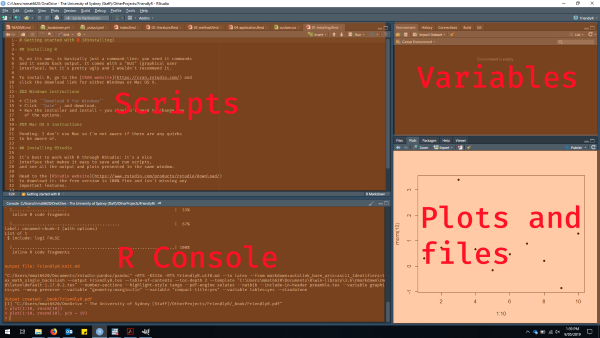
\includegraphics{Images/RStudioLayout.png}

This may look like information overload at first, but most of the time, you'll
just be looking at the \textbf{``Scripts''} section where you've written your code.

\begin{note}
\textbf{Optional:} Go to \textbf{Tools -\textgreater{} Global options
-\textgreater{} Appearance} and switch to a dark theme - it's easier on
the eyes and it looks cool.
\end{note}

You should now be able to run your first R command
by clicking in the console and typing \texttt{1\ +\ 1} and hitting
\textless Enter\textgreater:

\begin{Shaded}
\begin{Highlighting}[]
\DecValTok{1} \SpecialCharTok{+} \DecValTok{1}
\end{Highlighting}
\end{Shaded}

\begin{verbatim}
## [1] 2
\end{verbatim}

Or for something a bit more interesting, copy and paste these lines
into the console and hit \textless Enter\textgreater:

\begin{Shaded}
\begin{Highlighting}[]
\FunctionTok{plot}\NormalTok{(iris}\SpecialCharTok{$}\NormalTok{Petal.Length, iris}\SpecialCharTok{$}\NormalTok{Petal.Width, }
     \AttributeTok{xlab =} \StringTok{"Length"}\NormalTok{, }\AttributeTok{ylab =} \StringTok{"Width"}\NormalTok{, }
     \AttributeTok{main =} \StringTok{"Petals of different flower species"}\NormalTok{,}
     \AttributeTok{col =} \FunctionTok{c}\NormalTok{(}\StringTok{"green"}\NormalTok{, }\StringTok{"purple"}\NormalTok{, }\StringTok{"orange"}\NormalTok{)[iris}\SpecialCharTok{$}\NormalTok{Species],}
     \AttributeTok{pch =} \DecValTok{16}\NormalTok{)}
\end{Highlighting}
\end{Shaded}

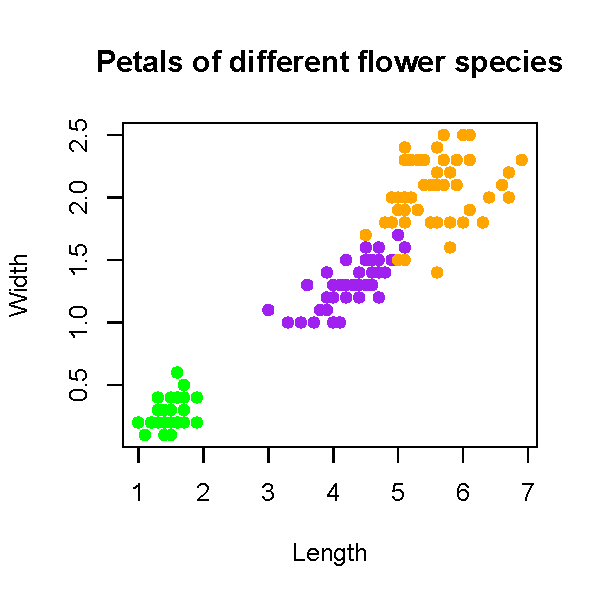
\includegraphics{Rad_files/figure-latex/first_plot-1.pdf}

\begin{note}
Don't worry if this code looks a bit complicated: some of the default
plots in R are ugly, and they need tweaking to look halfway presentable.
We'll see better ways to produce nice plots later.
\end{note}

\hypertarget{installing-your-first-packages}{%
\section{Installing your first packages}\label{installing-your-first-packages}}

A lot of the most useful tools in R come from third-party packages. Thankfully
they're easy to install, through the \texttt{install.packages()} command. Try
installing the \texttt{ggplot2} package (an excellent plotting package) to make
sure everything is working:

\begin{Shaded}
\begin{Highlighting}[]
\FunctionTok{install.packages}\NormalTok{(}\StringTok{"ggplot2"}\NormalTok{)}
\end{Highlighting}
\end{Shaded}

The install process should be automatic, and it will also install
other packages that \texttt{ggplot2} needs. Just in case, you should check
the last few lines of the output that \texttt{install.packages()} produces,
and look for messages like:

\begin{verbatim}
package ‘ggplot2’ successfully unpacked and MD5 sums checked
\end{verbatim}

\hypertarget{the-tidyverse}{%
\subsection{\texorpdfstring{The \texttt{tidyverse}}{The tidyverse}}\label{the-tidyverse}}

This is Hadley.

\begin{figure}
\centering

\includegraphics[width=\textwidth,height=2.08333in]{Images/Hadley.jpg}
\caption{Hadley Wickham}
\end{figure}

Hadley is your friend. As well as creating \texttt{ggplot2}, Hadley is the mastermind
behind the \texttt{tidyverse}, a set of R packages designed to make processing
and analysing your data easier, and to smooth out some of R's quirks.
We'll be using the \texttt{tidyverse} packages throughout this tutorial, so let's
install them now:

\begin{Shaded}
\begin{Highlighting}[]
\FunctionTok{install.packages}\NormalTok{(}\StringTok{"tidyverse"}\NormalTok{)}
\end{Highlighting}
\end{Shaded}

This will install multiple packages, but again the process should be
automatic.

\hypertarget{the-tidyverse-in-action}{%
\subsection{\texorpdfstring{The \texttt{tidyverse} in action}{The tidyverse in action}}\label{the-tidyverse-in-action}}

Now that we have some basic packages set up, let's see what they can
do for us:

\begin{Shaded}
\begin{Highlighting}[]
\CommentTok{\# Load the ggplot2 library into our R session}
\FunctionTok{library}\NormalTok{(ggplot2)}

\FunctionTok{ggplot}\NormalTok{(iris, }\FunctionTok{aes}\NormalTok{(}\AttributeTok{x =}\NormalTok{ Petal.Length, }\AttributeTok{y =}\NormalTok{ Petal.Width, }\AttributeTok{colour =}\NormalTok{ Species)) }\SpecialCharTok{+}
    \FunctionTok{geom\_point}\NormalTok{(}\AttributeTok{size =} \DecValTok{3}\NormalTok{) }\SpecialCharTok{+}
    \FunctionTok{scale\_colour\_viridis\_d}\NormalTok{() }\SpecialCharTok{+}
    \FunctionTok{labs}\NormalTok{(}\AttributeTok{title =} \StringTok{"A nicer looking plot"}\NormalTok{,}
         \AttributeTok{x =} \StringTok{"Petal length"}\NormalTok{, }\AttributeTok{y =} \StringTok{"Petal width"}\NormalTok{) }\SpecialCharTok{+}
    \FunctionTok{theme\_bw}\NormalTok{()}
\end{Highlighting}
\end{Shaded}

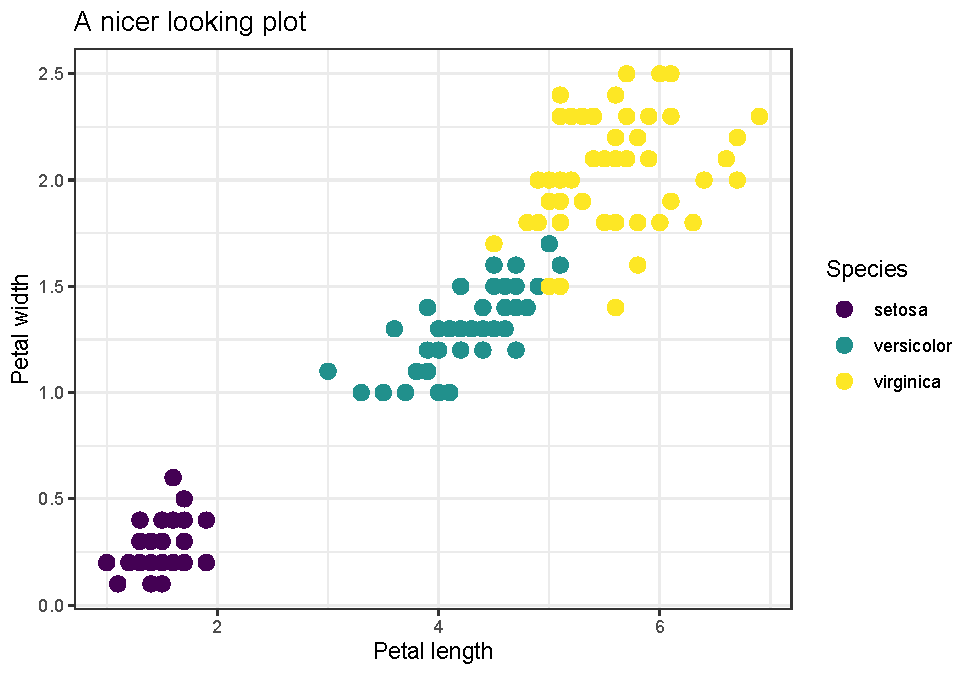
\includegraphics{Rad_files/figure-latex/iris_nicer-1.pdf}

\hypertarget{installing-other-packages}{%
\subsection{Installing other packages}\label{installing-other-packages}}

As you try out different analyses and tasks in R, you'll
come across recommendations for other packages - there are
no major drawbacks to trying them out, so feel free to install and have
a look - there are some great packages out there.

However, it's worth trying to keep the number of packages \textbf{in a single
analysis} low to avoid overlap and keep things simple (you do also get
occasional conflicts between packages where they don't play nice with each
other). If you're loading a lot of packages in your analysis
it's worth checking if you can get rid of some of them.

\hypertarget{tips-for-effective-r-programming}{%
\chapter{Tips for effective R programming}\label{tips-for-effective-r-programming}}

Before getting into actual R code, we'll start with a few notes
about how to use it most effectively. Bad coding habits can
make your R code difficult to read and understand, so hopefully
these tips will ensure you have good habits right from the start.

\hypertarget{use-rstudios-projects-feature}{%
\section{Use RStudio's ``projects'' feature}\label{use-rstudios-projects-feature}}

Every project you do in R should be set up in its own folder, through
RStudio's ``projects'' feature. To start a fresh project, go to
\textbf{File -\textgreater{} New project} and create a new folder. Reopen the project
in RStudio whenever you want to work with it.

When sending your work to other people, you can send them the whole
folder and know that they'll have access to all the required files and
scripts.

One of the main benefits is that this sets R's ``working directory'' to
the project folder by default. Any files you load or save can
just be referenced relative to that folder, so instead of:

\begin{Shaded}
\begin{Highlighting}[]
\NormalTok{data }\OtherTok{=}\NormalTok{ haven}\SpecialCharTok{::}\FunctionTok{read\_spss}\NormalTok{(}\StringTok{"R:/Project/2013/Analyses/Regressions/Data/Raw.sav"}\NormalTok{)}
\end{Highlighting}
\end{Shaded}

You can just do:

\begin{Shaded}
\begin{Highlighting}[]
\NormalTok{data }\OtherTok{=}\NormalTok{ haven}\SpecialCharTok{::}\FunctionTok{read\_spss}\NormalTok{(}\StringTok{"Data/Raw.sav"}\NormalTok{)}
\end{Highlighting}
\end{Shaded}

This will also work for anyone you send the project to, so you don't
have to worry that the file is in a different location on their machine.

\hypertarget{using-scripts}{%
\section{Using scripts}\label{using-scripts}}

It's best to put every step of your data cleaning and analysis
in a script that you save, rather than making temporary changes
in the console.

Ideally, this will mean that you (or anyone else) can run the script
from top to bottom, and get the same results every time, i.e.~they're
\textbf{reproducible}.

\hypertarget{script-layout}{%
\subsection{Script layout}\label{script-layout}}

Most R scripts I write have the same basic layout:

\begin{enumerate}
\def\labelenumi{\arabic{enumi}.}
\tightlist
\item
  Loading the libraries I'm using
\item
  Loading the data
\item
  Changing or analysing the data
\item
  Saving the results or the recoded data file
\end{enumerate}

For a larger project, it's good to create multiple different scripts for
each stage, e.g.~one file to recode the data, one to run the analyses.

When saving the recoded data, it's best to save it as a different file -
you keep the raw data, and you can recreate the recoded data
exactly by rerunning your script.

\begin{note}
R won't overwrite your data files when you change your data, unless you
specifically ask it to. When you load a file into R, it lives in R's
`short-term memory', and doesn't maintain any connection to the file on
disk. It's only when you explicitly save to a file that those changes
become permanent.
\end{note}

\hypertarget{a-tip-for-better-reproducibility}{%
\subsection{A tip for better reproducibility}\label{a-tip-for-better-reproducibility}}

By default, RStudio will save your current ``workspace'' when you
quit. While convenient, this can mean that you make one-off changes
to your data and forget to save that command in your script. Starting
with a fresh session every time you open RStudio means you'll learn
to keep every step of your analysis in your script, and you'll
know that you can get back to where you were by rerunning the script.

To disable the default setting, go to \textbf{Tools -\textgreater{} Global options..},
and in the \textbf{General} tab, and:

\begin{itemize}
\tightlist
\item
  Uncheck ``Restore .RData''
\item
  Set ``Save workspace on exit'' to ``Never''
\end{itemize}

\begin{figure}
\centering
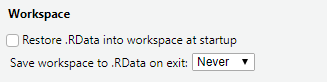
\includegraphics{Images/WorkspaceSettings.png}
\caption{RStudio's ``save workspace'' settings}
\end{figure}

\hypertarget{long-or-wide-data}{%
\section{Long or wide data}\label{long-or-wide-data}}

R works better with \textbf{long} data, whereas SPSS generally works
better with \textbf{wide} data. Roughly speaking, \textbf{long} data means:

\begin{itemize}
\tightlist
\item
  There is one ``observation'' of each participant/subject per row - e.g.~one
  survey, one session
\item
  All the measurements of the same type are in one column - so all the
  K6 scores, from multiple surveys, would be in a single \texttt{K6} column,
  with an additional \texttt{Time} or \texttt{Survey} column that identifies which
  survey they come from.
\end{itemize}

Example long data:

\begin{tabular}{r|r|l|r}
\hline
ID & Survey & Drinking & AnxietyTotal\\
\hline
1 & 1 & No & 6\\
\hline
1 & 2 & Yes & 8\\
\hline
2 & 1 & No & 5\\
\hline
2 & 2 & No & 7\\
\hline
\end{tabular}

Example wide data:

\begin{tabular}{r|l|l|r|r}
\hline
ID & Drinking\_T1 & Drinking\_T2 & AnxietyTotal\_T1 & AnxietyTotal\_T2\\
\hline
1 & No & Yes & 6 & 8\\
\hline
2 & No & No & 5 & 7\\
\hline
\end{tabular}

\hypertarget{wide-to-long}{%
\subsection{Going from wide to long}\label{wide-to-long}}

If your data is currently in wide format, you may have to \textbf{reshape}
it before working with it in R. The new \texttt{pivot\_longer} and \texttt{pivot\_wider}
functions from the \texttt{tidyr} package are good for \href{https://tidyr.tidyverse.org/dev/articles/pivot.html}{reshaping data like this}.
To go from the wide data above to a long dataset:

\begin{Shaded}
\begin{Highlighting}[]
\NormalTok{wide }\SpecialCharTok{\%\textgreater{}\%}
\NormalTok{    tidyr}\SpecialCharTok{::}\FunctionTok{pivot\_longer}\NormalTok{(}
        \AttributeTok{cols =}\NormalTok{ Drinking\_T1}\SpecialCharTok{:}\NormalTok{AnxietyTotal\_T2,}
        \AttributeTok{names\_to =} \FunctionTok{c}\NormalTok{(}\StringTok{".value"}\NormalTok{, }\StringTok{"Time"}\NormalTok{),}
        \AttributeTok{names\_sep =} \StringTok{"\_"}
\NormalTok{    )}
\end{Highlighting}
\end{Shaded}

This can get more complicated if the columns haven't been
named consistently, or have multiple pieces of info
stored in the name (e.g.~\texttt{t1\_male\_mean})

\begin{note}
At the time of writing, the \texttt{pivot} functions were still in beta,
but should be in the new \texttt{tidyr} version shortly.
\end{note}

\hypertarget{writing-readable-code}{%
\section{Writing readable code}\label{writing-readable-code}}

There are two very good reasons to try to write your code in
a clear, understandable way:

\begin{itemize}
\tightlist
\item
  Other people might need to use your code.
\item
  You might need to use your code, a few weeks/months/years
  after you've written it.
\end{itemize}

It's possible to write R code that ``works'' perfectly, and
produces all the results and output you want, but proves
very difficult to make changes to when you have to come back
to it (because a reviewer asked for one additional analysis, etc.)

\hypertarget{basic-formatting-tips}{%
\subsection{Basic formatting tips}\label{basic-formatting-tips}}

You can improve the readability of your code a lot by following
a few simple rules:

\begin{itemize}
\tightlist
\item
  Put spaces between and around variable names and operators (\texttt{=+-*/})
\item
  Break up long lines of code
\item
  Use meaningful variable names composed of 2 or 3 words (avoid abbreviations
  unless they're very common and you use them very consistently)
\end{itemize}

These rules can mean the difference between this:

\begin{Shaded}
\begin{Highlighting}[]
\NormalTok{lm1}\OtherTok{=}\FunctionTok{lm}\NormalTok{(y}\SpecialCharTok{\textasciitilde{}}\NormalTok{grp}\SpecialCharTok{+}\NormalTok{grpTime,mydf,}\AttributeTok{subset=}\NormalTok{sext1}\SpecialCharTok{==}\StringTok{"m"}\NormalTok{)}
\end{Highlighting}
\end{Shaded}

and this:

\begin{Shaded}
\begin{Highlighting}[]
\NormalTok{male\_difference }\OtherTok{=} \FunctionTok{lm}\NormalTok{(DepressionScore }\SpecialCharTok{\textasciitilde{}}\NormalTok{ Group }\SpecialCharTok{+}\NormalTok{ GroupTimeInteraction,}
                     \AttributeTok{data =}\NormalTok{ interview\_data,}
                     \AttributeTok{subset =}\NormalTok{ BaselineSex }\SpecialCharTok{==} \StringTok{"Male"}\NormalTok{)}
\end{Highlighting}
\end{Shaded}

R will treat both pieces of code exactly the same, but for any humans reading,
the nicer layout and meaningful names make it much easier to understand
what's happening, and spot any errors in syntax or intent.

\hypertarget{keeping-a-consistent-style}{%
\subsection{Keeping a consistent style}\label{keeping-a-consistent-style}}

Try to follow a consistent style for naming things, e.g.~using \texttt{snake\_case}
for all your variable names in your R code, and \texttt{TitleCase} for the
columns in your data. Either style is probably better than lowercase with
no spacing \texttt{allmashedtogether}.

It doesn't particularly matter what that style is, as long as you're
consistent. There is a \href{https://style.tidyverse.org/}{suggested style guide for the tidyverse},
but I don't follow it 100\%, I just try to be consistent within my code.

\hypertarget{writing-comments}{%
\subsection{Writing comments}\label{writing-comments}}

One of the best things you can do to make R code readable and
understandable is write comments - R ignores lines that start with
\texttt{\#} so you can write whatever you want and it won't affect
the way your code runs.

Comments that explain \emph{why} something was done are great:

\begin{Shaded}
\begin{Highlighting}[]
\CommentTok{\# Need to reverse code the score for question 3}
\NormalTok{data}\SpecialCharTok{$}\NormalTok{DepressionQ3 }\OtherTok{=} \DecValTok{4} \SpecialCharTok{{-}}\NormalTok{ data}\SpecialCharTok{$}\NormalTok{DepressionQ3}
\end{Highlighting}
\end{Shaded}

Comments that explain \emph{what} is being done are less useful. People
who already understand R code should be able to tell what is
happening just by looking at your code (especially if you're following
the other advice about writing readable code), so these comments
can be redundant:

\begin{Shaded}
\begin{Highlighting}[]
\CommentTok{\# Calculate the mean of the anxiety scores}
\NormalTok{anxiety\_mean }\OtherTok{=} \FunctionTok{mean}\NormalTok{(data}\SpecialCharTok{$}\NormalTok{AnxietyTotal)}
\end{Highlighting}
\end{Shaded}

The exception to this is when you've run into something that
was tricky to get working, and you need to explain it so other
people don't run into the same issue:

\begin{Shaded}
\begin{Highlighting}[]
\CommentTok{\# (Example only, do not run)}
\CommentTok{\# This fails to converge if we don\textquotesingle{}t set the fix\_missing option}
\NormalTok{drinking\_model }\OtherTok{=} \FunctionTok{logit\_regression}\NormalTok{(Drink }\SpecialCharTok{\textasciitilde{}}\NormalTok{ Group, }\AttributeTok{fix\_missing=}\ConstantTok{TRUE}\NormalTok{)}
\end{Highlighting}
\end{Shaded}

\hypertarget{dont-panic-dealing-with-spss-withdrawal}{%
\section{Don't panic: dealing with SPSS withdrawal}\label{dont-panic-dealing-with-spss-withdrawal}}

\hypertarget{rstudio-has-a-data-viewer}{%
\subsection{RStudio has a data viewer}\label{rstudio-has-a-data-viewer}}

As you get used to R, you should find that you get more comfortable
using the console to check on your data. You can often see
a lot of the information you need by printing the first few
rows of a dataset to the console. The \texttt{head()} function prints
the first 6 rows of a table by default, and you can select the columns that
are most relevant to what you're working on if there are too many:

\begin{Shaded}
\begin{Highlighting}[]
\FunctionTok{head}\NormalTok{(iris[, }\FunctionTok{c}\NormalTok{(}\StringTok{"Species"}\NormalTok{, }\StringTok{"Petal.Length"}\NormalTok{)])}
\end{Highlighting}
\end{Shaded}

\begin{verbatim}
##   Species Petal.Length
## 1  setosa          1.4
## 2  setosa          1.4
## 3  setosa          1.3
## 4  setosa          1.5
## 5  setosa          1.4
## 6  setosa          1.7
\end{verbatim}

However, you can also use RStudio's built-in data viewer to get a more
familiar, spreadsheet style view of your data. In the \textbf{Environment}
pane in the top-right, you can click on the name of any data you
have loaded to bring up a spreadsheet view:

\begin{figure}
\centering
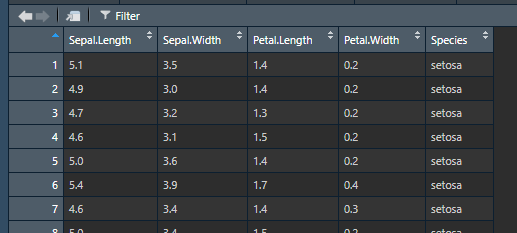
\includegraphics{Images/RstudioDataViewer.png}
\caption{Data viewer example}
\end{figure}

This also supports basic sorting and filtering so you can explore
the data more easily (you'll still need to write code using functions
like \texttt{arrange()} or \texttt{filter()} if you want to actually make
changes to the data though).

\hypertarget{r-can-read-spss-files}{%
\subsection{R can read SPSS files}\label{r-can-read-spss-files}}

The \texttt{haven} package can read (and write) SPSS data files, so you
can read in existing data:

\begin{Shaded}
\begin{Highlighting}[]
\NormalTok{survey\_one }\OtherTok{=}\NormalTok{ haven}\SpecialCharTok{::}\FunctionTok{read\_spss}\NormalTok{(}\StringTok{"Data/Survey1\_Final.sav"}\NormalTok{)}
\end{Highlighting}
\end{Shaded}

R doesn't deal with ``value labels'' in the same way as SPSS, and
\texttt{haven} tries to keep information about the SPSS value labels available.
However, it's best to just convert everything to R's way of dealing with
categorical variables, i.e.~factors, using \texttt{haven}'s \texttt{as\_factor()} function:

\begin{Shaded}
\begin{Highlighting}[]
\NormalTok{survey\_one }\OtherTok{=}\NormalTok{ haven}\SpecialCharTok{::}\FunctionTok{as\_factor}\NormalTok{(survey\_one, }\AttributeTok{levels =} \StringTok{"both"}\NormalTok{)}
\end{Highlighting}
\end{Shaded}

The \texttt{levels\ =\ "both"} option puts both the numeric value and the text label
into the factor labels, like \texttt{"{[}0{]}\ No"}, \texttt{"{[}1{]}\ Yes"}. As you get more
comfortable with R you may want to just use \texttt{levels\ =\ "labels"} so you
just get the text labels like \texttt{"No"}, \texttt{"Yes"}.

You may need to convert your data \protect\hyperlink{wide-to-long}{from wide to long}, since
SPSS prefers wide and R prefers long.

The \texttt{haven} package can also read SAS and Stata data, and there are
packages like \texttt{readxl} for Excel files. It's generally easy to read
your data into R from any format designed for tables of data.

\hypertarget{here-be-dragons-the-bad-parts-of-r}{%
\section{Here be dragons: the bad parts of R}\label{here-be-dragons-the-bad-parts-of-r}}

There are a few tools in R that tend to create more problems
than they solve. Unfortunately beginners often end up using
them (sometimes because bad tutorials recommend them). My
personal list of tools to \textbf{avoid} includes:

\begin{itemize}
\tightlist
\item
  \texttt{attach()}: This copies all the individual variables from a dataset
  into R's environment, so you can access them with just \texttt{var\_name}
  instead of \texttt{dataset\$var\_name}. The problem is:

  \begin{itemize}
  \tightlist
  \item
    You end up with \emph{a lot} of variables in your environment that are
    hard to keep track of.
  \item
    The variables can get out of sync with each other in ways
    that wouldn't be possible if they were kept in the dataset.
  \end{itemize}
\item
  \texttt{get()} and \texttt{assign()}: These allow you to look up and create variable
  names using strings, so instead of looking up \texttt{model3}, you can
  programmatically create the variable name like
  \texttt{get(paste0("model",\ model\_num))}.

  \begin{itemize}
  \tightlist
  \item
    Again, you can end up with \emph{a lot} of variables in your environment.
  \item
    People often use these when they want to run 100 different versions
    of a model (there are sometimes good reasons to do this). Instead of creating
    100 different variables called \texttt{model1}, \texttt{model2}, \ldots, \texttt{model100}, it's
    usually possible to save these in a single \texttt{list} or dataframe. Saving
    them all in a list means it's much easier to process and work
    with the results.
  \end{itemize}
\end{itemize}

\hypertarget{the-basics-of-r}{%
\chapter{The Basics of R}\label{the-basics-of-r}}

R is built around a few basic pieces - once you understand them,
it's easier to understand more complex commands, since everything
is built from the same basic foundations.

In programming terms, we can refer to the basic pieces that make
up R as \textbf{data types}.

\hypertarget{basic-data-types}{%
\section{Basic data types}\label{basic-data-types}}

\hypertarget{numbers}{%
\subsection{Numbers}\label{numbers}}

The \textbf{numeric} data type allows you to work with numbers. R can
do all the basic operations you'd expect: addition, subtraction,
multiplication and division.

At the most basic level, you can use R as a calculator by doing
standard operations like \texttt{+}, \texttt{-}, \texttt{/} (division), \texttt{*} (multiplication),
\texttt{\^{}} (power) on numeric data:

\begin{Shaded}
\begin{Highlighting}[]
\SpecialCharTok{\textgreater{}} \DecValTok{1} \SpecialCharTok{+} \DecValTok{1}
\end{Highlighting}
\end{Shaded}

\begin{verbatim}
## [1] 2
\end{verbatim}

\begin{Shaded}
\begin{Highlighting}[]
\SpecialCharTok{\textgreater{}} \FloatTok{2.5} \SpecialCharTok{*} \DecValTok{3}
\end{Highlighting}
\end{Shaded}

\begin{verbatim}
## [1] 7.5
\end{verbatim}

\begin{Shaded}
\begin{Highlighting}[]
\SpecialCharTok{\textgreater{}} \DecValTok{8}\SpecialCharTok{\^{}}\DecValTok{2}
\end{Highlighting}
\end{Shaded}

\begin{verbatim}
## [1] 64
\end{verbatim}

R also has an \textbf{integer} (whole number) data type. Integers (usually)
work exactly the same as \textbf{numeric} data, so you don't need to worry
too much about the difference for now. Integers will automatically be
converted to the more general numeric format when needed:

\begin{Shaded}
\begin{Highlighting}[]
\CommentTok{\# You can specify that data should be integers using "L"}
\NormalTok{1L }\SpecialCharTok{+}\NormalTok{ 1L}
\end{Highlighting}
\end{Shaded}

\begin{verbatim}
## [1] 2
\end{verbatim}

\begin{Shaded}
\begin{Highlighting}[]
\CommentTok{\# Automatically converts the result to numeric}
\NormalTok{3L }\SpecialCharTok{+} \FloatTok{0.1}
\end{Highlighting}
\end{Shaded}

\begin{verbatim}
## [1] 3.1
\end{verbatim}

\begin{Shaded}
\begin{Highlighting}[]
\NormalTok{5L }\SpecialCharTok{/} \DecValTok{2}
\end{Highlighting}
\end{Shaded}

\begin{verbatim}
## [1] 2.5
\end{verbatim}

\hypertarget{characters-text}{%
\subsection{Characters (text)}\label{characters-text}}

The \textbf{character} data type allows you to store and manipulate
text. Character data is created by wrapping text in either single \texttt{\textquotesingle{}} or
double \texttt{"} quotes. In programming terms, we also refer to each chunk of text
as a \textbf{string}:

\begin{Shaded}
\begin{Highlighting}[]
\StringTok{"apple"}
\end{Highlighting}
\end{Shaded}

\begin{verbatim}
## [1] "apple"
\end{verbatim}

\begin{Shaded}
\begin{Highlighting}[]
\CommentTok{\# Note: this is still just one string. All the text, including}
\CommentTok{\#   the spaces, is contained in the same chunk of text}
\FunctionTok{toupper}\NormalTok{(}\StringTok{"three bananas"}\NormalTok{)}
\end{Highlighting}
\end{Shaded}

\begin{verbatim}
## [1] "THREE BANANAS"
\end{verbatim}

\begin{Shaded}
\begin{Highlighting}[]
\CommentTok{\# Get part of a string.}
\FunctionTok{substr}\NormalTok{(}\StringTok{"carrot"}\NormalTok{, }\DecValTok{1}\NormalTok{, }\DecValTok{3}\NormalTok{)}
\end{Highlighting}
\end{Shaded}

\begin{verbatim}
## [1] "car"
\end{verbatim}

\begin{Shaded}
\begin{Highlighting}[]
\CommentTok{\# Stick multiple strings together with paste0}
\FunctionTok{paste0}\NormalTok{(}\StringTok{"for"}\NormalTok{, }\StringTok{"got"}\NormalTok{)}
\end{Highlighting}
\end{Shaded}

\begin{verbatim}
## [1] "forgot"
\end{verbatim}

\hypertarget{logical-truefalse}{%
\subsection{Logical (True/False)}\label{logical-truefalse}}

The \textbf{logical} data type is used to represent the True/False result
of a logical test or comparison. These are represented by the
special values of \texttt{TRUE} and \texttt{FALSE} (basically 1 and 0, with special labels
attached to them). To do logical comparisons, you can use syntax like:

\begin{itemize}
\tightlist
\item
  \texttt{==}: equals. Note that you need a double equal sign to compare values,
  a single equal sign does something different.
\end{itemize}

\begin{Shaded}
\begin{Highlighting}[]
\SpecialCharTok{\textgreater{}} \StringTok{"a"} \SpecialCharTok{==} \StringTok{"b"}
\end{Highlighting}
\end{Shaded}

\begin{verbatim}
## [1] FALSE
\end{verbatim}

\begin{itemize}
\tightlist
\item
  \texttt{\textless{}}, \texttt{\textgreater{}}: less than, greater than
\end{itemize}

\begin{Shaded}
\begin{Highlighting}[]
\DecValTok{3} \SpecialCharTok{\textless{}} \DecValTok{4}
\end{Highlighting}
\end{Shaded}

\begin{verbatim}
## [1] TRUE
\end{verbatim}

\begin{itemize}
\tightlist
\item
  \texttt{\textless{}=}, \texttt{\textgreater{}=}: less than or equal to, greater than or equal to
\end{itemize}

\begin{Shaded}
\begin{Highlighting}[]
\DecValTok{10} \SpecialCharTok{\textgreater{}=} \DecValTok{10}
\end{Highlighting}
\end{Shaded}

\begin{verbatim}
## [1] TRUE
\end{verbatim}

\begin{itemize}
\tightlist
\item
  \texttt{!=}: not equal to
\end{itemize}

\begin{Shaded}
\begin{Highlighting}[]
\StringTok{"hello"} \SpecialCharTok{!=} \StringTok{"world"}
\end{Highlighting}
\end{Shaded}

\begin{verbatim}
## [1] TRUE
\end{verbatim}

\begin{itemize}
\tightlist
\item
  \texttt{!}: not, which reverses the result of another logical test:
\end{itemize}

\begin{Shaded}
\begin{Highlighting}[]
\SpecialCharTok{\textgreater{}} \SpecialCharTok{!}\NormalTok{ (}\DecValTok{5} \SpecialCharTok{\textgreater{}} \DecValTok{3}\NormalTok{)}
\end{Highlighting}
\end{Shaded}

\begin{verbatim}
## [1] FALSE
\end{verbatim}

\hypertarget{combining-logicals-and-and-or}{%
\subsubsection{Combining logicals: AND and OR}\label{combining-logicals-and-and-or}}

More complex logical tests can be conducted by combining multiple tests
with the \textbf{and} \texttt{\&} and \textbf{or} \texttt{\textbar{}} operators.

\texttt{\&} takes two logicals, e.g.~\texttt{a\ \&\ b}, and returns \texttt{TRUE} if both \texttt{a} \emph{and} \texttt{b}
are \texttt{TRUE}, and \texttt{FALSE} otherwise.

\begin{Shaded}
\begin{Highlighting}[]
\CommentTok{\# Both conditions are true: TRUE \& TRUE is TRUE}
\NormalTok{(}\DecValTok{2} \SpecialCharTok{\textgreater{}} \DecValTok{1}\NormalTok{) }\SpecialCharTok{\&}\NormalTok{ (}\StringTok{"a"} \SpecialCharTok{==} \StringTok{"a"}\NormalTok{)}
\end{Highlighting}
\end{Shaded}

\begin{verbatim}
## [1] TRUE
\end{verbatim}

\begin{Shaded}
\begin{Highlighting}[]
\CommentTok{\# Only one condition is true: TRUE \& FALSE is FALSE}
\NormalTok{(}\DecValTok{3} \SpecialCharTok{\textgreater{}=} \DecValTok{3}\NormalTok{) }\SpecialCharTok{\&}\NormalTok{ (}\StringTok{"b"} \SpecialCharTok{==} \StringTok{"a"}\NormalTok{)}
\end{Highlighting}
\end{Shaded}

\begin{verbatim}
## [1] FALSE
\end{verbatim}

\texttt{a\ \textbar{}\ b} returns \texttt{TRUE} if either \texttt{a} \emph{or} \texttt{b} is \texttt{TRUE}

\begin{Shaded}
\begin{Highlighting}[]
\CommentTok{\# FALSE | TRUE is TRUE}
\NormalTok{(}\DecValTok{1} \SpecialCharTok{\textgreater{}} \DecValTok{2}\NormalTok{) }\SpecialCharTok{|}\NormalTok{ (}\StringTok{"a"} \SpecialCharTok{==} \StringTok{"a"}\NormalTok{)}
\end{Highlighting}
\end{Shaded}

\begin{verbatim}
## [1] TRUE
\end{verbatim}

\begin{Shaded}
\begin{Highlighting}[]
\CommentTok{\# FALSE | FALSE is FALSE}
\NormalTok{(}\DecValTok{1} \SpecialCharTok{\textgreater{}} \DecValTok{2}\NormalTok{) }\SpecialCharTok{|}\NormalTok{ (}\StringTok{"a"} \SpecialCharTok{==} \StringTok{"b"}\NormalTok{)}
\end{Highlighting}
\end{Shaded}

\begin{verbatim}
## [1] FALSE
\end{verbatim}

It's best to wrap each individual test in parentheses \texttt{()} to make the logic clear.

\hypertarget{converting-between-types}{%
\section{Converting between types}\label{converting-between-types}}

Occasionally your data will be read in from a file as the wrong type.
You might be able to fix this by changing the way you read in the file,
but otherwise you should \textbf{convert} the data to the type that makes
the most sense (you might have to clean up some invalid values first).

Functions like \texttt{as.character()}, \texttt{as.numeric()} and \texttt{as.logical()} will
convert data to the relevant type. Probably the most common type conversion
you'll have to do is when \texttt{numeric} data gets treated as text and is stored
as \texttt{character}. Numeric operations like addition won't work until you fix
this:

\begin{Shaded}
\begin{Highlighting}[]
\StringTok{"1"} \SpecialCharTok{+} \DecValTok{1}
\end{Highlighting}
\end{Shaded}

\begin{verbatim}
## Error in "1" + 1: non-numeric argument to binary operator
\end{verbatim}

\begin{Shaded}
\begin{Highlighting}[]
\NormalTok{one\_fixed }\OtherTok{=} \FunctionTok{as.numeric}\NormalTok{(}\StringTok{"1"}\NormalTok{)}
\NormalTok{one\_fixed }\SpecialCharTok{+} \DecValTok{1}
\end{Highlighting}
\end{Shaded}

\begin{verbatim}
## [1] 2
\end{verbatim}

\hypertarget{variables-storing-results}{%
\section{Variables: Storing Results}\label{variables-storing-results}}

The results of calculations in R can be stored in \textbf{variables}: you
give a name to the results, and then when you want to look at, use
or change those results later, you access them using the same name.

You \textbf{assign} a value to a variable using either \texttt{=} or \texttt{\textless{}-} (these
are mostly equivalent, don't worry too much about the difference), putting
the variable name on the left hand side and the value on the right.

\begin{Shaded}
\begin{Highlighting}[]
\NormalTok{scale\_total }\OtherTok{=} \DecValTok{3} \SpecialCharTok{+} \DecValTok{8} \SpecialCharTok{+} \DecValTok{5} \SpecialCharTok{+} \DecValTok{2} \SpecialCharTok{+} \DecValTok{4}
\CommentTok{\# Accessing saved results}
\NormalTok{scale\_total}
\end{Highlighting}
\end{Shaded}

\begin{verbatim}
## [1] 22
\end{verbatim}

\begin{Shaded}
\begin{Highlighting}[]
\CommentTok{\# Using saved results in another calculation}
\NormalTok{severe\_disorder }\OtherTok{=}\NormalTok{ scale\_total }\SpecialCharTok{\textgreater{}=} \DecValTok{15}
\NormalTok{severe\_disorder}
\end{Highlighting}
\end{Shaded}

\begin{verbatim}
## [1] TRUE
\end{verbatim}

\begin{Shaded}
\begin{Highlighting}[]
\CommentTok{\# Changing a variable: this will overwrite the old value with the}
\CommentTok{\#   new one, the old value won\textquotesingle{}t be available unless you\textquotesingle{}ve}
\CommentTok{\#   stored it somewhere else}
\NormalTok{scale\_total }\OtherTok{=}\NormalTok{ scale\_total }\SpecialCharTok{+} \DecValTok{2}
\NormalTok{scale\_total}
\end{Highlighting}
\end{Shaded}

\begin{verbatim}
## [1] 24
\end{verbatim}

\textbf{When you assign a variable, you're asking R to remember some data so you can
use it later.} Understanding that simple
principle will take you a long way in R programming.

The \textbf{expression} on the right hand side might be long and complex,
but as long as it's valid R code that creates a single value,
all you're doing is creating a single value and assigning it to
a name, just like in the simple examples above.

Variable names in R should start with a letter (\texttt{a-zA-Z}), and
can contain letters, numbers, underscores \texttt{\_} and periods \texttt{.}, so
\texttt{model3}, \texttt{get.scores}, \texttt{ANX\_total} are all valid variable names.

\hypertarget{copying-variables}{%
\subsection{Copying Variables}\label{copying-variables}}

If you assign an existing value to a new variable, it will
create a copy. If you change one copy, the other will
stay as it was:

\begin{Shaded}
\begin{Highlighting}[]
\NormalTok{a }\OtherTok{=} \DecValTok{3}
\CommentTok{\# b is a copy of a}
\NormalTok{b }\OtherTok{=}\NormalTok{ a}
\NormalTok{b }\OtherTok{=}\NormalTok{ b }\SpecialCharTok{+} \DecValTok{2}
\CommentTok{\# We didn\textquotesingle{}t change a}
\NormalTok{a}
\end{Highlighting}
\end{Shaded}

\begin{verbatim}
## [1] 3
\end{verbatim}

\begin{Shaded}
\begin{Highlighting}[]
\CommentTok{\# We only changed the copy}
\NormalTok{b}
\end{Highlighting}
\end{Shaded}

\begin{verbatim}
## [1] 5
\end{verbatim}

This can be useful if you want to test out some changes to your data, or create
multiple different subsets of the same data.

\hypertarget{vectors}{%
\section{Vectors}\label{vectors}}

All the data-types discussed above can be stored in \textbf{vectors}\footnote{Actually, most things in R are vectors, even when they look like
  single values. Even the single elements shown above, like \texttt{3}, are just
  vectors with a length of 1.}, which
are sequences with multiple elements of the same type. Vectors can be
created using the \texttt{c()} function to put together multiple elements.

\begin{Shaded}
\begin{Highlighting}[]
\SpecialCharTok{\textgreater{}} \FunctionTok{c}\NormalTok{(}\DecValTok{1}\NormalTok{, }\DecValTok{2}\NormalTok{, }\DecValTok{3}\NormalTok{, }\DecValTok{10}\NormalTok{)}
\end{Highlighting}
\end{Shaded}

\begin{verbatim}
## [1]  1  2  3 10
\end{verbatim}

The number of elements in a vector is the \textbf{length}:

\begin{Shaded}
\begin{Highlighting}[]
\SpecialCharTok{\textgreater{}} \FunctionTok{length}\NormalTok{(}\FunctionTok{c}\NormalTok{(}\StringTok{"a"}\NormalTok{, }\StringTok{"b"}\NormalTok{, }\StringTok{"c"}\NormalTok{))}
\end{Highlighting}
\end{Shaded}

\begin{verbatim}
## [1] 3
\end{verbatim}

\hypertarget{calculating-with-vectors}{%
\subsection{Calculating with vectors}\label{calculating-with-vectors}}

R automatically applies most calculations and operations to every element
of a vector at the same time, so you work with vectors the same way
you would single values\footnote{In other programming languages, you might have to manually
  apply the operation to each element of the sequence, using something
  like a for loop.}.

Adding, multipying, or comparing a single value with a vector automatically
adds, multiplies or compares the single value to every element of the vector.
The result is a new vector with the same length:

\begin{Shaded}
\begin{Highlighting}[]
\SpecialCharTok{\textgreater{}} \DecValTok{1} \SpecialCharTok{+} \FunctionTok{c}\NormalTok{(}\DecValTok{1}\NormalTok{, }\DecValTok{2}\NormalTok{, }\DecValTok{3}\NormalTok{)}
\end{Highlighting}
\end{Shaded}

\begin{verbatim}
## [1] 2 3 4
\end{verbatim}

\begin{Shaded}
\begin{Highlighting}[]
\SpecialCharTok{\textgreater{}} \DecValTok{3} \SpecialCharTok{*} \FunctionTok{c}\NormalTok{(}\DecValTok{10}\NormalTok{, }\DecValTok{20}\NormalTok{, }\DecValTok{30}\NormalTok{)}
\end{Highlighting}
\end{Shaded}

\begin{verbatim}
## [1] 30 60 90
\end{verbatim}

\begin{Shaded}
\begin{Highlighting}[]
\SpecialCharTok{\textgreater{}} \StringTok{"banana"} \SpecialCharTok{==} \FunctionTok{c}\NormalTok{(}\StringTok{"apple"}\NormalTok{, }\StringTok{"banana"}\NormalTok{, }\StringTok{"carrot"}\NormalTok{)}
\end{Highlighting}
\end{Shaded}

\begin{verbatim}
## [1] FALSE  TRUE FALSE
\end{verbatim}

When you work with two vectors of the same length, R automatically
matches up the first element of one vector with the first element
of the other, the second element with the second element, and so on:

\begin{Shaded}
\begin{Highlighting}[]
\SpecialCharTok{\textgreater{}} \FunctionTok{c}\NormalTok{(}\DecValTok{1}\NormalTok{, }\DecValTok{2}\NormalTok{, }\DecValTok{3}\NormalTok{) }\SpecialCharTok{+} \FunctionTok{c}\NormalTok{(}\DecValTok{10}\NormalTok{, }\DecValTok{20}\NormalTok{, }\DecValTok{30}\NormalTok{)}
\end{Highlighting}
\end{Shaded}

\begin{verbatim}
## [1] 11 22 33
\end{verbatim}

\begin{Shaded}
\begin{Highlighting}[]
\SpecialCharTok{\textgreater{}} \FunctionTok{c}\NormalTok{(}\StringTok{"a"}\NormalTok{, }\StringTok{"b"}\NormalTok{, }\StringTok{"c"}\NormalTok{) }\SpecialCharTok{==} \FunctionTok{c}\NormalTok{(}\StringTok{"a"}\NormalTok{, }\StringTok{"x"}\NormalTok{, }\StringTok{"c"}\NormalTok{)}
\end{Highlighting}
\end{Shaded}

\begin{verbatim}
## [1]  TRUE FALSE  TRUE
\end{verbatim}

\textbf{NB: not recommended!} It's possible to do some tricks with
vectors of different lengths, but it's generally not needed. Usually,
you'll either have a single value you want to work with, or vectors
that are all the same length.

\begin{Shaded}
\begin{Highlighting}[]
\SpecialCharTok{\textgreater{}} \CommentTok{\# "Clever", but not recommended}
\ErrorTok{\textgreater{}} \FunctionTok{c}\NormalTok{(}\DecValTok{0}\NormalTok{, }\DecValTok{1}\NormalTok{) }\SpecialCharTok{*} \FunctionTok{c}\NormalTok{(}\DecValTok{1}\NormalTok{, }\DecValTok{2}\NormalTok{, }\DecValTok{3}\NormalTok{, }\DecValTok{4}\NormalTok{, }\DecValTok{5}\NormalTok{, }\DecValTok{6}\NormalTok{, }\DecValTok{7}\NormalTok{, }\DecValTok{8}\NormalTok{)}
\end{Highlighting}
\end{Shaded}

\begin{verbatim}
## [1] 0 2 0 4 0 6 0 8
\end{verbatim}

Most of the time, trying to work with two vectors of different lengths
will just produce a warning or an error that lets you know something
is wrong:

\begin{Shaded}
\begin{Highlighting}[]
\SpecialCharTok{\textgreater{}} \FunctionTok{c}\NormalTok{(}\DecValTok{5}\NormalTok{, }\DecValTok{6}\NormalTok{) }\SpecialCharTok{*} \FunctionTok{c}\NormalTok{(}\DecValTok{3}\NormalTok{, }\DecValTok{8}\NormalTok{, }\DecValTok{4}\NormalTok{)}
\end{Highlighting}
\end{Shaded}

\begin{verbatim}
## Warning in c(5, 6) * c(3, 8, 4): longer object length is not a multiple of
## shorter object length
\end{verbatim}

\begin{verbatim}
## [1] 15 48 20
\end{verbatim}

\hypertarget{r-is-built-around-vectors}{%
\subsubsection{R is built around vectors}\label{r-is-built-around-vectors}}

The details above are relevant when you need to do custom calculations
manually. But of course, R already has plenty of built-in commands,
and these are all designed to work with vectors. A lot of the time,
you'll just be feeding vectors into existing commands:

\begin{Shaded}
\begin{Highlighting}[]
\SpecialCharTok{\textgreater{}} \FunctionTok{sum}\NormalTok{(}\FunctionTok{c}\NormalTok{(}\DecValTok{1}\NormalTok{, }\DecValTok{2}\NormalTok{, }\DecValTok{3}\NormalTok{))}
\end{Highlighting}
\end{Shaded}

\begin{verbatim}
## [1] 6
\end{verbatim}

\begin{Shaded}
\begin{Highlighting}[]
\SpecialCharTok{\textgreater{}} \FunctionTok{mean}\NormalTok{(}\FunctionTok{c}\NormalTok{(}\DecValTok{10}\NormalTok{, }\DecValTok{12}\NormalTok{, }\DecValTok{16}\NormalTok{, }\DecValTok{18}\NormalTok{))}
\end{Highlighting}
\end{Shaded}

\begin{verbatim}
## [1] 14
\end{verbatim}

\begin{Shaded}
\begin{Highlighting}[]
\SpecialCharTok{\textgreater{}} \FunctionTok{t.test}\NormalTok{(}\FunctionTok{c}\NormalTok{(}\DecValTok{1}\NormalTok{, }\DecValTok{2}\NormalTok{, }\DecValTok{3}\NormalTok{, }\DecValTok{4}\NormalTok{), }\FunctionTok{c}\NormalTok{(}\DecValTok{1}\NormalTok{, }\DecValTok{2}\NormalTok{, }\DecValTok{3}\NormalTok{, }\DecValTok{5}\NormalTok{))}
\end{Highlighting}
\end{Shaded}

\begin{verbatim}
## 
##  Welch Two Sample t-test
## 
## data:  c(1, 2, 3, 4) and c(1, 2, 3, 5)
## t = -0.23355, df = 5.5846, p-value = 0.8237
## alternative hypothesis: true difference in means is not equal to 0
## 95 percent confidence interval:
##  -2.917221  2.417221
## sample estimates:
## mean of x mean of y 
##      2.50      2.75
\end{verbatim}

\hypertarget{missing-values}{%
\subsection{Missing values}\label{missing-values}}

All types of vectors allow for missing data, through the special \texttt{NA}
value.

\begin{Shaded}
\begin{Highlighting}[]
\FunctionTok{c}\NormalTok{(}\DecValTok{29}\NormalTok{, }\ConstantTok{NA}\NormalTok{, }\DecValTok{14}\NormalTok{)}
\end{Highlighting}
\end{Shaded}

\begin{verbatim}
## [1] 29 NA 14
\end{verbatim}

Generally, \texttt{NA} values will stay \texttt{NA} when you try to calculate
with the vector.

\begin{Shaded}
\begin{Highlighting}[]
\FunctionTok{c}\NormalTok{(}\DecValTok{29}\NormalTok{, }\ConstantTok{NA}\NormalTok{, }\DecValTok{14}\NormalTok{) }\SpecialCharTok{*} \DecValTok{2}
\end{Highlighting}
\end{Shaded}

\begin{verbatim}
## [1] 58 NA 28
\end{verbatim}

\begin{Shaded}
\begin{Highlighting}[]
\FunctionTok{toupper}\NormalTok{(}\FunctionTok{c}\NormalTok{(}\StringTok{"a"}\NormalTok{, }\ConstantTok{NA}\NormalTok{, }\StringTok{"c"}\NormalTok{))}
\end{Highlighting}
\end{Shaded}

\begin{verbatim}
## [1] "A" NA  "C"
\end{verbatim}

\begin{Shaded}
\begin{Highlighting}[]
\CommentTok{\# Missing values on either side of the sum will produce}
\CommentTok{\#   missing values in the result}
\FunctionTok{c}\NormalTok{(}\DecValTok{1}\NormalTok{, }\ConstantTok{NA}\NormalTok{, }\DecValTok{3}\NormalTok{) }\SpecialCharTok{+} \FunctionTok{c}\NormalTok{(}\DecValTok{4}\NormalTok{, }\DecValTok{5}\NormalTok{, }\ConstantTok{NA}\NormalTok{)}
\end{Highlighting}
\end{Shaded}

\begin{verbatim}
## [1]  5 NA NA
\end{verbatim}

The \texttt{is.na()} function can test which values are missing:

\begin{Shaded}
\begin{Highlighting}[]
\FunctionTok{is.na}\NormalTok{(}\FunctionTok{c}\NormalTok{(}\DecValTok{1}\NormalTok{, }\ConstantTok{NA}\NormalTok{, }\DecValTok{3}\NormalTok{))}
\end{Highlighting}
\end{Shaded}

\begin{verbatim}
## [1] FALSE  TRUE FALSE
\end{verbatim}

Functions like \texttt{sum()} and \texttt{mean()} will produce a missing
result by default if \emph{any} values in the input are missing. Use the
\texttt{na.rm\ =\ TRUE} option (short for ``\texttt{NA} remove'') to ignore the missing values
and just use the values that are available:

\begin{Shaded}
\begin{Highlighting}[]
\FunctionTok{mean}\NormalTok{(}\FunctionTok{c}\NormalTok{(}\DecValTok{1}\NormalTok{, }\DecValTok{3}\NormalTok{, }\ConstantTok{NA}\NormalTok{, }\DecValTok{7}\NormalTok{, }\DecValTok{9}\NormalTok{))}
\end{Highlighting}
\end{Shaded}

\begin{verbatim}
## [1] NA
\end{verbatim}

\begin{Shaded}
\begin{Highlighting}[]
\FunctionTok{mean}\NormalTok{(}\FunctionTok{c}\NormalTok{(}\DecValTok{1}\NormalTok{, }\DecValTok{3}\NormalTok{, }\ConstantTok{NA}\NormalTok{, }\DecValTok{7}\NormalTok{, }\DecValTok{9}\NormalTok{), }\AttributeTok{na.rm =} \ConstantTok{TRUE}\NormalTok{)}
\end{Highlighting}
\end{Shaded}

\begin{verbatim}
## [1] 5
\end{verbatim}

Other functions in R will automatically remove missing values, but
will usually warn you when they do. It's always good to check
how missing values are being treated, whatever tool you're using.

\hypertarget{indexing-accessing-parts-of-vectors}{%
\subsection{Indexing: accessing parts of vectors}\label{indexing-accessing-parts-of-vectors}}

To access parts of a vector, use square brackets \texttt{{[}{]}} after the vector
and use integers to specify which parts you want to extract. E.g. to
extract the second element:

\begin{Shaded}
\begin{Highlighting}[]
\FunctionTok{c}\NormalTok{(}\StringTok{"a"}\NormalTok{, }\StringTok{"b"}\NormalTok{, }\StringTok{"c"}\NormalTok{, }\StringTok{"d"}\NormalTok{)[}\DecValTok{2}\NormalTok{]}
\end{Highlighting}
\end{Shaded}

\begin{verbatim}
## [1] "b"
\end{verbatim}

This is known as \textbf{indexing}. Here, 2 is the \textbf{index}.

To extract multiple elements, you can use a vector as the index. R
returns a new vector, containing the elements that match up to the index.

\begin{Shaded}
\begin{Highlighting}[]
\FunctionTok{c}\NormalTok{(}\StringTok{"a"}\NormalTok{, }\StringTok{"b"}\NormalTok{, }\StringTok{"c"}\NormalTok{, }\StringTok{"d"}\NormalTok{)[}\FunctionTok{c}\NormalTok{(}\DecValTok{2}\NormalTok{, }\DecValTok{3}\NormalTok{, }\DecValTok{4}\NormalTok{)]}
\end{Highlighting}
\end{Shaded}

\begin{verbatim}
## [1] "b" "c" "d"
\end{verbatim}

\begin{Shaded}
\begin{Highlighting}[]
\CommentTok{\# This is a handy shortcut that does the same thing}
\FunctionTok{c}\NormalTok{(}\StringTok{"a"}\NormalTok{, }\StringTok{"b"}\NormalTok{, }\StringTok{"c"}\NormalTok{, }\StringTok{"d"}\NormalTok{)[}\DecValTok{2}\SpecialCharTok{:}\DecValTok{4}\NormalTok{]}
\end{Highlighting}
\end{Shaded}

\begin{verbatim}
## [1] "b" "c" "d"
\end{verbatim}

The index can include any number between 1 and the length
of the vector, in any order. You can also access the same
element multiple times:

\begin{Shaded}
\begin{Highlighting}[]
\FunctionTok{c}\NormalTok{(}\StringTok{"a"}\NormalTok{, }\StringTok{"b"}\NormalTok{, }\StringTok{"c"}\NormalTok{, }\StringTok{"d"}\NormalTok{)[}\FunctionTok{c}\NormalTok{(}\DecValTok{4}\NormalTok{, }\DecValTok{1}\NormalTok{, }\DecValTok{2}\NormalTok{, }\DecValTok{3}\NormalTok{, }\DecValTok{1}\NormalTok{, }\DecValTok{2}\NormalTok{)]}
\end{Highlighting}
\end{Shaded}

\begin{verbatim}
## [1] "d" "a" "b" "c" "a" "b"
\end{verbatim}

\hypertarget{logical-indexing-filtering-your-data-based-on-conditions}{%
\subsection{Logical indexing: filtering your data based on conditions}\label{logical-indexing-filtering-your-data-based-on-conditions}}

One of the most powerful tools in R is the ability to
access the subset of your data that meets a condition.
If you use a \textbf{logical} vector as the index for
your vector, R returns a new vector containing just the elements
where the index was \texttt{TRUE}:

\begin{Shaded}
\begin{Highlighting}[]
\FunctionTok{c}\NormalTok{(}\DecValTok{20}\NormalTok{, }\DecValTok{10}\NormalTok{, }\DecValTok{30}\NormalTok{)[}\FunctionTok{c}\NormalTok{(}\ConstantTok{TRUE}\NormalTok{, }\ConstantTok{FALSE}\NormalTok{, }\ConstantTok{TRUE}\NormalTok{)]}
\end{Highlighting}
\end{Shaded}

\begin{verbatim}
## [1] 20 30
\end{verbatim}

This means you can filter the vector using the results of a logical
test:

\begin{Shaded}
\begin{Highlighting}[]
\NormalTok{x }\OtherTok{=} \FunctionTok{c}\NormalTok{(}\DecValTok{20}\NormalTok{, }\DecValTok{10}\NormalTok{, }\DecValTok{30}\NormalTok{)}
\CommentTok{\# Same results as above}
\NormalTok{x[x }\SpecialCharTok{\textgreater{}=} \DecValTok{20}\NormalTok{]}
\end{Highlighting}
\end{Shaded}

\begin{verbatim}
## [1] 20 30
\end{verbatim}

This works because the result of \texttt{x\ \textgreater{}=\ 20} is a logical vector
\texttt{c(TRUE,\ FALSE,\ TRUE)}, which works just like it did above. If you're having
trouble understanding a complex R expression, you can often pull out the
individual parts and test them separately to see how they work.

This kind of logical subsetting is particularly useful
once you start testing based on other vectors:

\begin{Shaded}
\begin{Highlighting}[]
\NormalTok{group }\OtherTok{=} \FunctionTok{c}\NormalTok{(}\StringTok{"Control"}\NormalTok{, }\StringTok{"Treatment"}\NormalTok{, }\StringTok{"Treatment"}\NormalTok{, }\StringTok{"Control"}\NormalTok{)}
\NormalTok{score }\OtherTok{=} \FunctionTok{c}\NormalTok{(}\DecValTok{6}\NormalTok{, }\DecValTok{5}\NormalTok{, }\DecValTok{7}\NormalTok{, }\DecValTok{4}\NormalTok{)}
\NormalTok{score[group }\SpecialCharTok{==} \StringTok{"Treatment"}\NormalTok{]}
\end{Highlighting}
\end{Shaded}

\begin{verbatim}
## [1] 5 7
\end{verbatim}

\hypertarget{changing-vectors}{%
\subsection{Changing vectors}\label{changing-vectors}}

To change part of a vector, you can index the vector on the left-hand
side of the \texttt{=}/\texttt{\textless{}-} symbol and put the replacement on the right-hand
side. You just need to make sure the replacement is either:

\begin{itemize}
\tightlist
\item
  A single value, or
\item
  The same length as the part you're replacing.
\end{itemize}

\begin{Shaded}
\begin{Highlighting}[]
\NormalTok{x }\OtherTok{=} \FunctionTok{c}\NormalTok{(}\DecValTok{11}\NormalTok{, }\DecValTok{15}\NormalTok{, }\DecValTok{12}\NormalTok{, }\DecValTok{13}\NormalTok{, }\DecValTok{18}\NormalTok{)}
\CommentTok{\# Replace a single element}
\NormalTok{x[}\DecValTok{4}\NormalTok{] }\OtherTok{=} \DecValTok{44}
\NormalTok{x}
\end{Highlighting}
\end{Shaded}

\begin{verbatim}
## [1] 11 15 12 44 18
\end{verbatim}

\begin{Shaded}
\begin{Highlighting}[]
\CommentTok{\# Replace multiple elements}
\NormalTok{x[}\DecValTok{2}\SpecialCharTok{:}\DecValTok{4}\NormalTok{] }\OtherTok{=} \FunctionTok{c}\NormalTok{(}\DecValTok{6}\NormalTok{, }\DecValTok{7}\NormalTok{, }\DecValTok{8}\NormalTok{)}
\NormalTok{x}
\end{Highlighting}
\end{Shaded}

\begin{verbatim}
## [1] 11  6  7  8 18
\end{verbatim}

\begin{Shaded}
\begin{Highlighting}[]
\CommentTok{\# Replace based on a test}
\NormalTok{x }\OtherTok{=} \FunctionTok{c}\NormalTok{(}\DecValTok{11}\NormalTok{, }\DecValTok{15}\NormalTok{, }\DecValTok{12}\NormalTok{, }\DecValTok{13}\NormalTok{, }\DecValTok{18}\NormalTok{)}
\NormalTok{x[x }\SpecialCharTok{\textgreater{}} \DecValTok{14}\NormalTok{] }\OtherTok{=} \DecValTok{0}
\NormalTok{x}
\end{Highlighting}
\end{Shaded}

\begin{verbatim}
## [1] 11  0 12 13  0
\end{verbatim}

\hypertarget{dataframes-and-more}{%
\chapter{Dataframes and More}\label{dataframes-and-more}}

Once you understand the basics of R's data types, some of the more
advanced features of R start to make sense. Below, we'll cover
some of these more advanced features. In particular, we'll discuss
\textbf{data frames}, which are used to store and analyse multiple
rows and columns of data bundled together in a table.

\hypertarget{factors-categorical-data}{%
\section{Factors (categorical data)}\label{factors-categorical-data}}

\textbf{Factors} are how R represents categorical data. They
have a fixed number of \textbf{levels}, that are set up when you first
create a factor vector:

\begin{Shaded}
\begin{Highlighting}[]
\NormalTok{severity }\OtherTok{=} \FunctionTok{sample}\NormalTok{(}\FunctionTok{c}\NormalTok{(}\StringTok{"Moderate"}\NormalTok{, }\StringTok{"Severe"}\NormalTok{), }\DecValTok{10}\NormalTok{, }\AttributeTok{replace=}\ConstantTok{TRUE}\NormalTok{)}
\CommentTok{\# Setting \textquotesingle{}levels\textquotesingle{} also sets the order of the levels}
\NormalTok{sev\_factor }\OtherTok{=} \FunctionTok{factor}\NormalTok{(severity, }\AttributeTok{levels =} \FunctionTok{c}\NormalTok{(}\StringTok{"Moderate"}\NormalTok{, }\StringTok{"Severe"}\NormalTok{))}
\NormalTok{sev\_factor}
\end{Highlighting}
\end{Shaded}

\begin{verbatim}
##  [1] Moderate Severe   Moderate Severe   Severe   Moderate Moderate Moderate
##  [9] Moderate Moderate
## Levels: Moderate Severe
\end{verbatim}

When you're testing a factor, you use the \textbf{label} to test it:

\begin{Shaded}
\begin{Highlighting}[]
\NormalTok{sev\_factor }\SpecialCharTok{==} \StringTok{"Moderate"}
\end{Highlighting}
\end{Shaded}

\begin{verbatim}
##  [1]  TRUE FALSE  TRUE FALSE FALSE  TRUE  TRUE  TRUE  TRUE  TRUE
\end{verbatim}

Factors can only contain data that matches their levels,
and will produce a warning if you try to add something else:

\begin{Shaded}
\begin{Highlighting}[]
\CommentTok{\# Not one of the levels that was set up when the factor was}
\CommentTok{\#   created:}
\NormalTok{sev\_factor[}\DecValTok{1}\NormalTok{] }\OtherTok{=} \StringTok{"Mild"}
\end{Highlighting}
\end{Shaded}

\begin{verbatim}
## Warning in `[<-.factor`(`*tmp*`, 1, value = "Mild"): invalid factor level, NA
## generated
\end{verbatim}

\begin{Shaded}
\begin{Highlighting}[]
\NormalTok{sev\_factor}
\end{Highlighting}
\end{Shaded}

\begin{verbatim}
##  [1] <NA>     Severe   Moderate Severe   Severe   Moderate Moderate Moderate
##  [9] Moderate Moderate
## Levels: Moderate Severe
\end{verbatim}

\hypertarget{lists}{%
\section{Lists}\label{lists}}

\textbf{Lists} in R can be used to store multiple different types of
data together. Unlike vectors, each element of a list can be a
different type:

\begin{Shaded}
\begin{Highlighting}[]
\FunctionTok{list}\NormalTok{(}\DecValTok{1}\NormalTok{, }\ConstantTok{FALSE}\NormalTok{, }\StringTok{"c"}\NormalTok{)}
\end{Highlighting}
\end{Shaded}

\begin{verbatim}
## [[1]]
## [1] 1
## 
## [[2]]
## [1] FALSE
## 
## [[3]]
## [1] "c"
\end{verbatim}

One of the most useful features of lists is you can give
each element a name, and then access the data later using
the name. This means you don't have to remember things like
``in these results, the 1st element is the mean and the 2nd is the
variance''.

To access the named elements of a list, use a dollar sign
\texttt{\$} or double square brackets \texttt{{[}{[}{]}{]}}:

\begin{Shaded}
\begin{Highlighting}[]
\NormalTok{results }\OtherTok{=} \FunctionTok{list}\NormalTok{(}\AttributeTok{mean =} \FloatTok{4.83}\NormalTok{, }\AttributeTok{variance =} \FloatTok{1.09}\NormalTok{)}
\NormalTok{results}\SpecialCharTok{$}\NormalTok{mean}
\end{Highlighting}
\end{Shaded}

\begin{verbatim}
## [1] 4.83
\end{verbatim}

\begin{Shaded}
\begin{Highlighting}[]
\NormalTok{results[[}\StringTok{"variance"}\NormalTok{]]}
\end{Highlighting}
\end{Shaded}

\begin{verbatim}
## [1] 1.09
\end{verbatim}

\hypertarget{dataframes}{%
\section{Dataframes!}\label{dataframes}}

The most common format for working with data is in a table, with
data arranged in rows and columns. R's main format for tables
of data is the \textbf{dataframe}. In a dataframe:

\begin{itemize}
\tightlist
\item
  Each column is a vector (meaning each column can only contain one
  type of data: numeric, character, factor etc.)\footnote{A dataframe is basically just a list of
    vectors - everything in R is built out of the same basic pieces.}
\item
  Each column has the same length (the number of rows in the dataframe)
\item
  Each column can be assigned a name, so you can access individual
  columns using \texttt{df\$column\_name}
\end{itemize}

Most of the time, you'll read your data from a file (a spreadsheet, an
SPSS file, etc.) and it will be read in as a dataframe. You can also create
dataframes manually:

\begin{Shaded}
\begin{Highlighting}[]
\NormalTok{outcomes }\OtherTok{=} \FunctionTok{data.frame}\NormalTok{(}
    \AttributeTok{Group =} \FunctionTok{c}\NormalTok{(}\StringTok{"Control"}\NormalTok{, }\StringTok{"Treatment"}\NormalTok{, }\StringTok{"Treatment"}\NormalTok{, }\StringTok{"Control"}\NormalTok{),}
    \AttributeTok{Sex =} \FunctionTok{c}\NormalTok{(}\StringTok{"Male"}\NormalTok{, }\StringTok{"Female"}\NormalTok{, }\StringTok{"Male"}\NormalTok{, }\StringTok{"Female"}\NormalTok{),}
    \AttributeTok{DepressionScore =} \FunctionTok{c}\NormalTok{(}\DecValTok{8}\NormalTok{, }\DecValTok{4}\NormalTok{, }\DecValTok{6}\NormalTok{, }\DecValTok{5}\NormalTok{)}
\NormalTok{)}
\NormalTok{outcomes}
\end{Highlighting}
\end{Shaded}

\begin{verbatim}
##       Group    Sex DepressionScore
## 1   Control   Male               8
## 2 Treatment Female               4
## 3 Treatment   Male               6
## 4   Control Female               5
\end{verbatim}

\hypertarget{accessing-parts-of-dataframes}{%
\subsection{Accessing parts of dataframes}\label{accessing-parts-of-dataframes}}

\hypertarget{accessing-a-single-column}{%
\subsubsection*{Accessing a single column}\label{accessing-a-single-column}}
\addcontentsline{toc}{subsubsection}{Accessing a single column}

To access a single column from a dataframe, you can use \texttt{\$}, which will
return a single vector:

\begin{Shaded}
\begin{Highlighting}[]
\NormalTok{outcomes}\SpecialCharTok{$}\NormalTok{DepressionScore}
\end{Highlighting}
\end{Shaded}

\begin{verbatim}
## [1] 8 4 6 5
\end{verbatim}

\hypertarget{selecting-rows-and-columns}{%
\subsubsection*{Selecting rows and columns}\label{selecting-rows-and-columns}}
\addcontentsline{toc}{subsubsection}{Selecting rows and columns}

Accessing specific parts of a dataframe, e.g.~by filtering out rows based
on a test, is similar to accessing parts of vectors. You use square brackets
\texttt{{[}{]}} to index the dataframe, but you can specify both which rows you want
and which columns. The basic syntax is:

\begin{Shaded}
\begin{Highlighting}[]
\CommentTok{\# (don\textquotesingle{}t run: just a general example)}
\NormalTok{df[rows\_to\_select, cols\_to\_select]}
\end{Highlighting}
\end{Shaded}

If you only care about the rows for the current task, you can leave the
other part blank (and likewise for columns):

\begin{Shaded}
\begin{Highlighting}[]
\CommentTok{\# Leave the columns part blank: keep all columns }
\NormalTok{df[rows\_to\_select, ]}
\CommentTok{\# Leave the rows part blank: keep all rows}
\NormalTok{df[, cols\_to\_select]}
\end{Highlighting}
\end{Shaded}

There are multiple ways to select the rows, just like with vectors.
You can use a \textbf{vector of numbers} to select by position:

\begin{Shaded}
\begin{Highlighting}[]
\CommentTok{\# First and third row}
\NormalTok{outcomes[}\FunctionTok{c}\NormalTok{(}\DecValTok{1}\NormalTok{, }\DecValTok{3}\NormalTok{), ]}
\end{Highlighting}
\end{Shaded}

\begin{verbatim}
##       Group  Sex DepressionScore
## 1   Control Male               8
## 3 Treatment Male               6
\end{verbatim}

You can also use a \textbf{logical index}: a vector of \texttt{TRUE}/\texttt{FALSE} the same length
as the number of rows in the dataframe. Most of the time, you'll create
that logical index by testing one or more columns in the dataframe:

\begin{Shaded}
\begin{Highlighting}[]
\NormalTok{outcomes[outcomes}\SpecialCharTok{$}\NormalTok{Group }\SpecialCharTok{==} \StringTok{"Treatment"}\NormalTok{, ]}
\end{Highlighting}
\end{Shaded}

\begin{verbatim}
##       Group    Sex DepressionScore
## 2 Treatment Female               4
## 3 Treatment   Male               6
\end{verbatim}

There are also multiple ways to select columns - by \textbf{position}:

\begin{Shaded}
\begin{Highlighting}[]
\NormalTok{outcomes[, }\FunctionTok{c}\NormalTok{(}\DecValTok{1}\NormalTok{, }\DecValTok{3}\NormalTok{)]}
\end{Highlighting}
\end{Shaded}

\begin{verbatim}
##       Group DepressionScore
## 1   Control               8
## 2 Treatment               4
## 3 Treatment               6
## 4   Control               5
\end{verbatim}

By \textbf{name}:

\begin{Shaded}
\begin{Highlighting}[]
\NormalTok{outcomes[, }\FunctionTok{c}\NormalTok{(}\StringTok{"Group"}\NormalTok{, }\StringTok{"DepressionScore"}\NormalTok{)]}
\end{Highlighting}
\end{Shaded}

\begin{verbatim}
##       Group DepressionScore
## 1   Control               8
## 2 Treatment               4
## 3 Treatment               6
## 4   Control               5
\end{verbatim}

Or using a \textbf{logical vector} (this one is a bit less useful, unless the column
names have a specific structure to them). An example using the built-in
\texttt{iris} dataset, which contains measurements of different flower species:

\begin{Shaded}
\begin{Highlighting}[]
\CommentTok{\# Find all columns that contain "Petal"}
\NormalTok{petal\_columns }\OtherTok{=}\NormalTok{ stringr}\SpecialCharTok{::}\FunctionTok{str\_detect}\NormalTok{(}\FunctionTok{colnames}\NormalTok{(iris), }\StringTok{"Petal"}\NormalTok{)}
\FunctionTok{head}\NormalTok{(iris[, petal\_columns])}
\end{Highlighting}
\end{Shaded}

\begin{verbatim}
##   Petal.Length Petal.Width
## 1          1.4         0.2
## 2          1.4         0.2
## 3          1.3         0.2
## 4          1.5         0.2
## 5          1.4         0.2
## 6          1.7         0.4
\end{verbatim}

\hypertarget{functions}{%
\chapter{Functions}\label{functions}}

So far, we've used a few built-in tools like \texttt{mean()} - if you're
coming from a language like SPSS you might think of these tools as ``commands'',
but in R we call them \textbf{functions}. Functions are basically reusable chunks of
code, that take a certain set of inputs (also called \textbf{arguments}) and either
produce an output (a \textbf{return value}), or just do a task like showing a plot.
When you plug a specific set of inputs into the function and ``run'' it, we say
that you're \textbf{calling} the function.

The \texttt{mean()} function in R can take a vector of numbers as an input,
and return a single number as an output:

\begin{Shaded}
\begin{Highlighting}[]
\FunctionTok{mean}\NormalTok{(}\FunctionTok{c}\NormalTok{(}\DecValTok{5}\NormalTok{, }\DecValTok{3}\NormalTok{, }\DecValTok{8}\NormalTok{, }\DecValTok{6}\NormalTok{, }\DecValTok{3}\NormalTok{, }\DecValTok{4}\NormalTok{))}
\end{Highlighting}
\end{Shaded}

\begin{verbatim}
## [1] 4.833333
\end{verbatim}

\hypertarget{arguments}{%
\section{Arguments}\label{arguments}}

The arguments of a function are the set of inputs it accepts. Some
of the inputs will be used to calculate the output, while some
might be different options that affect how the calculation happens.

If we look at the arguments for the default \texttt{mean()} function in R,
accessed by entering \texttt{?mean} in the console, we see:

\begin{Shaded}
\begin{Highlighting}[]
\FunctionTok{mean}\NormalTok{(x, }\AttributeTok{trim =} \DecValTok{0}\NormalTok{, }\AttributeTok{na.rm =} \ConstantTok{FALSE}\NormalTok{, ...)}
\end{Highlighting}
\end{Shaded}

Since the first argument \texttt{x} appears on its own, it's a \textbf{mandatory} argument.
You have to provide a value for \texttt{x}, otherwise you get an error:

\begin{Shaded}
\begin{Highlighting}[]
\FunctionTok{mean}\NormalTok{()}
\DocumentationTok{\#\# Error in mean.default() : argument "x" is missing, with no default}
\end{Highlighting}
\end{Shaded}

Arguments like \texttt{trim\ =\ 0} are \textbf{optional} when you're calling the function:
the value after the \texttt{=} is the \textbf{default value} that will be used if you don't
supply one. The default values tell you what types of input
that argument accepts (numeric, logical, character, etc.), but it's also good
to read the information on the function's help page for more detail.

\begin{Shaded}
\begin{Highlighting}[]
\NormalTok{random\_scores }\OtherTok{=} \FunctionTok{sample}\NormalTok{(}\DecValTok{1}\SpecialCharTok{:}\DecValTok{50}\NormalTok{, }\AttributeTok{size =} \DecValTok{20}\NormalTok{)}
\FunctionTok{mean}\NormalTok{(random\_scores)}
\end{Highlighting}
\end{Shaded}

\begin{verbatim}
## [1] 24.05
\end{verbatim}

\begin{Shaded}
\begin{Highlighting}[]
\CommentTok{\# This is the same as above, since this is already the default}
\FunctionTok{mean}\NormalTok{(random\_scores, }\AttributeTok{trim =} \DecValTok{0}\NormalTok{)}
\end{Highlighting}
\end{Shaded}

\begin{verbatim}
## [1] 24.05
\end{verbatim}

\begin{Shaded}
\begin{Highlighting}[]
\CommentTok{\# A different setting from the default}
\FunctionTok{mean}\NormalTok{(random\_scores, }\AttributeTok{trim =} \FloatTok{0.1}\NormalTok{)}
\end{Highlighting}
\end{Shaded}

\begin{verbatim}
## [1] 23.5625
\end{verbatim}

\hypertarget{positional-or-named-arguments}{%
\subsection{Positional or Named Arguments}\label{positional-or-named-arguments}}

If you provide arguments for a function without specifying an argument name,
they will be used in order, left to right, i.e.~by \textbf{position}. R has a
\texttt{plot(x,\ y)} function, and if you call it with \texttt{plot(1:5,\ 10:6)}, \texttt{1:5}
will be matched up with \texttt{x} and \texttt{10:6} will be matched up with \texttt{y}. Most
functions take a vector or dataframe as their first argument, so you often
end up passing the first argument by position.

If you specify the argument name, you are passing the argument by \textbf{name}.
It doesn't matter which order you pass named arguments in, and you can
skip over any arguments you don't want to provide. Because the order doesn't
matter, both of these are equivalent to \texttt{plot(1:5,\ 10:6)}:

\begin{Shaded}
\begin{Highlighting}[]
\FunctionTok{plot}\NormalTok{(}\AttributeTok{x =} \DecValTok{1}\SpecialCharTok{:}\DecValTok{5}\NormalTok{, }\AttributeTok{y =} \DecValTok{10}\SpecialCharTok{:}\DecValTok{6}\NormalTok{)}
\FunctionTok{plot}\NormalTok{(}\AttributeTok{y =} \DecValTok{10}\SpecialCharTok{:}\DecValTok{6}\NormalTok{, }\AttributeTok{x =} \DecValTok{1}\SpecialCharTok{:}\DecValTok{5}\NormalTok{)}
\end{Highlighting}
\end{Shaded}

You can provide arguments by both position \emph{and} name. Usually, you
provide one or two positional arguments first, and then as many named
arguments as you need\footnote{You can mix and match positional and named arguments in
  different ways, but it gets confusing and is not recommended.}:

\begin{Shaded}
\begin{Highlighting}[]
\CommentTok{\# First two arguments by position, the rest named}
\FunctionTok{plot}\NormalTok{(}\DecValTok{1}\SpecialCharTok{:}\DecValTok{5}\NormalTok{, }\DecValTok{10}\SpecialCharTok{:}\DecValTok{6}\NormalTok{, }\AttributeTok{type =} \StringTok{"l"}\NormalTok{, }\AttributeTok{main =} \StringTok{"A scatter plot"}\NormalTok{)}
\end{Highlighting}
\end{Shaded}

If in doubt, just name all the arguments.

\hypertarget{writing-your-own-functions}{%
\section{Writing your own functions}\label{writing-your-own-functions}}

You can write your own functions in R. In fact, there's no real difference
between functions you write yourself and those that are built-in or provided
by other packages. Generally, using existing functions saves a lot of time
(and debugging), but there's nothing stopping you from creating your
own tools if the existing ones don't quite give you what you need.

The basic template for creating a function is:

\begin{Shaded}
\begin{Highlighting}[]
\CommentTok{\# Just a template, not runnable code}
\ControlFlowTok{function}\NormalTok{(arg, }\AttributeTok{optional\_arg =} \ConstantTok{TRUE}\NormalTok{) \{}
\NormalTok{   result }\OtherTok{=}\NormalTok{ arg }\SpecialCharTok{+} \DecValTok{3} 
   \ControlFlowTok{if}\NormalTok{ (optional\_arg) \{}
\NormalTok{       result }\OtherTok{=}\NormalTok{ result }\SpecialCharTok{+} \DecValTok{1}
\NormalTok{   \}}
   \FunctionTok{return}\NormalTok{(result)}
\NormalTok{\}}
\end{Highlighting}
\end{Shaded}

We set out what arguments are going to be used within the parentheses \texttt{()} after
\texttt{function}. Then, within the braces \texttt{\{\}} (called the \textbf{body} of the function),
we write code to transform the inputs into whatever form we need.
\texttt{return(result)} specificies that we want the \textbf{output} of the function to
be the value of the \texttt{result} variable\footnote{\texttt{return()} is not strictly needed in R: R will return
  the last value you calculate in the function by default, but \texttt{return()}
  makes it clearer.}.

A simple example of a useful function you might write yourself is:

\begin{Shaded}
\begin{Highlighting}[]
\CommentTok{\# It\textquotesingle{}s good to write a quick comment explaining what the}
\CommentTok{\#   function does and what inputs it needs:}
\CommentTok{\# get\_percent: return the proportion of TRUE values as a percentage}
\CommentTok{\# Arguments:}
\CommentTok{\# x: a logical vector}
\NormalTok{get\_percent }\OtherTok{=} \ControlFlowTok{function}\NormalTok{(x) \{}
\NormalTok{   percent }\OtherTok{=} \FunctionTok{sum}\NormalTok{(x) }\SpecialCharTok{/} \FunctionTok{length}\NormalTok{(x) }\SpecialCharTok{*} \DecValTok{100} 
   \FunctionTok{return}\NormalTok{(percent)}
\NormalTok{\}}

\NormalTok{random\_scores }\OtherTok{=} \FunctionTok{sample}\NormalTok{(}\DecValTok{1}\SpecialCharTok{:}\DecValTok{50}\NormalTok{, }\AttributeTok{size =} \DecValTok{20}\NormalTok{)}
\FunctionTok{get\_percent}\NormalTok{(random\_scores }\SpecialCharTok{\textgreater{}} \DecValTok{20}\NormalTok{)}
\end{Highlighting}
\end{Shaded}

\begin{verbatim}
## [1] 60
\end{verbatim}

The advantages of writing functions are:

\begin{itemize}
\tightlist
\item
  If you're doing the same thing multiple times on different pieces of data,
  you can create a function and stop writing the same code over and over.
\item
  A function with a sensible name can make it clearer what is happening
  in the code: e.g.~\texttt{get\_percent(score)} vs \texttt{sum(score)\ /\ length(score)}.
\item
  You can share functions you've written with other people - they're
  flexible by nature so they're not tied to your specific data.
\end{itemize}

\hypertarget{an-example-analysis}{%
\chapter{An Example Analysis}\label{an-example-analysis}}

Now that we've covered the fundamentals of R, we can go through
an example analysis start to finish to see everything works in practice.

We'll use an example dataset from the \texttt{carData} package, a study
looking at personality and how it relates to people's decision to volunteer
as a research participant.

We'll run through some different steps, working towards some simple analyses
of the data. In this format, the steps will be broken up in different chunks,
but normally they would all be saved in a single script which could
be run in one go. In a script, it can be useful to label each
section with a commented heading - if you end a comment line with at least 4 \texttt{\#}'s,
RStudio automatically treats it as a heading, and you'll be able to jump
to that section:

\begin{Shaded}
\begin{Highlighting}[]
\DocumentationTok{\#\#\# Load libraries \#\#\#\#\#}
\CommentTok{\# Code goes here}

\DocumentationTok{\#\#\# Load data \#\#\#\#\#\#\#\#\#\#}
\CommentTok{\# More code here}
\end{Highlighting}
\end{Shaded}

First, we'll make sure we have the \texttt{carData} and \texttt{sjPlot} packages
installed - please copy and run this code in your console (don't
worry if you don't understand it for now):

\begin{Shaded}
\begin{Highlighting}[]
\ControlFlowTok{for}\NormalTok{ (req\_package }\ControlFlowTok{in} \FunctionTok{c}\NormalTok{(}\StringTok{"car"}\NormalTok{, }\StringTok{"carData"}\NormalTok{, }\StringTok{"sjPlot"}\NormalTok{, }\StringTok{"effects"}\NormalTok{)) \{}
    \ControlFlowTok{if}\NormalTok{ (}\SpecialCharTok{!} \FunctionTok{require}\NormalTok{(req\_package, }\AttributeTok{character.only =} \ConstantTok{TRUE}\NormalTok{)) \{}
      \FunctionTok{install.packages}\NormalTok{(req\_package)}
\NormalTok{    \}}
\NormalTok{\}}
\end{Highlighting}
\end{Shaded}

\hypertarget{loading-libraries}{%
\section{Loading libraries}\label{loading-libraries}}

The first step in any analyses is to load any libraries we're going
to use. If you're part way through an analysis and realise you're going
to use another library, go back and add it to the top of the script.

For now, we're only using the \texttt{sjPlot} library, which produces
nice looking plots from regression models.

\begin{Shaded}
\begin{Highlighting}[]
\FunctionTok{library}\NormalTok{(sjPlot)}
\end{Highlighting}
\end{Shaded}

\begin{verbatim}
## Learn more about sjPlot with 'browseVignettes("sjPlot")'.
\end{verbatim}

\hypertarget{loading-data}{%
\section{Loading data}\label{loading-data}}

Normally, this is where you would read your data in from an external
file, using something like \texttt{readr::read\_csv()} or \texttt{haven::read\_spss()}.
Instead, we'll just take the existing \texttt{carData::Cowles} data and
assign a copy of it to a new variable name.

\begin{Shaded}
\begin{Highlighting}[]
\CommentTok{\# A short, simple name for you main dataset is nice because you\textquotesingle{}ll}
\CommentTok{\#   probably have to type it out a lot}
\NormalTok{cow }\OtherTok{=}\NormalTok{ carData}\SpecialCharTok{::}\NormalTok{Cowles}
\end{Highlighting}
\end{Shaded}

This is a reasonably big dataset, with 1421 rows (visible in the ``Environment''
pane in RStudio, or you can get it with \texttt{nrow(cow)}). If you just print
the data in the console by entering \texttt{cow}, you'll get a lot of output
(but luckily not all 1000+ rows). Instead, it's often best to use
\texttt{head(data)} to see the first few rows when you just want to look at the
basic format of your data:

\begin{Shaded}
\begin{Highlighting}[]
\FunctionTok{head}\NormalTok{(cow)}
\end{Highlighting}
\end{Shaded}

\begin{verbatim}
##   neuroticism extraversion    sex volunteer
## 1          16           13 female        no
## 2           8           14   male        no
## 3           5           16   male        no
## 4           8           20 female        no
## 5           9           19   male        no
## 6           6           15   male        no
\end{verbatim}

We can check the format of the data using \texttt{str()}, short for
\textbf{structure}:

\begin{Shaded}
\begin{Highlighting}[]
\FunctionTok{str}\NormalTok{(cow)}
\end{Highlighting}
\end{Shaded}

\begin{verbatim}
## 'data.frame':    1421 obs. of  4 variables:
##  $ neuroticism : int  16 8 5 8 9 6 8 12 15 18 ...
##  $ extraversion: int  13 14 16 20 19 15 10 11 16 7 ...
##  $ sex         : Factor w/ 2 levels "female","male": 1 2 2 1 2 2 1 2 2 2 ...
##  $ volunteer   : Factor w/ 2 levels "no","yes": 1 1 1 1 1 1 1 1 1 1 ...
\end{verbatim}

All the columns have a sensible format here: the two personality
scores are \texttt{integer}s (whole numbers), and the two categorical
variables are \texttt{factor}s\footnote{Some of the most common problems in R result
  from text data that should just be in \texttt{character} format being
  stored as \texttt{factor}. \texttt{factor} should only be used if you
  have categorical variables with a fixed number of levels (usually
  a small number). If you have text columns, check how they've
  been stored.}. If you need to change
the type of any variables in your data, it's best to do it
right after loading the data, so you can work with consistent
types from that point on.

\hypertarget{recoding}{%
\section{Recoding}\label{recoding}}

Let's go through some basic recoding. First we'll create a variable
to show whether someone is above or below the mean for extraversion.
We'll do this manually first, using the tools we've covered so far:

\begin{Shaded}
\begin{Highlighting}[]
\CommentTok{\# Create a vector that\textquotesingle{}s all "Low" to start with}
\NormalTok{cow}\SpecialCharTok{$}\NormalTok{high\_extraversion }\OtherTok{=} \StringTok{"Low"}
\CommentTok{\# Replace the values where extraversion is high}
\NormalTok{cow}\SpecialCharTok{$}\NormalTok{high\_extraversion[cow}\SpecialCharTok{$}\NormalTok{extraversion }\SpecialCharTok{\textgreater{}} \FunctionTok{mean}\NormalTok{(cow}\SpecialCharTok{$}\NormalTok{extraversion)] }\OtherTok{=} \StringTok{"High"}
\CommentTok{\# Make it a factor}
\NormalTok{cow}\SpecialCharTok{$}\NormalTok{high\_extraversion }\OtherTok{=} \FunctionTok{factor}\NormalTok{(}
\NormalTok{    cow}\SpecialCharTok{$}\NormalTok{high\_extraversion,}
    \AttributeTok{levels =} \FunctionTok{c}\NormalTok{(}\StringTok{"Low"}\NormalTok{, }\StringTok{"High"}\NormalTok{)}
\NormalTok{)}
\end{Highlighting}
\end{Shaded}

Next we'll code people as either ``introverts'' or ``extroverts'' based
on their scores. We'll use a function called \texttt{ifelse()} to do this,
which makes the process we carried out above a bit more automatic.

It will also \textbf{handle missing values} better than our simple
manual procedure, leaving missing scores missing in the result.

\begin{Shaded}
\begin{Highlighting}[]
\NormalTok{cow}\SpecialCharTok{$}\NormalTok{personality\_type }\OtherTok{=} \FunctionTok{ifelse}\NormalTok{(}
    \AttributeTok{test =}\NormalTok{ cow}\SpecialCharTok{$}\NormalTok{extraversion }\SpecialCharTok{\textgreater{}}\NormalTok{ cow}\SpecialCharTok{$}\NormalTok{neuroticism,}
    \AttributeTok{yes =} \StringTok{"Extravert"}\NormalTok{,}
    \AttributeTok{no =} \StringTok{"Introvert"}
\NormalTok{)}
\CommentTok{\# Make it a factor}
\NormalTok{cow}\SpecialCharTok{$}\NormalTok{personality\_type }\OtherTok{=} \FunctionTok{factor}\NormalTok{(}
\NormalTok{    cow}\SpecialCharTok{$}\NormalTok{personality\_type,}
    \AttributeTok{levels =} \FunctionTok{c}\NormalTok{(}\StringTok{"Introvert"}\NormalTok{, }\StringTok{"Extravert"}\NormalTok{)}
\NormalTok{)}
\end{Highlighting}
\end{Shaded}

\texttt{ifelse()} makes it easy to create
a vector based on a test, picking values from the \texttt{yes} argument
when the test is \texttt{TRUE} and from the \texttt{no} argument when the test
is \texttt{FALSE}:

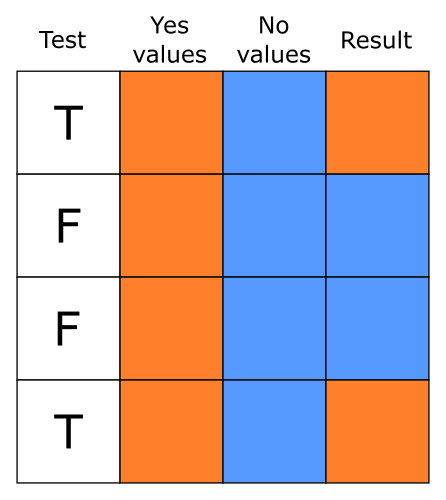
\includegraphics{Images/IfElse.png}

We'll also code neuroticism as either ``low'' or ``high'' based on
whether it's above the mean:

\begin{Shaded}
\begin{Highlighting}[]
\NormalTok{cow}\SpecialCharTok{$}\NormalTok{high\_neuroticism }\OtherTok{=} \FunctionTok{ifelse}\NormalTok{(}
\NormalTok{    cow}\SpecialCharTok{$}\NormalTok{neuroticism }\SpecialCharTok{\textgreater{}} \FunctionTok{mean}\NormalTok{(cow}\SpecialCharTok{$}\NormalTok{neuroticism),}
    \StringTok{"High"}\NormalTok{,}
    \StringTok{"Low"}
\NormalTok{)}
\NormalTok{cow}\SpecialCharTok{$}\NormalTok{high\_neuroticism }\OtherTok{=} \FunctionTok{factor}\NormalTok{(}
\NormalTok{    cow}\SpecialCharTok{$}\NormalTok{high\_neuroticism,}
    \AttributeTok{levels =} \FunctionTok{c}\NormalTok{(}\StringTok{"Low"}\NormalTok{, }\StringTok{"High"}\NormalTok{)}
\NormalTok{)}
\end{Highlighting}
\end{Shaded}

Since the example dataset we're using doesn't have
quite enough variables, let's also create a new one,
a score on a depression scale similar to PHQ-9:

\begin{Shaded}
\begin{Highlighting}[]
\CommentTok{\# Advanced code: run this but don\textquotesingle{}t worry too much about what}
\CommentTok{\#   it\textquotesingle{}s doing}
\FunctionTok{set.seed}\NormalTok{(}\DecValTok{1}\NormalTok{)}
\NormalTok{cow}\SpecialCharTok{$}\NormalTok{depression }\OtherTok{=} \FunctionTok{round}\NormalTok{(}
  \DecValTok{19} \SpecialCharTok{+} 
  \FloatTok{0.5} \SpecialCharTok{*}\NormalTok{ cow}\SpecialCharTok{$}\NormalTok{neuroticism }\SpecialCharTok{+}
  \SpecialCharTok{{-}}\FloatTok{0.8} \SpecialCharTok{*}\NormalTok{ cow}\SpecialCharTok{$}\NormalTok{extraversion }\SpecialCharTok{+}
  \FloatTok{0.5} \SpecialCharTok{*}\NormalTok{ (cow}\SpecialCharTok{$}\NormalTok{sex }\SpecialCharTok{==} \StringTok{"female"}\NormalTok{) }\SpecialCharTok{+}
  \FunctionTok{rnorm}\NormalTok{(}\FunctionTok{nrow}\NormalTok{(cow), }\AttributeTok{sd =} \DecValTok{3}\NormalTok{)}
\NormalTok{)}
\end{Highlighting}
\end{Shaded}

We'll recode this depression score into categories using
\texttt{cut()}, which allows us to divide up scores into
more than two categories:

\begin{Shaded}
\begin{Highlighting}[]
\NormalTok{cow}\SpecialCharTok{$}\NormalTok{depression\_diagnosis }\OtherTok{=} \FunctionTok{cut}\NormalTok{(}
\NormalTok{    cow}\SpecialCharTok{$}\NormalTok{depression,}
    \AttributeTok{breaks =} \FunctionTok{c}\NormalTok{(}\DecValTok{0}\NormalTok{, }\DecValTok{20}\NormalTok{, }\DecValTok{25}\NormalTok{, }\DecValTok{33}\NormalTok{),}
    \AttributeTok{labels =} \FunctionTok{c}\NormalTok{(}\StringTok{"None"}\NormalTok{, }\StringTok{"Mild"}\NormalTok{, }\StringTok{"Severe"}\NormalTok{),}
    \AttributeTok{include.lowest =} \ConstantTok{TRUE}
\NormalTok{)}
\end{Highlighting}
\end{Shaded}

\hypertarget{descriptive-statistics}{%
\section{Descriptive Statistics}\label{descriptive-statistics}}

Before doing any actual analysis it's always good to use
descriptive statistics to look at the data and get a sense
of what each variable looks like.

\hypertarget{quick-data-summary}{%
\subsection{Quick data summary}\label{quick-data-summary}}

You can get a good overview of the entire dataset using
\texttt{summary()}:

\begin{Shaded}
\begin{Highlighting}[]
\FunctionTok{summary}\NormalTok{(cow)}
\end{Highlighting}
\end{Shaded}

\begin{verbatim}
##   neuroticism     extraversion       sex      volunteer high_extraversion
##  Min.   : 0.00   Min.   : 2.00   female:780   no :824   Low :691         
##  1st Qu.: 8.00   1st Qu.:10.00   male  :641   yes:597   High:730         
##  Median :11.00   Median :13.00                                           
##  Mean   :11.47   Mean   :12.37                                           
##  3rd Qu.:15.00   3rd Qu.:15.00                                           
##  Max.   :24.00   Max.   :23.00                                           
##   personality_type high_neuroticism   depression    depression_diagnosis
##  Introvert:663     Low :722         Min.   : 0.00   None  :1195         
##  Extravert:758     High:699         1st Qu.:12.00   Mild  : 196         
##                                     Median :15.00   Severe:  30         
##                                     Mean   :15.07                       
##                                     3rd Qu.:18.00                       
##                                     Max.   :33.00
\end{verbatim}

\hypertarget{frequency-tables}{%
\subsection{Frequency tables}\label{frequency-tables}}

You can count frequencies of categorical variables with
\texttt{table()}:

\begin{Shaded}
\begin{Highlighting}[]
\FunctionTok{table}\NormalTok{(cow}\SpecialCharTok{$}\NormalTok{sex)}
\end{Highlighting}
\end{Shaded}

\begin{verbatim}
## 
## female   male 
##    780    641
\end{verbatim}

\begin{Shaded}
\begin{Highlighting}[]
\FunctionTok{table}\NormalTok{(cow}\SpecialCharTok{$}\NormalTok{sex, cow}\SpecialCharTok{$}\NormalTok{volunteer)}
\end{Highlighting}
\end{Shaded}

\begin{verbatim}
##         
##           no yes
##   female 431 349
##   male   393 248
\end{verbatim}

\hypertarget{histograms-distributions-of-continuous-variables}{%
\subsection{Histograms: distributions of continuous variables}\label{histograms-distributions-of-continuous-variables}}

Histograms are good for checking the range of scores
for a continuous variable to see if there are any
issues like skew, outlying scores etc.. Use \texttt{hist()}
to plot the histogram for a variable:

\begin{Shaded}
\begin{Highlighting}[]
\FunctionTok{hist}\NormalTok{(cow}\SpecialCharTok{$}\NormalTok{neuroticism)}
\end{Highlighting}
\end{Shaded}

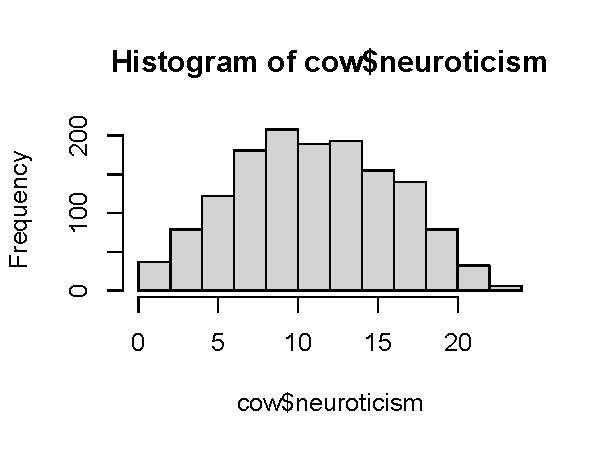
\includegraphics{Rad_files/figure-latex/hist_example-1.pdf}

\hypertarget{scatterplots-relationship-between-two-continuous-variables}{%
\subsection{Scatterplots: relationship between two continuous variables}\label{scatterplots-relationship-between-two-continuous-variables}}

Scatterplots are useful for getting a sense of whether or
not there's a relationship between two continuous variables.
The basic \texttt{plot()} function in R is quite flexible, so to
produce a scatter plot we just give it the two variables
and use \texttt{type\ =\ \textquotesingle{}p\textquotesingle{}} to indicate we want to plot points.

\begin{Shaded}
\begin{Highlighting}[]
\FunctionTok{plot}\NormalTok{(cow}\SpecialCharTok{$}\NormalTok{neuroticism, cow}\SpecialCharTok{$}\NormalTok{depression, }\AttributeTok{type=}\StringTok{\textquotesingle{}p\textquotesingle{}}\NormalTok{)}
\end{Highlighting}
\end{Shaded}

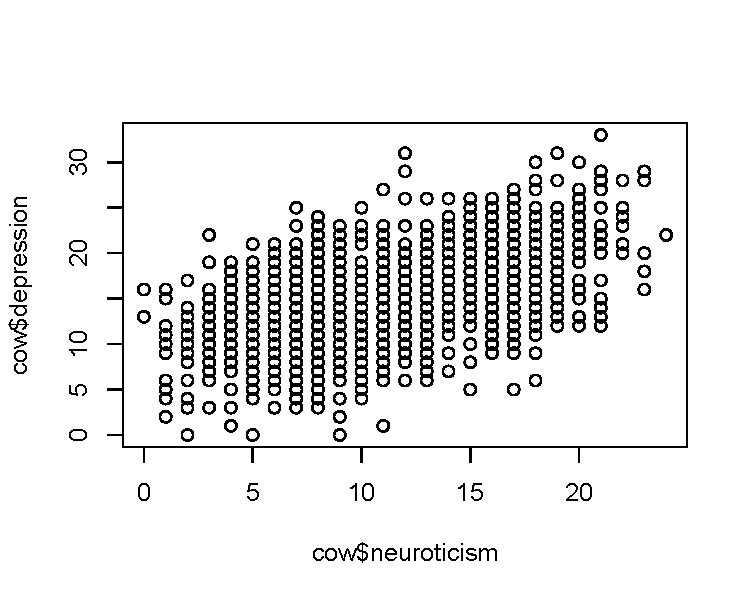
\includegraphics{Rad_files/figure-latex/scatter_example-1.pdf}

This plot doesn't look great - we'll cover ways to produce
better plots later. But you can see there's a positive
correlation between neuroticism and depression.\footnote{Keen readers will notice that the positive correlation is
  there because we put it there when generating the fake depression
  variable.}
To check the correlation we can use \texttt{cor()}:

\begin{Shaded}
\begin{Highlighting}[]
\FunctionTok{cor}\NormalTok{(cow}\SpecialCharTok{$}\NormalTok{neuroticism, cow}\SpecialCharTok{$}\NormalTok{depression)}
\end{Highlighting}
\end{Shaded}

\begin{verbatim}
## [1] 0.5341178
\end{verbatim}

\hypertarget{analysis}{%
\section{Analysis}\label{analysis}}

\hypertarget{t-test}{%
\subsection{T-test}\label{t-test}}

We can conduct a simple \emph{t} test of the differences in depression
scores between males and females using the \texttt{t.test()} function.
We can get the vector of scores for males and females by subsetting
and passing them to the function:

\begin{Shaded}
\begin{Highlighting}[]
\NormalTok{dep\_sex\_test }\OtherTok{=} \FunctionTok{t.test}\NormalTok{(cow}\SpecialCharTok{$}\NormalTok{depression[cow}\SpecialCharTok{$}\NormalTok{sex }\SpecialCharTok{==} \StringTok{"male"}\NormalTok{],}
\NormalTok{                      cow}\SpecialCharTok{$}\NormalTok{depression[cow}\SpecialCharTok{$}\NormalTok{sex }\SpecialCharTok{==} \StringTok{"female"}\NormalTok{])}
\NormalTok{dep\_sex\_test}
\end{Highlighting}
\end{Shaded}

\begin{verbatim}
## 
##  Welch Two Sample t-test
## 
## data:  cow$depression[cow$sex == "male"] and cow$depression[cow$sex == "female"]
## t = -4.275, df = 1356.4, p-value = 2.045e-05
## alternative hypothesis: true difference in means is not equal to 0
## 95 percent confidence interval:
##  -1.735880 -0.643867
## sample estimates:
## mean of x mean of y 
##  14.41654  15.60641
\end{verbatim}

Since we've saved the model object (basically a \texttt{list}) to a variable, we can
access the values we're most interested in if we need to use them again:

\begin{Shaded}
\begin{Highlighting}[]
\NormalTok{dep\_sex\_test}\SpecialCharTok{$}\NormalTok{p.value}
\end{Highlighting}
\end{Shaded}

\begin{verbatim}
## [1] 2.044769e-05
\end{verbatim}

To discover what values are available, you can look at the \textbf{Value}
section of the \texttt{?t.test} help page, or just type \texttt{dep\_sex\_test\$} and
let RStudio bring up the list of suggestions.

\hypertarget{formulas-a-simple-mini-language-for-expressing-models}{%
\subsection{Formulas: a simple mini-language for expressing models}\label{formulas-a-simple-mini-language-for-expressing-models}}

If we look at \texttt{?t.test}, we can see that there are actually
two different options for running a test: either pass two separate
vectors of scores representing the groups we want to compare,
or use a \textbf{formula}.

Formulas in R allow you to spell out models using a compact syntax,
allowing you to focus on the overall structure of your model. Formulas
in R contain \texttt{\textasciitilde{}} (a ``tilde''), with the outcome on the left of the \texttt{\textasciitilde{}} and
the predictors in the model on the right. For our t-test we have
\texttt{depression} as the outcome and \texttt{sex} as the grouping variable (our only
``predictor''). Running a \emph{t} test with a formula looks like:

\begin{Shaded}
\begin{Highlighting}[]
\FunctionTok{t.test}\NormalTok{(depression }\SpecialCharTok{\textasciitilde{}}\NormalTok{ sex, }\AttributeTok{data =}\NormalTok{ cow)}
\end{Highlighting}
\end{Shaded}

\begin{verbatim}
## 
##  Welch Two Sample t-test
## 
## data:  depression by sex
## t = 4.275, df = 1356.4, p-value = 2.045e-05
## alternative hypothesis: true difference in means between group female and group male is not equal to 0
## 95 percent confidence interval:
##  0.643867 1.735880
## sample estimates:
## mean in group female   mean in group male 
##             15.60641             14.41654
\end{verbatim}

When we're using a formula, we can usually use a \texttt{data\ =} argument
to say where all the variables in the model come from. R will automatically
look them up in the dataframe, without us having to access them manually.

\hypertarget{regression}{%
\subsection{Regression}\label{regression}}

We can also run a simple linear regression, prediction \texttt{depression}
(our outcome) using \texttt{neuroticism}, \texttt{extraversion} and \texttt{sex}. In R,
linear regression can be done using \texttt{lm()} (short for \textbf{l}inear
\textbf{m}odel). Our model looks like:

\begin{Shaded}
\begin{Highlighting}[]
\NormalTok{dep\_reg }\OtherTok{=} \FunctionTok{lm}\NormalTok{(depression }\SpecialCharTok{\textasciitilde{}}\NormalTok{ neuroticism }\SpecialCharTok{+}\NormalTok{ extraversion }\SpecialCharTok{+}\NormalTok{ sex,}
             \AttributeTok{data =}\NormalTok{ cow)}
\FunctionTok{summary}\NormalTok{(dep\_reg)}
\end{Highlighting}
\end{Shaded}

\begin{verbatim}
## 
## Call:
## lm(formula = depression ~ neuroticism + extraversion + sex, data = cow)
## 
## Residuals:
##     Min      1Q  Median      3Q     Max 
## -9.7374 -2.0909 -0.0555  2.1794 11.8903 
## 
## Coefficients:
##              Estimate Std. Error t value Pr(>|t|)    
## (Intercept)  19.72960    0.36979   53.35   <2e-16 ***
## neuroticism   0.49740    0.01707   29.13   <2e-16 ***
## extraversion -0.82358    0.02113  -38.98   <2e-16 ***
## sexmale      -0.38793    0.16718   -2.32   0.0205 *  
## ---
## Signif. codes:  0 '***' 0.001 '**' 0.01 '*' 0.05 '.' 0.1 ' ' 1
## 
## Residual standard error: 3.082 on 1417 degrees of freedom
## Multiple R-squared:  0.6553, Adjusted R-squared:  0.6545 
## F-statistic: 897.8 on 3 and 1417 DF,  p-value: < 2.2e-16
\end{verbatim}

\hypertarget{why-was-that-so-easy}{%
\subsubsection{Why was that so easy?}\label{why-was-that-so-easy}}

The regression model above was simple to fit because:

\begin{itemize}
\tightlist
\item
  We had all our data in a nice clean dataframe (in \textbf{long} format)
\item
  All our continuous variables were coded as numeric
\item
  All our categorical variables (\texttt{sex}) were coded as factors
\end{itemize}

Most of the setup for running models in R happens beforehand. Factors
will be treated as discrete variables, and numeric variables as
continuous variables, so make sure all your variables are the
right type before you try to fit a model.

If you don't have variables coded the right way, go back up
to the ``recoding'' section of your script and fix them there.

\hypertarget{formula-syntax}{%
\subsubsection{Formula syntax}\label{formula-syntax}}

The syntax you use in formulas is special, and it doesn't
necessarily mean the same thing as it would in regular R. For example
\texttt{+} doesn't mean ``add these values together'', it just means ``also
include this predictor''. The most important symbols in formula syntax
are:

\begin{itemize}
\tightlist
\item
  \texttt{+}: used to separate each individual predictor
\item
  \texttt{time:group}: \texttt{:} creates an interaction term between two variables,
  and only that interaction term.
\item
  \texttt{time*group}: \texttt{*} creates an interaction term between two variables,
  and also includes the individual main effects (\texttt{time} and \texttt{group} in
  this example). Usually more useful than \texttt{:} because interactions
  generally don't make sense without the main effects.
\item
  \texttt{1}: when you use \texttt{1} as a predictor on its own, it means ``include
  an intercept in the model''. This is the default so you don't
  have to include it. Intercepts make sense in most models.
\item
  \texttt{0}: signals that you don't want to fit an intercept. Not recommended
  most of the time.
\end{itemize}

\hypertarget{working-with-a-fitted-model}{%
\subsubsection{Working with a fitted model}\label{working-with-a-fitted-model}}

Once we've saved a fitted model to a variable, we can use it,
check it and save it in lots of different ways. The most
useful way is to call \texttt{summary(model)} like we did above,
which produces a summary table for the coefficients along
with a few useful statistics like \(R^2\).

There are also hundreds of different functions that people
have written to work with models and provide useful output,
both built in to R and available in packages. When possible,
look for a function that's already been written - there's no need
to reinvent the wheel. But if you want something that's not covered,
all the data you need is available, and you can use it to produce
exactly what you need.

\texttt{plot(model)}
(a built in command)
produces a few standard diagnostic plots that do things
like check the normality of your residuals and whether
particular outliers are affecting the fit:

\begin{Shaded}
\begin{Highlighting}[]
\CommentTok{\# This temporarily switches R\textquotesingle{}s plotting to a 2x2 layout}
\FunctionTok{par}\NormalTok{(}\AttributeTok{mfrow =} \FunctionTok{c}\NormalTok{(}\DecValTok{2}\NormalTok{, }\DecValTok{2}\NormalTok{))}
\FunctionTok{plot}\NormalTok{(dep\_reg)}
\end{Highlighting}
\end{Shaded}

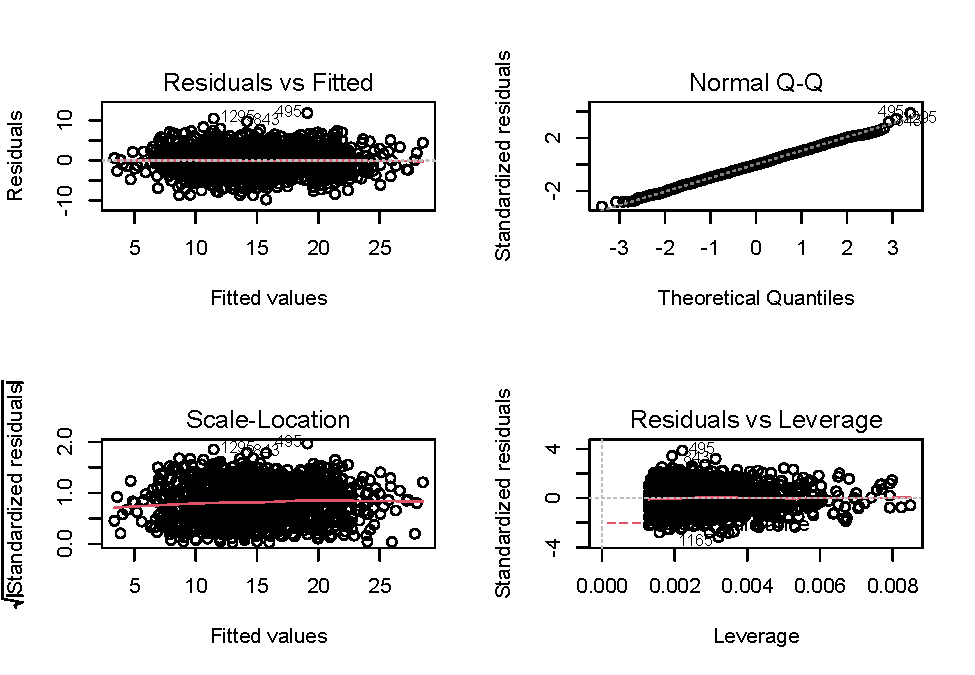
\includegraphics{Rad_files/figure-latex/plot_lm_example-1.pdf}

\begin{Shaded}
\begin{Highlighting}[]
\CommentTok{\# Switch plots back to normal}
\FunctionTok{par}\NormalTok{(}\AttributeTok{mfrow =} \FunctionTok{c}\NormalTok{(}\DecValTok{1}\NormalTok{, }\DecValTok{1}\NormalTok{))}
\end{Highlighting}
\end{Shaded}

\begin{note}
If you wanted to create the first plot from scratch, you could plot
\texttt{fitted(dep\_reg)} against \texttt{resid(dep\_reg)}.
\end{note}

\texttt{plot\_model} from the \texttt{sjPlot} package can give
us a nice visualisation of the effects in our model, automatically
choosing the right kind of plot for the predictor depending on
whether it's continuous or categorical:

\begin{Shaded}
\begin{Highlighting}[]
\FunctionTok{plot\_model}\NormalTok{(dep\_reg, }
           \CommentTok{\# We want to see the effect of each predictor,}
           \CommentTok{\#   but lots of other plot types are available}
           \AttributeTok{type =} \StringTok{"eff"}\NormalTok{,}
           \AttributeTok{terms =} \StringTok{"neuroticism"}\NormalTok{)}
\end{Highlighting}
\end{Shaded}

\begin{verbatim}
## Package `effects` is not available, but needed for `ggeffect()`. Either install package `effects`, or use `ggpredict()`. Calling `ggpredict()` now.FALSE
\end{verbatim}

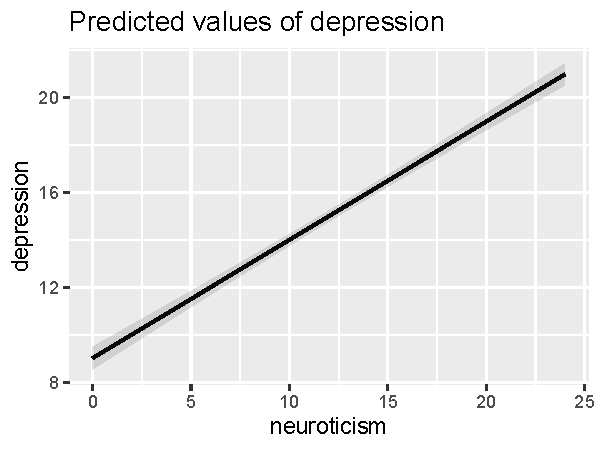
\includegraphics{Rad_files/figure-latex/plot_model_example-1.pdf}

\begin{Shaded}
\begin{Highlighting}[]
\FunctionTok{plot\_model}\NormalTok{(dep\_reg, }
           \AttributeTok{type =} \StringTok{"eff"}\NormalTok{,}
           \AttributeTok{terms =} \StringTok{"sex"}\NormalTok{)}
\end{Highlighting}
\end{Shaded}

\begin{verbatim}
## Package `effects` is not available, but needed for `ggeffect()`. Either install package `effects`, or use `ggpredict()`. Calling `ggpredict()` now.FALSE
\end{verbatim}

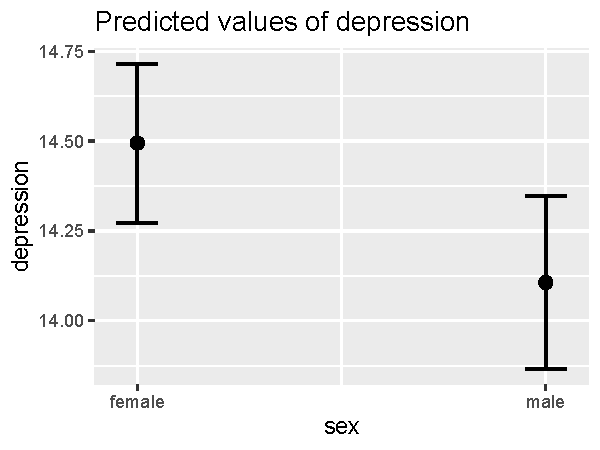
\includegraphics{Rad_files/figure-latex/plot_model_example-2.pdf}

You're also not stuck with the default presentation
of results from \texttt{summary()}, as there are lots of ways
to turn your model into a nice-looking table for publication.
\texttt{tab\_model()}, also from the \texttt{sjPlot} package, produces
good tables for regression models:

\begin{Shaded}
\begin{Highlighting}[]
\FunctionTok{tab\_model}\NormalTok{(dep\_reg)}
\end{Highlighting}
\end{Shaded}

\begin{figure}
\centering
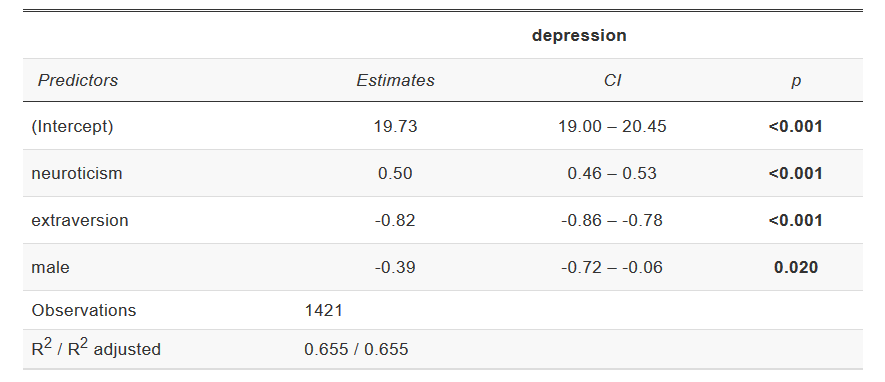
\includegraphics{Images/tab_model.png}
\caption{Example tab\_model output}
\end{figure}

\hypertarget{pointless-flashy-nonsense}{%
\section{Pointless flashy nonsense}\label{pointless-flashy-nonsense}}

Impress your friends and supervisors!

\textbf{NOTE:} Don't try to run this code (for now), it requires some
libraries that are tricky to install.

\begin{Shaded}
\begin{Highlighting}[]
\FunctionTok{library}\NormalTok{(rgl)}
\FunctionTok{library}\NormalTok{(rayshader)}

\NormalTok{hex\_gg }\OtherTok{=} \FunctionTok{ggplot}\NormalTok{(cow, }\FunctionTok{aes}\NormalTok{(}\AttributeTok{x =}\NormalTok{  neuroticism, }\AttributeTok{y =}\NormalTok{ extraversion)) }\SpecialCharTok{+}
    \FunctionTok{stat\_bin\_hex}\NormalTok{(}\FunctionTok{aes}\NormalTok{(}\AttributeTok{fill =} \FunctionTok{stat}\NormalTok{(density), }\AttributeTok{colour =} \FunctionTok{stat}\NormalTok{(density)), }
                 \AttributeTok{bins =} \DecValTok{10}\NormalTok{,}
                 \AttributeTok{size =} \DecValTok{1}\NormalTok{) }\SpecialCharTok{+}
    \FunctionTok{scale\_fill\_viridis\_c}\NormalTok{(}\AttributeTok{option =} \StringTok{"B"}\NormalTok{) }\SpecialCharTok{+}
    \FunctionTok{scale\_color\_viridis\_c}\NormalTok{(}\AttributeTok{option =} \StringTok{"B"}\NormalTok{, }\AttributeTok{guide =} \StringTok{"none"}\NormalTok{) }\SpecialCharTok{+}
    \FunctionTok{labs}\NormalTok{(}\AttributeTok{x =} \StringTok{"Neuroticism"}\NormalTok{, }\AttributeTok{y =} \StringTok{"Extraversion"}\NormalTok{, }\AttributeTok{fill =} \StringTok{""}\NormalTok{,}
         \AttributeTok{colour =} \StringTok{""}\NormalTok{) }\SpecialCharTok{+}
    \FunctionTok{theme\_minimal}\NormalTok{()}
\NormalTok{hex\_gg}

\FunctionTok{plot\_gg}\NormalTok{(hex\_gg, }\AttributeTok{multicore =} \ConstantTok{TRUE}\NormalTok{, }\AttributeTok{windowsize =} \FunctionTok{c}\NormalTok{(}\DecValTok{800}\NormalTok{, }\DecValTok{800}\NormalTok{))}
\FunctionTok{render\_movie}\NormalTok{(}\StringTok{"silly.mp4"}\NormalTok{, }\AttributeTok{phi =} \DecValTok{40}\NormalTok{, }\AttributeTok{theta =} \DecValTok{30}\NormalTok{)}
\end{Highlighting}
\end{Shaded}

\hypertarget{tidyverse}{%
\chapter{Easier analysis with the tidyverse}\label{tidyverse}}

Now that you know the basics of R, it's time to learn that there
are much better ways to do everything you just learnt!

\hypertarget{introduction-to-the-tidyverse}{%
\section{Introduction to the tidyverse}\label{introduction-to-the-tidyverse}}

The \href{https://www.tidyverse.org/}{tidyverse} is a bundle of packages that
make using R easier because they're all designed to work together. Most
``tidy'' functions work well together because they:

\begin{itemize}
\tightlist
\item
  Take a dataframe as their input
\item
  Return as dataframe as their output
\end{itemize}

You might not use every package from the \texttt{tidyverse} in an analysis,
but you can still load them all at the start of most analyses, and
know you'll have a standard set of tools available. To load
them all, just use:

\begin{Shaded}
\begin{Highlighting}[]
\FunctionTok{library}\NormalTok{(tidyverse)}
\end{Highlighting}
\end{Shaded}

For this session, we'll use the \texttt{cowles} data again, so let's
load it up:

\begin{Shaded}
\begin{Highlighting}[]
\NormalTok{cow }\OtherTok{=}\NormalTok{ carData}\SpecialCharTok{::}\NormalTok{Cowles}
\end{Highlighting}
\end{Shaded}

\hypertarget{dplyr-turning-complex-analyses-into-simple-steps}{%
\section{\texorpdfstring{\texttt{dplyr}: Turning complex analyses into simple steps}{dplyr: Turning complex analyses into simple steps}}\label{dplyr-turning-complex-analyses-into-simple-steps}}

\begin{figure}
\centering
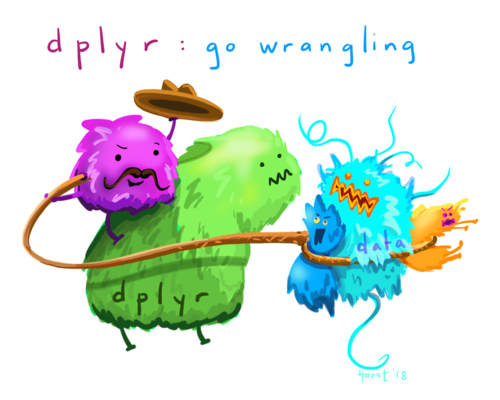
\includegraphics{Images/allisonhorst/dplyr_wrangling.png}
\caption{Artwork by @allison\_horst}
\end{figure}

As your analyses get more complicated, your code can get
more complicated as well. To get to the answers you want,
you might have to:

\begin{itemize}
\tightlist
\item
  Drop certain rows from your dataset because they're invalid
  or not relevant.
\item
  Calculate stats for each treatment group separately.
\item
  Use summary variables like the school mean to calculate
  a standardized score.
\end{itemize}

and more importantly, you might have to combine multiple
different operations like these for each calculation you're
doing.

The \texttt{dplyr} package in the tidyverse makes this easier
by providing a small number of simple \textbf{verbs} that can be combined
easily to perform complex tasks. Each one takes your current
data, changes it, and returns it. The most common verbs you'll
use are:

\begin{itemize}
\tightlist
\item
  \texttt{filter()}: choose rows to keep based on a logical test,
  dropping the rest.
\item
  \texttt{arrange()}: sort the data.
\item
  \texttt{select()}: choose columns to keep.
\item
  \texttt{mutate()}: add new columns.
\item
  \texttt{summarize()}: create columns that summarise the data down
  to a single row.
\item
  \texttt{count()}: Count the number of rows in the data.
\item
  \texttt{left\_join()} (and \texttt{right\_join()}, \texttt{inner\_join()} etc.): Merge datasets
  based on a common identifier.
\end{itemize}

And, possibly most importantly:

\begin{itemize}
\tightlist
\item
  \texttt{group\_by()}: Split the data into groups, so that any
  subsequent steps happen separately for each group.
\end{itemize}

We'll go over examples of all of these below.

\hypertarget{bending-the-rules-non-standard-evaluation}{%
\subsection{Bending the rules: Non-standard evaluation}\label{bending-the-rules-non-standard-evaluation}}

\texttt{dplyr} and other \texttt{tidyverse} packages bend the rules of R syntax,
allowing you to just type column names like \texttt{group} and \texttt{time} rather than
having to spell out the name of the dataframe each time (like \texttt{survey1\$group},
\texttt{survey1\$time}). \textbf{Within \texttt{tidyverse} function calls} you can just type the
column name, e.g.~

\begin{Shaded}
\begin{Highlighting}[]
\NormalTok{cow }\SpecialCharTok{\%\textgreater{}\%}
    \CommentTok{\# Within the brackets, no $ needed}
    \FunctionTok{count}\NormalTok{(sex, volunteer)}
\end{Highlighting}
\end{Shaded}

\begin{verbatim}
##      sex volunteer   n
## 1 female        no 431
## 2 female       yes 349
## 3   male        no 393
## 4   male       yes 248
\end{verbatim}

\hypertarget{pipes}{%
\subsection{\texorpdfstring{Pipes: \texttt{\%\textgreater{}\%}}{Pipes: \%\textgreater\%}}\label{pipes}}

\texttt{dplyr} and the \texttt{tidyverse} make heavy use of \textbf{pipes} to
make it easier to carry out multiple processing steps in a row.
A pipe looks like:

\begin{verbatim}
%>%
\end{verbatim}

If you have a calculation that takes multiple steps, it gets
confusing if you run them all in one go. Here we'll calculate
the mean of extraversion for the males in the data:

\begin{Shaded}
\begin{Highlighting}[]
\FunctionTok{summarise}\NormalTok{(}\FunctionTok{filter}\NormalTok{(cow, sex }\SpecialCharTok{==} \StringTok{"male"}\NormalTok{), }\AttributeTok{male\_mean =} \FunctionTok{mean}\NormalTok{(extraversion))}
\end{Highlighting}
\end{Shaded}

\begin{verbatim}
##   male_mean
## 1  12.31357
\end{verbatim}

The first step here is actually \texttt{filter}ing the data, but
we have to write these function calls \emph{inside out}. R understands
it fine but most human beings struggle to understand the logic
of what's happening, especially if there's more than 2 of
these \emph{nested} steps happening.

You can do the steps one by one instead, but it's clunky, and you
might have to create multiple intermediate variables:

\begin{Shaded}
\begin{Highlighting}[]
\NormalTok{males }\OtherTok{=} \FunctionTok{filter}\NormalTok{(cow, sex }\SpecialCharTok{==} \StringTok{"male"}\NormalTok{)}
\FunctionTok{summarise}\NormalTok{(males, }\AttributeTok{male\_mean =} \FunctionTok{mean}\NormalTok{(extraversion))}
\end{Highlighting}
\end{Shaded}

Using pipes, you can do each step, and then send it \textbf{through
the pipe} to the next step. To get the mean extraversion
for males using pipes, we can do:

\begin{Shaded}
\begin{Highlighting}[]
\NormalTok{cow }\SpecialCharTok{\%\textgreater{}\%}
    \FunctionTok{filter}\NormalTok{(sex }\SpecialCharTok{==} \StringTok{"male"}\NormalTok{) }\SpecialCharTok{\%\textgreater{}\%}
    \FunctionTok{summarise}\NormalTok{(}\AttributeTok{male\_mean =} \FunctionTok{mean}\NormalTok{(extraversion))}
\end{Highlighting}
\end{Shaded}

\begin{verbatim}
##   male_mean
## 1  12.31357
\end{verbatim}

See how we're not actually specifying a dataframe for the
\texttt{filter()} and \texttt{summarise()} functions? That's because
the \texttt{\%\textgreater{}\%} pipe \textbf{automatically sends the data as
the first argument to the next function}.

\hypertarget{common-tasks-with-dplyr}{%
\subsection{\texorpdfstring{Common tasks with \texttt{dplyr}}{Common tasks with dplyr}}\label{common-tasks-with-dplyr}}

\hypertarget{selecting-columns-with-select}{%
\subsubsection*{\texorpdfstring{Selecting columns with \texttt{select}}{Selecting columns with select}}\label{selecting-columns-with-select}}
\addcontentsline{toc}{subsubsection}{Selecting columns with \texttt{select}}

You can select particular columns from a dataframe using \texttt{select()}. Using
\texttt{-} in front of a column name excludes that column:

\begin{Shaded}
\begin{Highlighting}[]
\CommentTok{\# These both give the same result: inclusion vs. exclusion}
\NormalTok{cow }\SpecialCharTok{\%\textgreater{}\%}
    \FunctionTok{select}\NormalTok{(neuroticism, extraversion) }\SpecialCharTok{\%\textgreater{}\%}
    \FunctionTok{head}\NormalTok{(}\DecValTok{2}\NormalTok{)}
\end{Highlighting}
\end{Shaded}

\begin{verbatim}
##   neuroticism extraversion
## 1          16           13
## 2           8           14
\end{verbatim}

\begin{Shaded}
\begin{Highlighting}[]
\NormalTok{cow }\SpecialCharTok{\%\textgreater{}\%}
    \FunctionTok{select}\NormalTok{(}\SpecialCharTok{{-}}\NormalTok{sex, }\SpecialCharTok{{-}}\NormalTok{volunteer) }\SpecialCharTok{\%\textgreater{}\%} 
    \FunctionTok{head}\NormalTok{(}\DecValTok{2}\NormalTok{)}
\end{Highlighting}
\end{Shaded}

\begin{verbatim}
##   neuroticism extraversion
## 1          16           13
## 2           8           14
\end{verbatim}

Instead of column names, you can also use a range of helper functions
like \texttt{starts\_with()} and \texttt{num\_range()} to select multiple columns
that match a particular pattern.

\hypertarget{creatingchanging-columns-with-mutate}{%
\subsubsection*{\texorpdfstring{Creating/changing columns with \texttt{mutate}}{Creating/changing columns with mutate}}\label{creatingchanging-columns-with-mutate}}
\addcontentsline{toc}{subsubsection}{Creating/changing columns with \texttt{mutate}}

We can use \texttt{mutate} on a dataframe to add or change one or more columns:

\begin{Shaded}
\begin{Highlighting}[]
\NormalTok{cow }\SpecialCharTok{\%\textgreater{}\%}
    \CommentTok{\# high\_extraversion and high\_neuroticism are the names}
    \CommentTok{\#   of new columns that will be created}
    \FunctionTok{mutate}\NormalTok{(}\AttributeTok{high\_extraversion =}\NormalTok{ extraversion }\SpecialCharTok{\textgreater{}=} \DecValTok{15}\NormalTok{,}
           \AttributeTok{high\_neuroticism =}\NormalTok{ neuroticism }\SpecialCharTok{\textgreater{}=} \DecValTok{15}\NormalTok{) }\SpecialCharTok{\%\textgreater{}\%}
    \FunctionTok{head}\NormalTok{()}
\end{Highlighting}
\end{Shaded}

\begin{verbatim}
##   neuroticism extraversion    sex volunteer high_extraversion high_neuroticism
## 1          16           13 female        no             FALSE             TRUE
## 2           8           14   male        no             FALSE            FALSE
## 3           5           16   male        no              TRUE            FALSE
## 4           8           20 female        no              TRUE            FALSE
## 5           9           19   male        no              TRUE            FALSE
## 6           6           15   male        no              TRUE            FALSE
\end{verbatim}

If we want these changes to be saved, we would need to \textbf{save the
result back to the original variable}. By default, \texttt{mutate()} will
just return an altered copy of the original data, but won't change
the original:

\begin{Shaded}
\begin{Highlighting}[]
\CommentTok{\# If we want to actually save the changes}
\NormalTok{cow }\OtherTok{=}\NormalTok{ cow }\SpecialCharTok{\%\textgreater{}\%}
    \FunctionTok{mutate}\NormalTok{(}\AttributeTok{high\_extraversion =}\NormalTok{ extraversion }\SpecialCharTok{\textgreater{}=} \DecValTok{15}\NormalTok{,}
           \AttributeTok{high\_neuroticism =}\NormalTok{ neuroticism }\SpecialCharTok{\textgreater{}=} \DecValTok{15}\NormalTok{)}
\end{Highlighting}
\end{Shaded}

On its own, the main advantage \texttt{mutate} offers is being able to spell
out your calculations without including the name of the dataframe. However,
it can be very useful in combination with other verbs.

\hypertarget{summarizing-the-data-with-summarize}{%
\subsubsection*{\texorpdfstring{Summarizing the data with \texttt{summarize}}{Summarizing the data with summarize}}\label{summarizing-the-data-with-summarize}}
\addcontentsline{toc}{subsubsection}{Summarizing the data with \texttt{summarize}}

\texttt{summarize} is similar to \texttt{mutate}: it adds or changes columns. However,
\texttt{summarize} also \textbf{collapses the data down to a single row}, so the
values you calculate need to be single values like means or counts.

\begin{Shaded}
\begin{Highlighting}[]
\NormalTok{cow }\SpecialCharTok{\%\textgreater{}\%}
    \FunctionTok{summarize}\NormalTok{(}
        \AttributeTok{extraversion =} \FunctionTok{mean}\NormalTok{(extraversion),}
        \AttributeTok{volunteers =} \FunctionTok{sum}\NormalTok{(volunteer }\SpecialCharTok{==} \StringTok{"yes"}\NormalTok{)}
\NormalTok{    )}
\end{Highlighting}
\end{Shaded}

\begin{verbatim}
##   extraversion volunteers
## 1     12.37298        597
\end{verbatim}

\texttt{summarize} is useful in combination with \texttt{group\_by}, where it
collapses the data down to \textbf{one row per group}.

\hypertarget{selecting-rows-with-filter}{%
\subsubsection*{\texorpdfstring{Selecting rows with \texttt{filter}}{Selecting rows with filter}}\label{selecting-rows-with-filter}}
\addcontentsline{toc}{subsubsection}{Selecting rows with \texttt{filter}}

Choosing rows with a logical test with \texttt{filter()} works just like
subsetting your data with a logical vector, it's just easier
to do it as part of a sequence of steps:

\begin{Shaded}
\begin{Highlighting}[]
\NormalTok{cow }\SpecialCharTok{\%\textgreater{}\%}
  \FunctionTok{filter}\NormalTok{((sex }\SpecialCharTok{==} \StringTok{"male"}\NormalTok{) }\SpecialCharTok{\&}\NormalTok{ (volunteer }\SpecialCharTok{==} \StringTok{"yes"}\NormalTok{)) }\SpecialCharTok{\%\textgreater{}\%}
  \FunctionTok{head}\NormalTok{()}
\end{Highlighting}
\end{Shaded}

\begin{verbatim}
##     neuroticism extraversion  sex volunteer
## 220          17           19 male       yes
## 439           7           15 male       yes
## 440          17           12 male       yes
## 442           6           13 male       yes
## 445           8            9 male       yes
## 446           5           16 male       yes
\end{verbatim}

\hypertarget{sorting-with-arrange}{%
\subsubsection*{\texorpdfstring{Sorting with \texttt{arrange}}{Sorting with arrange}}\label{sorting-with-arrange}}
\addcontentsline{toc}{subsubsection}{Sorting with \texttt{arrange}}

With \texttt{arrange}, you can sort by one or more columns. Use \texttt{desc(column)}
(short for \textbf{descending}) to sort that column in the opposite direction:

\begin{Shaded}
\begin{Highlighting}[]
\NormalTok{cow }\SpecialCharTok{\%\textgreater{}\%}
  \FunctionTok{arrange}\NormalTok{(sex, volunteer, }\FunctionTok{desc}\NormalTok{(extraversion)) }\SpecialCharTok{\%\textgreater{}\%}
  \FunctionTok{head}\NormalTok{()}
\end{Highlighting}
\end{Shaded}

\begin{verbatim}
##      neuroticism extraversion    sex volunteer
## 1109          15           23 female        no
## 67            15           21 female        no
## 277            9           21 female        no
## 875           10           21 female        no
## 4              8           20 female        no
## 40             5           20 female        no
\end{verbatim}

\hypertarget{group_by-for-calculations-within-groups}{%
\subsubsection*{\texorpdfstring{\texttt{group\_by} for calculations within groups}{group\_by for calculations within groups}}\label{group_by-for-calculations-within-groups}}
\addcontentsline{toc}{subsubsection}{\texttt{group\_by} for calculations within groups}

\texttt{group\_by()} is very useful for calculating different stats in
subgroups of your data. This covers a \emph{lot} of the more complex
operations you might need to do with your data, so it unlocks
a lot of possibilities.

You can do things like:

\begin{itemize}
\tightlist
\item
  Mean-centering scores separately for males and females:
\end{itemize}

\begin{Shaded}
\begin{Highlighting}[]
\NormalTok{cow }\SpecialCharTok{\%\textgreater{}\%}
    \FunctionTok{group\_by}\NormalTok{(sex) }\SpecialCharTok{\%\textgreater{}\%}
    \FunctionTok{mutate}\NormalTok{(}
        \AttributeTok{extraversion\_centered =}\NormalTok{ extraversion }\SpecialCharTok{{-}} \FunctionTok{mean}\NormalTok{(extraversion)}
\NormalTok{    )}
\end{Highlighting}
\end{Shaded}

\begin{verbatim}
## # A tibble: 1,421 x 5
## # Groups:   sex [2]
##    neuroticism extraversion sex    volunteer extraversion_centered
##          <int>        <int> <fct>  <fct>                     <dbl>
##  1          16           13 female no                        0.578
##  2           8           14 male   no                        1.69 
##  3           5           16 male   no                        3.69 
##  4           8           20 female no                        7.58 
##  5           9           19 male   no                        6.69 
##  6           6           15 male   no                        2.69 
##  7           8           10 female no                       -2.42 
##  8          12           11 male   no                       -1.31 
##  9          15           16 male   no                        3.69 
## 10          18            7 male   no                       -5.31 
## # ... with 1,411 more rows
\end{verbatim}

\begin{itemize}
\tightlist
\item
  Calculating means and SDs for subgroups:
\end{itemize}

\begin{Shaded}
\begin{Highlighting}[]
\NormalTok{cow }\SpecialCharTok{\%\textgreater{}\%}
    \FunctionTok{group\_by}\NormalTok{(sex, volunteer) }\SpecialCharTok{\%\textgreater{}\%}
    \FunctionTok{summarise}\NormalTok{(}\AttributeTok{mean =} \FunctionTok{mean}\NormalTok{(neuroticism),}
              \AttributeTok{sd =} \FunctionTok{sd}\NormalTok{(neuroticism))}
\end{Highlighting}
\end{Shaded}

\begin{verbatim}
## `summarise()` has grouped output by 'sex'. You can override using the `.groups`
## argument.
\end{verbatim}

\begin{verbatim}
## # A tibble: 4 x 4
## # Groups:   sex [2]
##   sex    volunteer  mean    sd
##   <fct>  <fct>     <dbl> <dbl>
## 1 female no         12.2  4.75
## 2 female yes        12.3  4.79
## 3 male   no         10.5  4.75
## 4 male   yes        10.4  5.11
\end{verbatim}

\hypertarget{frequency-tables-with-count}{%
\subsubsection*{\texorpdfstring{Frequency tables with \texttt{count}}{Frequency tables with count}}\label{frequency-tables-with-count}}
\addcontentsline{toc}{subsubsection}{Frequency tables with \texttt{count}}

\texttt{count()} gives you a straightforward way to create a frequency table. There's
no built-in way to calculate percentages, but you can easily add them
using \texttt{mutate()}:

\begin{Shaded}
\begin{Highlighting}[]
\NormalTok{cow }\SpecialCharTok{\%\textgreater{}\%}
    \FunctionTok{count}\NormalTok{(sex) }\SpecialCharTok{\%\textgreater{}\%}
    \CommentTok{\# count creates a column called \textquotesingle{}n\textquotesingle{}}
    \FunctionTok{mutate}\NormalTok{(}\AttributeTok{percent =}\NormalTok{ n }\SpecialCharTok{/} \FunctionTok{sum}\NormalTok{(n) }\SpecialCharTok{*} \DecValTok{100}\NormalTok{)}
\end{Highlighting}
\end{Shaded}

\begin{verbatim}
##      sex   n  percent
## 1 female 780 54.89092
## 2   male 641 45.10908
\end{verbatim}

If you have multiple levels of grouping, you need to think about
how you want to calculate percentages. To get the percentage
who volunteered within each sex:

\begin{Shaded}
\begin{Highlighting}[]
\NormalTok{cow }\SpecialCharTok{\%\textgreater{}\%}
    \FunctionTok{count}\NormalTok{(sex, volunteer) }\SpecialCharTok{\%\textgreater{}\%}
    \FunctionTok{group\_by}\NormalTok{(sex) }\SpecialCharTok{\%\textgreater{}\%}
    \FunctionTok{mutate}\NormalTok{(}\AttributeTok{percent =}\NormalTok{ n }\SpecialCharTok{/} \FunctionTok{sum}\NormalTok{(n) }\SpecialCharTok{*} \DecValTok{100}\NormalTok{)}
\end{Highlighting}
\end{Shaded}

\begin{verbatim}
## # A tibble: 4 x 4
## # Groups:   sex [2]
##   sex    volunteer     n percent
##   <fct>  <fct>     <int>   <dbl>
## 1 female no          431    55.3
## 2 female yes         349    44.7
## 3 male   no          393    61.3
## 4 male   yes         248    38.7
\end{verbatim}

\hypertarget{merging-data-with-left_join}{%
\subsubsection{\texorpdfstring{Merging data with \texttt{left\_join()}}{Merging data with left\_join()}}\label{merging-data-with-left_join}}

To combine two dataframes, you can use functions like \texttt{left\_join()}
and \texttt{inner\_join()}. In my experience, \texttt{left\_join()} is what you
want most of the time. To merge data successfully, all you
need is a column that's present in both datasets that they can
be matched on, usually a participant ID or something similar.

Joins can also be useful when you have to calculate a complex
summary. You can create a separate table with the summary info,
and merge it back into the main dataset. As a simple example,
let's summarize extraversion by both sex and volunteering
status and merge it back into the main dataset:

\begin{Shaded}
\begin{Highlighting}[]
\NormalTok{extraversion\_info }\OtherTok{=}\NormalTok{ cow }\SpecialCharTok{\%\textgreater{}\%}
    \FunctionTok{group\_by}\NormalTok{(sex, volunteer) }\SpecialCharTok{\%\textgreater{}\%}
    \FunctionTok{summarize}\NormalTok{(}\AttributeTok{mean\_extraversion =} \FunctionTok{mean}\NormalTok{(extraversion))}
\end{Highlighting}
\end{Shaded}

\begin{verbatim}
## `summarise()` has grouped output by 'sex'. You can override using the `.groups`
## argument.
\end{verbatim}

\begin{Shaded}
\begin{Highlighting}[]
\NormalTok{extraversion\_info}
\end{Highlighting}
\end{Shaded}

\begin{verbatim}
## # A tibble: 4 x 3
## # Groups:   sex [2]
##   sex    volunteer mean_extraversion
##   <fct>  <fct>                 <dbl>
## 1 female no                     12.0
## 2 female yes                    12.9
## 3 male   no                     11.9
## 4 male   yes                    12.9
\end{verbatim}

\begin{Shaded}
\begin{Highlighting}[]
\NormalTok{cow }\SpecialCharTok{\%\textgreater{}\%}
    \FunctionTok{left\_join}\NormalTok{(extraversion\_info, }\AttributeTok{by =} \FunctionTok{c}\NormalTok{(}\StringTok{"sex"}\NormalTok{, }\StringTok{"volunteer"}\NormalTok{)) }\SpecialCharTok{\%\textgreater{}\%}
    \FunctionTok{head}\NormalTok{()}
\end{Highlighting}
\end{Shaded}

\begin{verbatim}
##   neuroticism extraversion    sex volunteer mean_extraversion
## 1          16           13 female        no          12.00696
## 2           8           14   male        no          11.91349
## 3           5           16   male        no          11.91349
## 4           8           20 female        no          12.00696
## 5           9           19   male        no          11.91349
## 6           6           15   male        no          11.91349
\end{verbatim}

\hypertarget{better-plots-with-ggplot2}{%
\chapter{\texorpdfstring{Better plots with \texttt{ggplot2}}{Better plots with ggplot2}}\label{better-plots-with-ggplot2}}

R's plotting tools are very good, and in particular, there's
a great library called \texttt{ggplot2} that allows you to put together
a huge variety out of plots using a simple system and some
common pieces.

\texttt{ggplot2} is loaded whenever you use \texttt{library(tidyverse)},
but you can also load it individually:

\begin{Shaded}
\begin{Highlighting}[]
\FunctionTok{library}\NormalTok{(ggplot2)}

\NormalTok{cow }\OtherTok{=}\NormalTok{ carData}\SpecialCharTok{::}\NormalTok{Cowles}
\CommentTok{\# Recreating the depression variable from before}
\FunctionTok{set.seed}\NormalTok{(}\DecValTok{1}\NormalTok{)}
\NormalTok{cow}\SpecialCharTok{$}\NormalTok{depression }\OtherTok{=} \FunctionTok{round}\NormalTok{(}
  \DecValTok{19} \SpecialCharTok{+} 
  \FloatTok{0.5} \SpecialCharTok{*}\NormalTok{ cow}\SpecialCharTok{$}\NormalTok{neuroticism }\SpecialCharTok{+}
  \SpecialCharTok{{-}}\FloatTok{0.8} \SpecialCharTok{*}\NormalTok{ cow}\SpecialCharTok{$}\NormalTok{extraversion }\SpecialCharTok{+}
  \FloatTok{0.5} \SpecialCharTok{*}\NormalTok{ (cow}\SpecialCharTok{$}\NormalTok{sex }\SpecialCharTok{==} \StringTok{"female"}\NormalTok{) }\SpecialCharTok{+}
  \FunctionTok{rnorm}\NormalTok{(}\FunctionTok{nrow}\NormalTok{(cow), }\AttributeTok{sd =} \DecValTok{3}\NormalTok{)}
\NormalTok{)}
\end{Highlighting}
\end{Shaded}

\hypertarget{using-ggplot2-properly}{%
\section{\texorpdfstring{Using \texttt{ggplot2} properly}{Using ggplot2 properly}}\label{using-ggplot2-properly}}

\texttt{ggplot2} will always work best if:

\begin{itemize}
\tightlist
\item
  Everything you want to show in the plot is
  in a single dataframe.
\item
  Each aspect of the plot is represented by a single
  column.
\item
  Each column has the right data type, depending
  on whether it's categorical or continuous
  (\texttt{factor} or \texttt{numeric}).
\item
  All the data is labelled: categorical variables
  should already have the labels that you want to show in the plot.
\end{itemize}

You can make plots work if you don't have have those
things, but they will be much clunkier to put together.
Take the time to put the data into the right shape
before you try to produce a plot.

\hypertarget{mapping-aesthetics}{%
\section{Mapping aesthetics}\label{mapping-aesthetics}}

The most important concept in \texttt{ggplot2} is \textbf{mapping}
each variable in the data to an \textbf{aesthetic} feature
of the plot. A wide variety of plots can be put together
using a small number of common aesthetics. The aesthetic
mapping for a plot is set up using the \texttt{aes()} function.

Think about a scatterplot - one variable is mapped
to the position along the x-axis, and another
is mapped to the position along the y-axis. So
a basic scatterplot in ggplot is:

\begin{Shaded}
\begin{Highlighting}[]
\FunctionTok{ggplot}\NormalTok{(cow, }\FunctionTok{aes}\NormalTok{(}\AttributeTok{x =}\NormalTok{ neuroticism, }\AttributeTok{y =}\NormalTok{ depression)) }\SpecialCharTok{+}
    \FunctionTok{geom\_point}\NormalTok{()}
\end{Highlighting}
\end{Shaded}

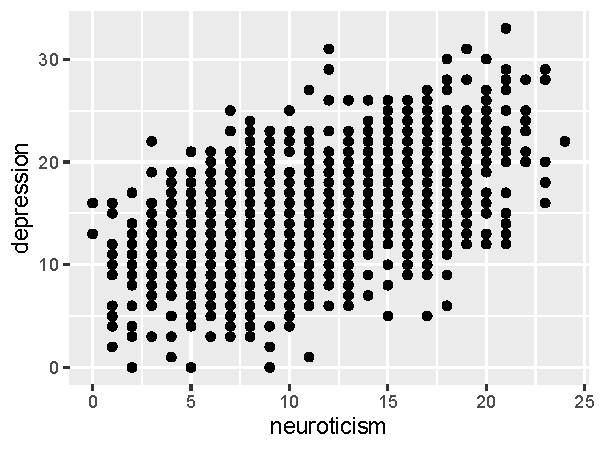
\includegraphics{Rad_files/figure-latex/basic_ggplot_scatterplot-1.pdf}

You could also map another variable to the colour of the points:

\begin{Shaded}
\begin{Highlighting}[]
\FunctionTok{ggplot}\NormalTok{(cow, }
       \FunctionTok{aes}\NormalTok{(}\AttributeTok{x =}\NormalTok{ neuroticism, }\AttributeTok{y =}\NormalTok{ depression, }\AttributeTok{colour =}\NormalTok{ sex)) }\SpecialCharTok{+}
    \FunctionTok{geom\_point}\NormalTok{()}
\end{Highlighting}
\end{Shaded}

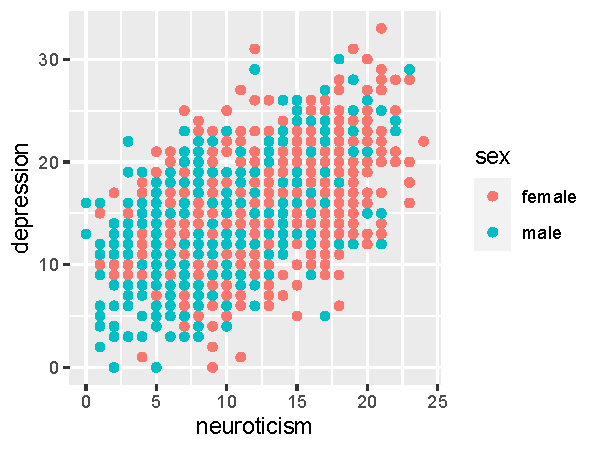
\includegraphics{Rad_files/figure-latex/ggplot_scatter_colours-1.pdf}

Sometimes you want to change the look of \emph{everything} in the plot,
without it being specific to individual data points. In that
case, you don't put it in the \texttt{aes()} mapping, you \textbf{set it as an
argument for the geom you want to change}. Everything
that \textbf{varies based on data} should still go in \texttt{aes()}. For
example, when scatterplots have lots of points it helps
to make them transparent so you can see how many points
are overlapping:

\begin{Shaded}
\begin{Highlighting}[]
\FunctionTok{ggplot}\NormalTok{(cow, }
       \FunctionTok{aes}\NormalTok{(}\AttributeTok{x =}\NormalTok{ neuroticism, }\AttributeTok{y =}\NormalTok{ depression, }\AttributeTok{colour =}\NormalTok{ sex)) }\SpecialCharTok{+}
    \FunctionTok{geom\_point}\NormalTok{(}\AttributeTok{alpha =} \FloatTok{0.4}\NormalTok{)}
\end{Highlighting}
\end{Shaded}

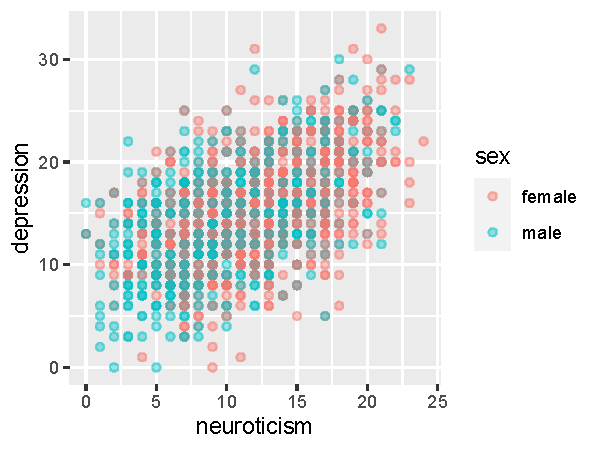
\includegraphics{Rad_files/figure-latex/ggplot_scatter_alpha-1.pdf}

\hypertarget{geoms-representing-the-data-with-different-components}{%
\section{geoms: representing the data with different components}\label{geoms-representing-the-data-with-different-components}}

\texttt{ggplot2} doesn't have functions for specific kinds of plots
like a ``boxplot'' or ``bar chart''. It does have all the components
you need to put these together though.

A boxplot will usually have:

\begin{itemize}
\tightlist
\item
  A categorical variable mapped to \texttt{x}
\item
  A continuous variable mapped to \texttt{y}
\item
  Possibly extra variables mapped to the ``fill colour'' of
  the boxes.
\end{itemize}

\begin{Shaded}
\begin{Highlighting}[]
\FunctionTok{ggplot}\NormalTok{(cow, }\FunctionTok{aes}\NormalTok{(}\AttributeTok{x =}\NormalTok{ sex, }\AttributeTok{y =}\NormalTok{ depression, }\AttributeTok{fill =}\NormalTok{ volunteer)) }\SpecialCharTok{+}
    \FunctionTok{geom\_boxplot}\NormalTok{()}
\end{Highlighting}
\end{Shaded}

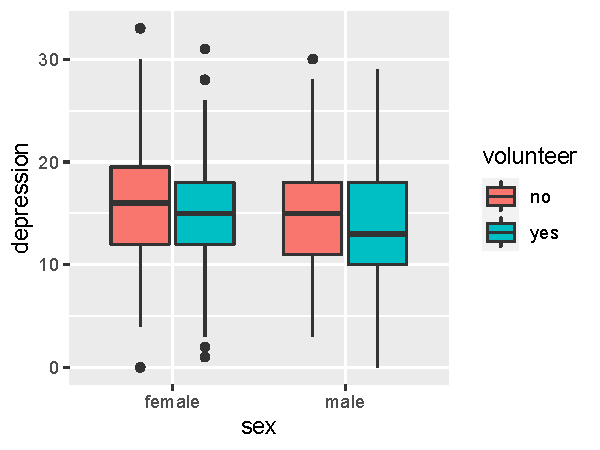
\includegraphics{Rad_files/figure-latex/ggplot_boxplot_example-1.pdf}

A bar chart will usually have:

\begin{itemize}
\tightlist
\item
  A discrete variable mapped to \texttt{x}
\item
  Another variable mapped to \texttt{fill} that defines
  the subgroups.
\item
  No variable mapped to \texttt{y}: \texttt{y} in a bar chart is
  normally just the count (number of rows) in
  each subgroup.
\item
  The bars for the subgroups either ``stacked'' on top
  of each other or side by side (ggplot2 calls this
  ``dodging'')
\end{itemize}

\begin{Shaded}
\begin{Highlighting}[]
\FunctionTok{ggplot}\NormalTok{(cow, }\FunctionTok{aes}\NormalTok{(}\AttributeTok{x =}\NormalTok{ sex, }\AttributeTok{fill =}\NormalTok{ volunteer)) }\SpecialCharTok{+}
    \FunctionTok{geom\_bar}\NormalTok{(}\AttributeTok{position =} \StringTok{"dodge"}\NormalTok{)}
\end{Highlighting}
\end{Shaded}

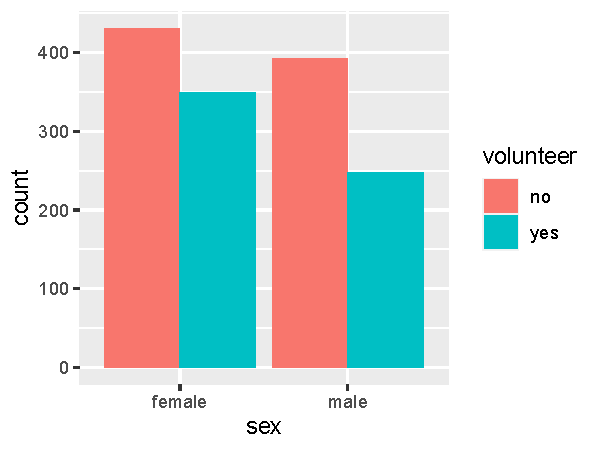
\includegraphics{Rad_files/figure-latex/ggplot_bar_example-1.pdf}

We've done some very standard plot types here
to help illustrate how each plot can be broken down
into its aesthetic mappings, but the real power
of ggplot is that you aren't tied to the standard
kinds of plots - you can mix and match their
components to produce a unique plot that shows
exactly what you want.

\hypertarget{combining-geoms}{%
\section{Combining geoms}\label{combining-geoms}}

Here we'll produce a plot that shows:

\begin{itemize}
\tightlist
\item
  The individual data points (``jittered'' a bit so they
  don't all overlap)
\item
  Contours that show how dense the points are
\item
  A ``line of best fit'' that shows the overall relationship
  between two variables
\end{itemize}

When you plot multiple geoms, the order you put them
together defines which element will be on top - the
first geom is on the bottom.

\begin{Shaded}
\begin{Highlighting}[]
\FunctionTok{ggplot}\NormalTok{(cow, }\FunctionTok{aes}\NormalTok{(}\AttributeTok{x =}\NormalTok{ neuroticism, }\AttributeTok{y =}\NormalTok{ depression)) }\SpecialCharTok{+}
    \FunctionTok{stat\_density\_2d}\NormalTok{(}\FunctionTok{aes}\NormalTok{(}\AttributeTok{fill =} \FunctionTok{stat}\NormalTok{(level)),}
                    \AttributeTok{geom =} \StringTok{"polygon"}\NormalTok{,}
                    \AttributeTok{alpha =} \FloatTok{0.6}\NormalTok{) }\SpecialCharTok{+}
    \FunctionTok{geom\_jitter}\NormalTok{(}\AttributeTok{alpha =} \FloatTok{0.5}\NormalTok{) }\SpecialCharTok{+}
    \FunctionTok{geom\_smooth}\NormalTok{(}\AttributeTok{colour =} \StringTok{"red"}\NormalTok{) }\SpecialCharTok{+}
    \FunctionTok{scale\_fill\_viridis\_c}\NormalTok{() }\SpecialCharTok{+}
    \FunctionTok{theme\_bw}\NormalTok{()}
\end{Highlighting}
\end{Shaded}

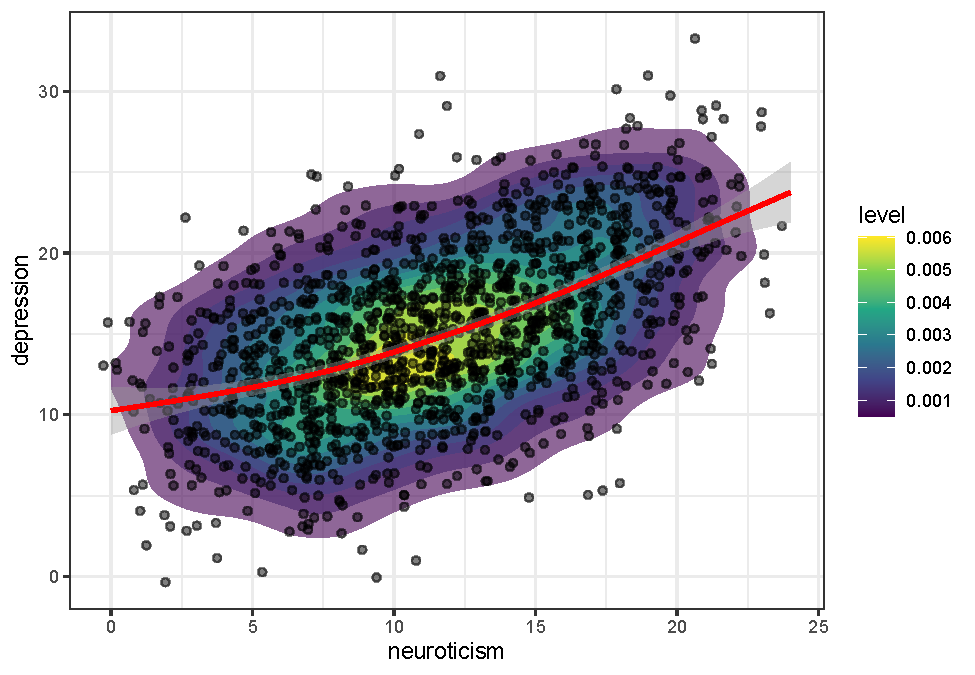
\includegraphics{Rad_files/figure-latex/ggplot_complex_example-1.pdf}

This plot is probably a little bit too ``busy'' to be really useful -
when you have so many options for what you can fit in a plot,
you have to make good choices about what's most important to
include.

\hypertarget{scales-and-themes-changing-the-look-of-your-plot}{%
\section{Scales and themes: changing the look of your plot}\label{scales-and-themes-changing-the-look-of-your-plot}}

Once you have a functioning \texttt{ggplot} plot put together,
you can start customising the look of it easily by using
different \textbf{scales} (which change how a variable maps
to a particular aesthetic feature of the plot) and
\textbf{themes} (which change more general elements
of the plot like the background colour).

\hypertarget{scales}{%
\subsection{Scales}\label{scales}}

Scales serve a few different purposes:

\begin{itemize}
\tightlist
\item
  Changing the order of values: e.g.~reversing the order on the x-axis
\item
  Transforming values, e.g.~log-transforming your y-axis
\item
  Choosing how your values will be represented - particularly their
  \textbf{colours}.
\end{itemize}

The scales in ggplot generally have two parts to their names, like
\texttt{scale\_x\_log10()} and \texttt{scale\_colour\_gradient()}. The two parts indicate:

\begin{itemize}
\tightlist
\item
  Which aesthetic of the plot the scale is for.
\item
  What kind of scale will be applied for that aesthetic
\end{itemize}

\hypertarget{scale-examples}{%
\subsubsection*{Scale examples}\label{scale-examples}}
\addcontentsline{toc}{subsubsection}{Scale examples}

If you just need to reverse the order of a continuous x or y-axis, use
\texttt{scale\_x\_reverse()} or \texttt{scale\_y\_reverse()}. Returning to our
scatter plot from above:

\begin{Shaded}
\begin{Highlighting}[]
\FunctionTok{ggplot}\NormalTok{(cow, }
       \FunctionTok{aes}\NormalTok{(}\AttributeTok{x =}\NormalTok{ neuroticism, }\AttributeTok{y =}\NormalTok{ depression, }\AttributeTok{colour =}\NormalTok{ sex)) }\SpecialCharTok{+}
    \FunctionTok{geom\_point}\NormalTok{(}\AttributeTok{alpha =} \FloatTok{0.4}\NormalTok{) }\SpecialCharTok{+}
    \FunctionTok{scale\_y\_reverse}\NormalTok{()}
\end{Highlighting}
\end{Shaded}

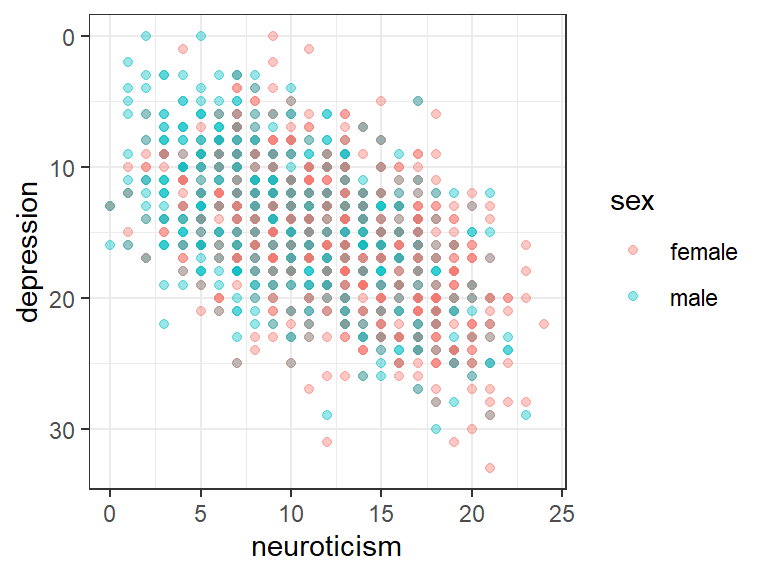
\includegraphics{Rad_files/figure-latex/ggplot_scatter_reversed-1.png}

Log-transforms can be useful for variables like income that are skewed
and have a few very large values. Use \texttt{scale\_x\_log10()} or \texttt{scale\_y\_log10()},
and note how the axis increases in multiples rather than a constant rate:

\begin{Shaded}
\begin{Highlighting}[]
\FunctionTok{ggplot}\NormalTok{(cow, }\FunctionTok{aes}\NormalTok{(}\AttributeTok{x =}\NormalTok{ sex, }\AttributeTok{fill =}\NormalTok{ volunteer)) }\SpecialCharTok{+}
    \FunctionTok{geom\_bar}\NormalTok{(}\AttributeTok{position =} \StringTok{"dodge"}\NormalTok{) }\SpecialCharTok{+}
    \FunctionTok{scale\_y\_log10}\NormalTok{()}
\end{Highlighting}
\end{Shaded}

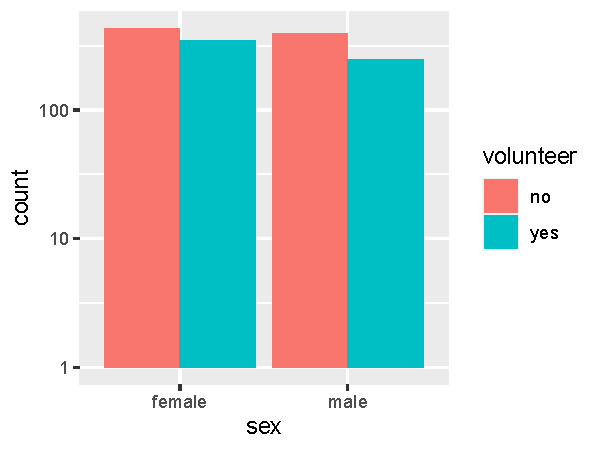
\includegraphics{Rad_files/figure-latex/ggplot_log_example-1.pdf}

Changing the colour scale you're using in your plot is useful both
because you can pick a more meaningful scale, and because it can
really improve the overall look and clarity of your plot. Picking
colours that look good is a valid reason!

To demonstrate some of these colour scales, we'll first create
a categorical variable that splits our depression scores up into
5 categories. We'll also create a table of the mean neuroticism
and extraversion scores in each category:

\begin{Shaded}
\begin{Highlighting}[]
\NormalTok{cow}\SpecialCharTok{$}\NormalTok{depression\_cat }\OtherTok{=} \FunctionTok{cut}\NormalTok{(}
\NormalTok{    cow}\SpecialCharTok{$}\NormalTok{depression, }\AttributeTok{breaks =} \DecValTok{5}\NormalTok{,}
    \AttributeTok{labels =} \FunctionTok{c}\NormalTok{(}\StringTok{"Very low"}\NormalTok{, }\StringTok{"Low"}\NormalTok{, }\StringTok{"Average"}\NormalTok{,}
               \StringTok{"High"}\NormalTok{, }\StringTok{"Very high"}\NormalTok{))}

\NormalTok{dep\_tab }\OtherTok{=}\NormalTok{ cow }\SpecialCharTok{\%\textgreater{}\%}
    \FunctionTok{group\_by}\NormalTok{(depression\_cat) }\SpecialCharTok{\%\textgreater{}\%}
    \FunctionTok{summarize}\NormalTok{(}\AttributeTok{introversion =} \FunctionTok{mean}\NormalTok{(neuroticism),}
              \AttributeTok{extraversion =} \FunctionTok{mean}\NormalTok{(extraversion)) }\SpecialCharTok{\%\textgreater{}\%}
    \FunctionTok{pivot\_longer}\NormalTok{(}\SpecialCharTok{{-}}\NormalTok{depression\_cat, }
                 \AttributeTok{names\_to =} \StringTok{"Outcome"}\NormalTok{,}
                 \AttributeTok{values\_to =} \StringTok{"Mean"}\NormalTok{)}
\end{Highlighting}
\end{Shaded}

Plotting with the default colours doesn't give great results:

\begin{Shaded}
\begin{Highlighting}[]
\NormalTok{dep\_cat\_plot }\OtherTok{=} \FunctionTok{ggplot}\NormalTok{(}
\NormalTok{    dep\_tab, }
    \FunctionTok{aes}\NormalTok{(}\AttributeTok{x =}\NormalTok{ Outcome, }\AttributeTok{y =}\NormalTok{ Mean, }\AttributeTok{fill =}\NormalTok{ depression\_cat)) }\SpecialCharTok{+}
    \FunctionTok{geom\_col}\NormalTok{(}\AttributeTok{position =} \StringTok{\textquotesingle{}dodge\textquotesingle{}}\NormalTok{, }\AttributeTok{colour =} \StringTok{\textquotesingle{}black\textquotesingle{}}\NormalTok{) }\SpecialCharTok{+}
    \CommentTok{\# \textbackslash{}n creates a newline, i.e. splits the label into multiple lines}
    \FunctionTok{labs}\NormalTok{(}\AttributeTok{fill =} \StringTok{"Depression}\SpecialCharTok{\textbackslash{}n}\StringTok{Category"}\NormalTok{) }\SpecialCharTok{+}
    \FunctionTok{theme\_bw}\NormalTok{()}

\NormalTok{dep\_cat\_plot}
\end{Highlighting}
\end{Shaded}

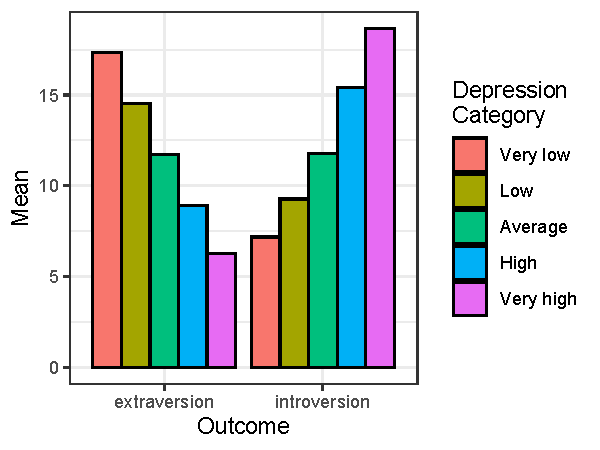
\includegraphics{Rad_files/figure-latex/dep_cat_default-1.pdf}

Since the categories are increasing, we could use a colour scale
that maps colours in an ordered way. The \texttt{viridis} colour scales
look great and have a few useful properties like converting to
greyscale well and being colour-blind friendly. Using an ordered
colour scale helps to convey some of the meaning of the different
depression categories:

\begin{Shaded}
\begin{Highlighting}[]
\NormalTok{dep\_cat\_plot }\SpecialCharTok{+} 
    \CommentTok{\# Tweaked slightly to avoid using a very bright yellow}
    \CommentTok{\#   at the top end of the scale}
    \FunctionTok{scale\_fill\_viridis\_d}\NormalTok{(}\AttributeTok{option =} \StringTok{"C"}\NormalTok{, }\AttributeTok{end =} \FloatTok{0.9}\NormalTok{)}
\end{Highlighting}
\end{Shaded}

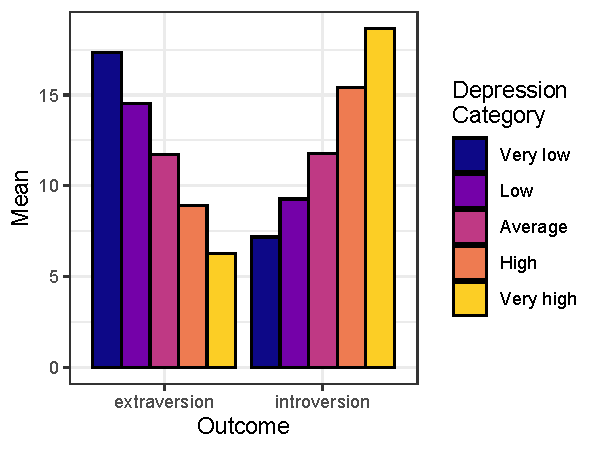
\includegraphics{Rad_files/figure-latex/dep_cat_viridis-1.pdf}

\begin{note}
The aesthetic that determines the colour of the bars is \texttt{fill},
not \texttt{colour}, so we use \texttt{scale\_fill} to change it. Check
whether your plot is using the \texttt{fill} or the \texttt{colour}
aesthetic to make sure you change the right one.
\end{note}

We could also use a \textbf{diverging} colour scale that emphasises
how far each category is from the average. ggplot includes
some great scales from \href{http://colorbrewer2.org/}{ColorBrewer} that
serve this purpose:

\begin{Shaded}
\begin{Highlighting}[]
\NormalTok{dep\_cat\_plot }\SpecialCharTok{+} 
    \FunctionTok{scale\_fill\_brewer}\NormalTok{(}\AttributeTok{type =} \StringTok{"div"}\NormalTok{)}
\end{Highlighting}
\end{Shaded}

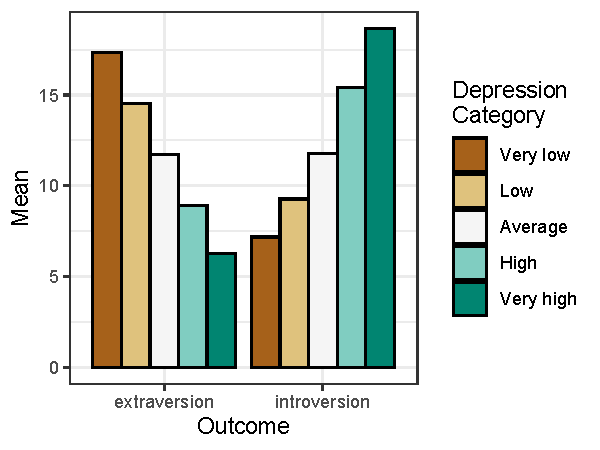
\includegraphics{Rad_files/figure-latex/dep_cat_diverging-1.pdf}

Feel free to experiment with different scales when producing
your own plots!

\hypertarget{themes}{%
\subsection{Themes}\label{themes}}

Scales affect how your actual data is displayed, but to control the
overall look of the plot (background colour, font etc.), we use
\textbf{themes}. To use a different theme, just add it to your plot:

\begin{Shaded}
\begin{Highlighting}[]
\NormalTok{dep\_cat\_plot }\SpecialCharTok{+}
    \FunctionTok{scale\_fill\_viridis\_d}\NormalTok{() }\SpecialCharTok{+}
    \FunctionTok{theme\_classic}\NormalTok{()}
\end{Highlighting}
\end{Shaded}

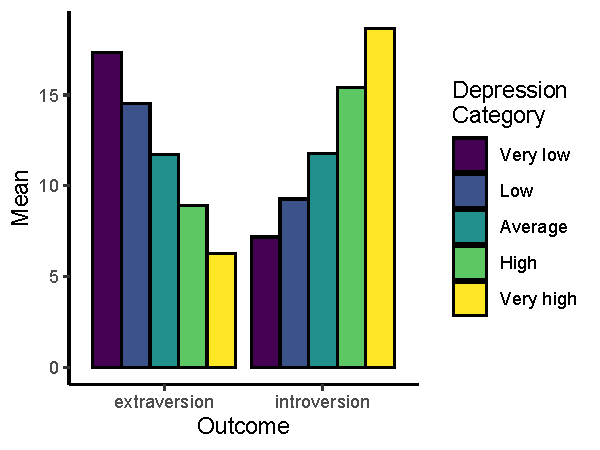
\includegraphics{Rad_files/figure-latex/ggplot_theming_example-1.pdf}

\begin{Shaded}
\begin{Highlighting}[]
\CommentTok{\# sjPlot should have been installed during an earlier}
\CommentTok{\#   session, otherwise install it now}
\NormalTok{dep\_cat\_plot }\SpecialCharTok{+}
    \FunctionTok{scale\_fill\_viridis\_d}\NormalTok{() }\SpecialCharTok{+}
\NormalTok{    sjPlot}\SpecialCharTok{::}\FunctionTok{theme\_538}\NormalTok{()}
\end{Highlighting}
\end{Shaded}

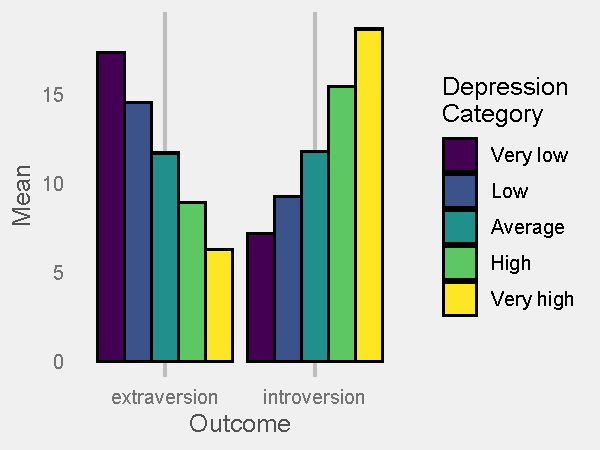
\includegraphics{Rad_files/figure-latex/ggplot_theming_example-2.pdf}

\hypertarget{tweaking-themes}{%
\subsubsection{Tweaking themes}\label{tweaking-themes}}

Every aspect of a plot's theme can be tweaked using \texttt{theme()}.
You can see the full list of properties that can be changed by looking
at \texttt{?theme}.
The full details are beyond the scope of this brief introduction,
but one useful tweak is turning off particular elements by setting
them to \texttt{element\_blank()}. We can disable the title on the x-axis:

\begin{Shaded}
\begin{Highlighting}[]
\NormalTok{dep\_cat\_plot }\SpecialCharTok{+}
    \FunctionTok{scale\_fill\_viridis\_d}\NormalTok{() }\SpecialCharTok{+}
    \FunctionTok{theme}\NormalTok{(}\AttributeTok{axis.title.x =} \FunctionTok{element\_blank}\NormalTok{())}
\end{Highlighting}
\end{Shaded}

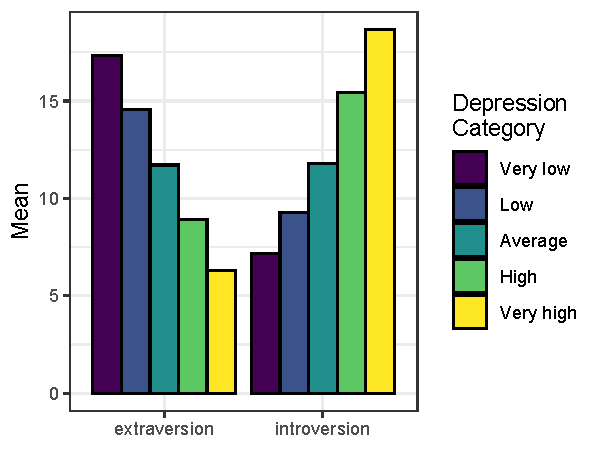
\includegraphics{Rad_files/figure-latex/theme_tweak_example-1.pdf}

\hypertarget{finding-extra-scales-and-themes}{%
\subsection{Finding extra scales and themes}\label{finding-extra-scales-and-themes}}

Packages like \texttt{ggthemes} provide extra scales and themes: install
them, load them and you can use the scales and themes just like
the built in ones by adding them to your plot. I particularly like
\texttt{ggthemes::theme\_fivethirtyeight()}
and \texttt{ggthemes::scale\_colour\_tableau()}, but there a wide variety
of useful and great-looking options out there.

\hypertarget{other-packages-use-ggplot2-too}{%
\section{\texorpdfstring{Other packages use \texttt{ggplot2} too}{Other packages use ggplot2 too}}\label{other-packages-use-ggplot2-too}}

\hypertarget{real-world-data-example}{%
\chapter{Real world data example}\label{real-world-data-example}}

In this example, we'll use some data derived from a real study to get
some experience dealing with messy raw data \footnote{All the data used here was simulated with
  \href{https://cran.r-project.org/web/packages/synthpop/index.html}{synthpop},
  so it doesn't contain data from any actual participants.}.

Before we start, we'll install some packages:

\begin{Shaded}
\begin{Highlighting}[]
\FunctionTok{install.packages}\NormalTok{(}\FunctionTok{c}\NormalTok{(}\StringTok{"readxl"}\NormalTok{, }\StringTok{"lme4"}\NormalTok{))}
\end{Highlighting}
\end{Shaded}

\hypertarget{data-overview}{%
\section{Data overview}\label{data-overview}}

This data contains the post-treatment observations from a
cluster-randomised trial comparing a novel treatment to control.
Schools were randomised to different groups, so every
participant in the same school received the same
intervention. It contains:

\begin{itemize}
\tightlist
\item
  SURPS scores, a scale assessing different personality traits
  associated with substance use.
\item
  The anxiety and depression subscales of the Brief Symptom Inventory
\item
  Questions about alcohol use
\end{itemize}

The scales haven't been scored, so our first step will be scoring
them, before we move onto describing and analysing the data.

\begin{note}
Checking what you've just done is very useful after any change you make
to the data. Throughout this example, I'll include notes on how you
could check the previous step. Try to code those checks yourself!
\end{note}

\hypertarget{surps-overview}{%
\subsection{SURPS overview}\label{surps-overview}}

The SURPS scale has four subscales:

\begin{itemize}
\tightlist
\item
  Negative thinking/hopelessness
\item
  Anxiety sensitivity
\item
  Impulsivity
\item
  Sensation seeking
\end{itemize}

Higher scores on each subscale represent higher levels
of the personality traits related to substance use, i.e.
greater risk.

\hypertarget{bsi-overview}{%
\subsection{BSI overview}\label{bsi-overview}}

The study includes two subscales from the Brief Symptom Inventory.
Higher scores on each represent higher levels of symptoms:

\begin{itemize}
\tightlist
\item
  Depression
\item
  Anxiety
\end{itemize}

\hypertarget{basic-setup}{%
\section{Basic setup}\label{basic-setup}}

\hypertarget{load-libraries}{%
\subsection{Load libraries}\label{load-libraries}}

As always, the first step is loading the libraries we'll use in this
analysis:

\begin{Shaded}
\begin{Highlighting}[]
\FunctionTok{library}\NormalTok{(tidyverse)}
\FunctionTok{library}\NormalTok{(psych)}
\FunctionTok{library}\NormalTok{(sjPlot)}
\FunctionTok{library}\NormalTok{(readxl)}
\FunctionTok{library}\NormalTok{(lme4)}

\CommentTok{\# We\textquotesingle{}ll also set a default theme for our}
\CommentTok{\#   ggplot plots}
\FunctionTok{theme\_set}\NormalTok{(}\FunctionTok{theme\_bw}\NormalTok{())}
\end{Highlighting}
\end{Shaded}

\hypertarget{load-the-data}{%
\subsection{Load the data}\label{load-the-data}}

The example data is available online - to download it you can use:

\begin{Shaded}
\begin{Highlighting}[]
\FunctionTok{download.file}\NormalTok{(}\StringTok{"https://gitlab.com/warsquid/rad/raw/master/data/CapSimulatedData.xlsx"}\NormalTok{,}
              \AttributeTok{destfile =} \StringTok{"CapSimulatedData.xlsx"}\NormalTok{,}
              \AttributeTok{mode =} \StringTok{"wb"}\NormalTok{)}
\end{Highlighting}
\end{Shaded}

(if that doesn't work, please manually download the file
\href{https://gitlab.com/warsquid/rad/raw/master/data/CapSimulatedData.xlsx}{here}
and copy it to your project directory)

Now we can load the data in:

\begin{Shaded}
\begin{Highlighting}[]
\NormalTok{real }\OtherTok{=}\NormalTok{ readxl}\SpecialCharTok{::}\FunctionTok{read\_excel}\NormalTok{(}\StringTok{"CapSimulatedData.xlsx"}\NormalTok{)}
\FunctionTok{head}\NormalTok{(real)}
\end{Highlighting}
\end{Shaded}

\begin{verbatim}
## # A tibble: 6 x 43
##   PersonId SchoolId Sex   Group Surps1 Surps2 Surps3 Surps4 Surps5 Surps6 Surps7
##      <dbl>    <dbl> <chr> <chr>  <dbl>  <dbl>  <dbl>  <dbl>  <dbl>  <dbl>  <dbl>
## 1        1        2 Male  Cont~      3      1      1      2      2      2      2
## 2        2        7 Fema~ Cont~     NA     NA     NA     NA     NA     NA     NA
## 3        3        2 Male  Trea~      2      1      3      2      0      3      2
## 4        4        1 Male  Cont~     NA     NA     NA     NA     NA     NA     NA
## 5        5        6 Male  Cont~      3      1      2      2      1      2      2
## 6        6       14 Male  Trea~      3      1      2      3      0      3      3
## # ... with 32 more variables: Surps8 <dbl>, Surps9 <dbl>, Surps10 <dbl>,
## #   Surps11 <dbl>, Surps12 <dbl>, Surps13 <dbl>, Surps14 <dbl>, Surps15 <dbl>,
## #   Surps16 <dbl>, Surps17 <dbl>, Surps18 <dbl>, Surps19 <dbl>, Surps20 <dbl>,
## #   Surps21 <dbl>, Surps22 <dbl>, Surps23 <dbl>, Bsi1 <dbl>, Bsi2 <dbl>,
## #   Bsi3 <dbl>, Bsi4 <dbl>, Bsi5 <dbl>, Bsi6 <dbl>, Bsi7 <dbl>, Bsi8 <dbl>,
## #   Bsi9 <dbl>, Bsi10 <dbl>, SipEver <dbl>, FullEver <dbl>, Sip6 <dbl>,
## #   Full6 <dbl>, Full6_freq <dbl>, PresentPost <dbl>
\end{verbatim}

A good first step is to use \texttt{str()} to inspect the data types:

\begin{Shaded}
\begin{Highlighting}[]
\FunctionTok{str}\NormalTok{(real)}
\end{Highlighting}
\end{Shaded}

And check some basic features of the data like the number of people
in each intervention group (and maybe school?).

\begin{Shaded}
\begin{Highlighting}[]
\FunctionTok{table}\NormalTok{(real}\SpecialCharTok{$}\NormalTok{Group)}
\end{Highlighting}
\end{Shaded}

\begin{verbatim}
## 
##   Control Treatment 
##      1001      1189
\end{verbatim}

\begin{Shaded}
\begin{Highlighting}[]
\FunctionTok{table}\NormalTok{(real}\SpecialCharTok{$}\NormalTok{SchoolId)}
\end{Highlighting}
\end{Shaded}

\begin{verbatim}
## 
##   1   2   3   4   5   6   7   8   9  10  11  12  13  14  15  16  17  18  19  20 
## 112 114 113  88 126  93 118 125 106  96 108 115 105  96 116 115 108 110 105 121
\end{verbatim}

\hypertarget{solve-major-issues}{%
\subsection{Solve major issues}\label{solve-major-issues}}

One major issue with this data is that not everyone completed the
post-treatment assessment, and they have missing data for all
the questions. In an in-depth analysis we might try to handle
this missing data in a more sophisticated way, but for now there's
not much we can do with it, so we'll drop it up front:

\begin{Shaded}
\begin{Highlighting}[]
\CommentTok{\# Same as:}
\CommentTok{\# real = real[real$PresentPost == 1, ]}
\NormalTok{real }\OtherTok{=} \FunctionTok{filter}\NormalTok{(real, PresentPost }\SpecialCharTok{==} \DecValTok{1}\NormalTok{)}
\end{Highlighting}
\end{Shaded}

This is a contrived example, but if you can do something
to simplify your data like this, it's best to do it up front,
before getting into the details of data cleaning and analysis.

\hypertarget{recoding-and-scoring}{%
\section{Recoding and scoring}\label{recoding-and-scoring}}

\hypertarget{scoring-surps-the-easy-way}{%
\subsection{Scoring SURPS the easy way}\label{scoring-surps-the-easy-way}}

Sometimes there are existing functions in R or in packages that people
have written that do exactly what we want with minimal effort.

The \texttt{psych::scoreItems()} function is designed for scoring psychometric
scales, and it has options to allow a few common tweaks to the scoring
process, so it will often score things exactly how you want them.

The most useful feature of \texttt{scoreItems()} is it allows you to specify the questions
that make up each subscale by providing a \textbf{list}: each element
of the list is a \textbf{character vector} specifying which questions
are in that subscale. You can put a \texttt{-} in front of a question
if that question should be \textbf{reverse scored}.

So a simple scale with two subscales might look like:

\begin{Shaded}
\begin{Highlighting}[]
\NormalTok{scoring\_key }\OtherTok{=} \FunctionTok{list}\NormalTok{(}
    \AttributeTok{Extraversion =} \FunctionTok{c}\NormalTok{(}\StringTok{"Q1"}\NormalTok{, }\StringTok{"{-}Q2"}\NormalTok{, }\StringTok{"Q3"}\NormalTok{),}
    \AttributeTok{Introversion =} \FunctionTok{c}\NormalTok{(}\StringTok{"{-}Q4"}\NormalTok{, }\StringTok{"{-}Q5"}\NormalTok{, }\StringTok{"Q6"}\NormalTok{)}
\NormalTok{)}
\end{Highlighting}
\end{Shaded}

The SURPS questionnaire has four subscales, and we can score them all at once
using:

\begin{Shaded}
\begin{Highlighting}[]
\NormalTok{surps\_keys }\OtherTok{=} \FunctionTok{list}\NormalTok{(}
    \AttributeTok{Nt =} \FunctionTok{c}\NormalTok{(}\StringTok{"{-}Surps1"}\NormalTok{, }\StringTok{"{-}Surps4"}\NormalTok{, }\StringTok{"{-}Surps7"}\NormalTok{, }\StringTok{"{-}Surps13"}\NormalTok{, }
           \StringTok{"Surps17"}\NormalTok{, }\StringTok{"{-}Surps20"}\NormalTok{, }\StringTok{"{-}Surps23"}\NormalTok{),}
    \AttributeTok{As =} \FunctionTok{c}\NormalTok{(}\StringTok{"Surps8"}\NormalTok{, }\StringTok{"Surps10"}\NormalTok{, }\StringTok{"Surps14"}\NormalTok{, }\StringTok{"Surps18"}\NormalTok{, }
           \StringTok{"Surps21"}\NormalTok{),}
    \AttributeTok{Imp =} \FunctionTok{c}\NormalTok{(}\StringTok{"Surps2"}\NormalTok{, }\StringTok{"Surps5"}\NormalTok{, }\StringTok{"Surps11"}\NormalTok{, }\StringTok{"Surps15"}\NormalTok{, }
            \StringTok{"Surps22"}\NormalTok{),}
    \AttributeTok{Ss =} \FunctionTok{c}\NormalTok{(}\StringTok{"Surps3"}\NormalTok{, }\StringTok{"Surps6"}\NormalTok{, }\StringTok{"Surps9"}\NormalTok{, }\StringTok{"Surps12"}\NormalTok{, }
               \StringTok{"Surps16"}\NormalTok{, }\StringTok{"Surps19"}\NormalTok{)}
\NormalTok{)}

\NormalTok{surps\_scored }\OtherTok{=}\NormalTok{ psych}\SpecialCharTok{::}\FunctionTok{scoreItems}\NormalTok{(}
    \AttributeTok{keys =}\NormalTok{ surps\_keys, }
    \AttributeTok{items =}\NormalTok{ real,}
    \AttributeTok{totals =} \ConstantTok{TRUE}\NormalTok{,}
    \AttributeTok{impute =} \StringTok{"median"}\NormalTok{)}
\end{Highlighting}
\end{Shaded}

We have the scores now, but we haven't added them to our main dataset yet.
We can look at the object that \texttt{scoreItems()} has given us:

\begin{Shaded}
\begin{Highlighting}[]
\NormalTok{surps\_scored}
\end{Highlighting}
\end{Shaded}

This is a lot of information, and right now we're only interested in the scores,
so we need to check how to access them.

Looking at the help page \texttt{?scoreItems} under the \textbf{Value} section tells us the
actual scores are stored at \texttt{surps\_scored\$scores}. We can add all 4 columns into
our dataset at once with:

\begin{Shaded}
\begin{Highlighting}[]
\NormalTok{real[, }\FunctionTok{c}\NormalTok{(}\StringTok{"NtTotal"}\NormalTok{, }\StringTok{"AsTotal"}\NormalTok{, }\StringTok{"ImpTotal"}\NormalTok{, }\StringTok{"SsTotal"}\NormalTok{)] }\OtherTok{=}\NormalTok{ surps\_scored}\SpecialCharTok{$}\NormalTok{scores}
\FunctionTok{head}\NormalTok{(real[, }\FunctionTok{c}\NormalTok{(}\StringTok{"NtTotal"}\NormalTok{, }\StringTok{"AsTotal"}\NormalTok{, }\StringTok{"ImpTotal"}\NormalTok{, }\StringTok{"SsTotal"}\NormalTok{)])}
\end{Highlighting}
\end{Shaded}

\begin{verbatim}
## # A tibble: 6 x 4
##   NtTotal AsTotal ImpTotal SsTotal
##     <dbl>   <dbl>    <dbl>   <dbl>
## 1       7       6        7       7
## 2       6      11        5      12
## 3       6       6        5      11
## 4       0       3        2      11
## 5       8       8        5      12
## 6       6       1        9      12
\end{verbatim}

\begin{note}
Sometimes you don't need all the extra info that
\texttt{psych::scoreItems()} provides. \texttt{psych::scoreFast()} will
do the same calculations but just return the final scores.
\end{note}

\hypertarget{scoring-surps-the-harder-way}{%
\subsection{Scoring SURPS the harder way}\label{scoring-surps-the-harder-way}}

Functions like \texttt{scoreItems()} won't always do exactly what we want.
When we scored the scales above, we let \texttt{scoreItems()} impute any missing
values using that item's median score. However, if we have our own missing
data procedure that doesn't match what \texttt{scoreItems()} does, we might have
to do some of the work ourselves.

One scoring procedure I've used in the past is:

\begin{itemize}
\tightlist
\item
  Calculate the scale total for participants who answer all questions
\item
  Participants that answer fewer than 80\% of a scale's items get a missing value
\item
  Participants that answer more than 80\% of items get their scores ``expanded''
  to match the full range based on all items.
\end{itemize}

Some basic math tells us that for those participants who answer \textgreater=80\% of items,
we can calculate the mean of the items they did answer and multiply by the
total number of items.

To implement our custom procedure, we can do:

\begin{Shaded}
\begin{Highlighting}[]
\NormalTok{surps\_manual }\OtherTok{=}\NormalTok{ psych}\SpecialCharTok{::}\FunctionTok{scoreItems}\NormalTok{(}
    \AttributeTok{keys =}\NormalTok{ surps\_keys, }
    \AttributeTok{items =}\NormalTok{ real,}
    \AttributeTok{totals =} \ConstantTok{FALSE}\NormalTok{, }\CommentTok{\# Calculate the mean score}
    \AttributeTok{impute =} \StringTok{"none"}\NormalTok{)}

\NormalTok{real}\SpecialCharTok{$}\NormalTok{NtManual }\OtherTok{=}\NormalTok{ surps\_manual}\SpecialCharTok{$}\NormalTok{scores[, }\StringTok{"Nt"}\NormalTok{] }\SpecialCharTok{*} \FunctionTok{length}\NormalTok{(surps\_keys[[}\StringTok{"Nt"}\NormalTok{]])}
\CommentTok{\# Set missing when less than 80\% of items scored}
\NormalTok{real}\SpecialCharTok{$}\NormalTok{NtManual[surps\_manual}\SpecialCharTok{$}\NormalTok{missing[, }\StringTok{"Nt"}\NormalTok{] }\SpecialCharTok{\textgreater{}} \DecValTok{1}\NormalTok{] }\OtherTok{=} \ConstantTok{NA}

\NormalTok{real}\SpecialCharTok{$}\NormalTok{AsManual }\OtherTok{=}\NormalTok{ surps\_manual}\SpecialCharTok{$}\NormalTok{scores[, }\StringTok{"As"}\NormalTok{] }\SpecialCharTok{*} \FunctionTok{length}\NormalTok{(surps\_keys[[}\StringTok{"As"}\NormalTok{]])}
\NormalTok{real}\SpecialCharTok{$}\NormalTok{AsManual[surps\_manual}\SpecialCharTok{$}\NormalTok{missing[, }\StringTok{"As"}\NormalTok{] }\SpecialCharTok{\textgreater{}} \DecValTok{1}\NormalTok{] }\OtherTok{=} \ConstantTok{NA}

\NormalTok{real}\SpecialCharTok{$}\NormalTok{ImpManual }\OtherTok{=}\NormalTok{ surps\_manual}\SpecialCharTok{$}\NormalTok{scores[, }\StringTok{"Imp"}\NormalTok{] }\SpecialCharTok{*} \FunctionTok{length}\NormalTok{(surps\_keys[[}\StringTok{"Imp"}\NormalTok{]])}
\NormalTok{real}\SpecialCharTok{$}\NormalTok{ImpManual[surps\_manual}\SpecialCharTok{$}\NormalTok{missing[, }\StringTok{"Imp"}\NormalTok{] }\SpecialCharTok{\textgreater{}} \DecValTok{1}\NormalTok{] }\OtherTok{=} \ConstantTok{NA}

\NormalTok{real}\SpecialCharTok{$}\NormalTok{SsManual }\OtherTok{=}\NormalTok{ surps\_manual}\SpecialCharTok{$}\NormalTok{scores[, }\StringTok{"Ss"}\NormalTok{] }\SpecialCharTok{*} \FunctionTok{length}\NormalTok{(surps\_keys[[}\StringTok{"Ss"}\NormalTok{]])}
\NormalTok{real}\SpecialCharTok{$}\NormalTok{SsManual[surps\_manual}\SpecialCharTok{$}\NormalTok{missing[, }\StringTok{"Ss"}\NormalTok{] }\SpecialCharTok{\textgreater{}} \DecValTok{1}\NormalTok{] }\OtherTok{=} \ConstantTok{NA}
\end{Highlighting}
\end{Shaded}

Note how we can use R to calculate some of the numbers involved automatically,
like using \texttt{length(surps\_keys{[}{[}"Nt"{]}{]})} instead of typing the actual number.
Reusing information that we've already stored can save us from dumb mistakes,
since as long as we check that \texttt{surps\_keys} has the right items, every piece
of code that uses it should also have the right information.

How can we figure out the maximum number of missing items for each scale?
R can help us with that too:

\begin{Shaded}
\begin{Highlighting}[]
\FunctionTok{sapply}\NormalTok{(surps\_keys, }\ControlFlowTok{function}\NormalTok{(items) \{}
    \CommentTok{\# ceiling() rounds up}
\NormalTok{    min\_items }\OtherTok{=} \FunctionTok{ceiling}\NormalTok{(}\FloatTok{0.8} \SpecialCharTok{*} \FunctionTok{length}\NormalTok{(items))}
\NormalTok{    max\_missing }\OtherTok{=} \FunctionTok{length}\NormalTok{(items) }\SpecialCharTok{{-}}\NormalTok{ min\_items}
    \FunctionTok{return}\NormalTok{(max\_missing)}
\NormalTok{\})}
\end{Highlighting}
\end{Shaded}

\begin{verbatim}
##  Nt  As Imp  Ss 
##   1   1   1   1
\end{verbatim}

As you get more comfortable with R, you can start using it not just
to manage your data, but to do some of the extra tasks and calculations that
pop up in the process.

\begin{note}
A simple way to check the scoring would be to look at all the items from
one of the subscales along with the total score - calculate a couple of
scores manually and see if they match.
\end{note}

\hypertarget{scoring-the-bsi-scales}{%
\subsection{Scoring the BSI scales}\label{scoring-the-bsi-scales}}

We can score the BSI scales the same way. We just want the total
for each subscale, and we'll assume \texttt{psych}'s median imputation
is OK:

\begin{Shaded}
\begin{Highlighting}[]
\NormalTok{bsi\_keys }\OtherTok{=} \FunctionTok{list}\NormalTok{(}
    \CommentTok{\# Using \textquotesingle{}paste0\textquotesingle{} to create the column names for us}
    \AttributeTok{Dep =} \FunctionTok{paste0}\NormalTok{(}\StringTok{"Bsi"}\NormalTok{, }\DecValTok{1}\SpecialCharTok{:}\DecValTok{6}\NormalTok{),}
    \AttributeTok{Anx =} \FunctionTok{paste0}\NormalTok{(}\StringTok{"Bsi"}\NormalTok{, }\DecValTok{7}\SpecialCharTok{:}\DecValTok{10}\NormalTok{)}
\NormalTok{)}

\NormalTok{bsi\_scored }\OtherTok{=}\NormalTok{ psych}\SpecialCharTok{::}\FunctionTok{scoreItems}\NormalTok{(}
    \AttributeTok{keys =}\NormalTok{ bsi\_keys, }
    \AttributeTok{items =}\NormalTok{ real,}
    \AttributeTok{totals =} \ConstantTok{TRUE}\NormalTok{,}
    \AttributeTok{impute =} \StringTok{"median"}\NormalTok{)}

\NormalTok{real[, }\FunctionTok{c}\NormalTok{(}\StringTok{"DepTotal"}\NormalTok{, }\StringTok{"AnxTotal"}\NormalTok{)] }\OtherTok{=}\NormalTok{ bsi\_scored}\SpecialCharTok{$}\NormalTok{scores}
\FunctionTok{head}\NormalTok{(real[, }\FunctionTok{c}\NormalTok{(}\StringTok{"DepTotal"}\NormalTok{, }\StringTok{"AnxTotal"}\NormalTok{)])}
\end{Highlighting}
\end{Shaded}

\begin{verbatim}
## # A tibble: 6 x 2
##   DepTotal AnxTotal
##      <dbl>    <dbl>
## 1        4        4
## 2        1        0
## 3        0        0
## 4        0        0
## 5        1        0
## 6        1        1
\end{verbatim}

\hypertarget{recoding-1}{%
\subsection{Recoding}\label{recoding-1}}

\hypertarget{recoding-categories}{%
\subsubsection{Recoding categories}\label{recoding-categories}}

All the basic recoding tools you'd expect are available in R. The most basic
tool is converting numeric codes for categorical variables into nicely
labelled factors:

\begin{Shaded}
\begin{Highlighting}[]
\NormalTok{real}\SpecialCharTok{$}\NormalTok{SipEver }\OtherTok{=} \FunctionTok{factor}\NormalTok{(}
\NormalTok{    real}\SpecialCharTok{$}\NormalTok{SipEver,}
    \AttributeTok{levels =} \FunctionTok{c}\NormalTok{(}\DecValTok{0}\NormalTok{, }\DecValTok{1}\NormalTok{),}
    \AttributeTok{labels =} \FunctionTok{c}\NormalTok{(}\StringTok{"No"}\NormalTok{, }\StringTok{"Yes"}\NormalTok{)}
\NormalTok{)}

\NormalTok{real}\SpecialCharTok{$}\NormalTok{FullEver }\OtherTok{=} \FunctionTok{factor}\NormalTok{(}
\NormalTok{    real}\SpecialCharTok{$}\NormalTok{FullEver,}
    \AttributeTok{levels =} \FunctionTok{c}\NormalTok{(}\DecValTok{0}\NormalTok{, }\DecValTok{1}\NormalTok{),}
    \AttributeTok{labels =} \FunctionTok{c}\NormalTok{(}\StringTok{"No"}\NormalTok{, }\StringTok{"Yes"}\NormalTok{)}
\NormalTok{)}

\NormalTok{real}\SpecialCharTok{$}\NormalTok{Sip6 }\OtherTok{=} \FunctionTok{factor}\NormalTok{(}
\NormalTok{    real}\SpecialCharTok{$}\NormalTok{Sip6,}
    \AttributeTok{levels =} \FunctionTok{c}\NormalTok{(}\DecValTok{0}\NormalTok{, }\DecValTok{1}\NormalTok{),}
    \AttributeTok{labels =} \FunctionTok{c}\NormalTok{(}\StringTok{"No"}\NormalTok{, }\StringTok{"Yes"}\NormalTok{)}
\NormalTok{)}

\NormalTok{real}\SpecialCharTok{$}\NormalTok{Full6 }\OtherTok{=} \FunctionTok{factor}\NormalTok{(}
\NormalTok{    real}\SpecialCharTok{$}\NormalTok{Full6,}
    \AttributeTok{levels =} \FunctionTok{c}\NormalTok{(}\DecValTok{0}\NormalTok{, }\DecValTok{1}\NormalTok{),}
    \AttributeTok{labels =} \FunctionTok{c}\NormalTok{(}\StringTok{"No"}\NormalTok{, }\StringTok{"Yes"}\NormalTok{)}
\NormalTok{)}

\NormalTok{real}\SpecialCharTok{$}\NormalTok{Full6\_freq }\OtherTok{=} \FunctionTok{factor}\NormalTok{(}
\NormalTok{    real}\SpecialCharTok{$}\NormalTok{Full6\_freq,}
    \AttributeTok{levels =} \FunctionTok{c}\NormalTok{(}\DecValTok{0}\NormalTok{, }\DecValTok{1}\NormalTok{, }\DecValTok{2}\NormalTok{, }\DecValTok{3}\NormalTok{, }\DecValTok{4}\NormalTok{, }\DecValTok{5}\NormalTok{),}
    \AttributeTok{labels =} \FunctionTok{c}\NormalTok{(}\StringTok{"Never"}\NormalTok{, }\StringTok{"Less than monthly"}\NormalTok{, }\StringTok{"Monthly"}\NormalTok{, }
               \StringTok{"1{-}2 times a month"}\NormalTok{, }\StringTok{"Weekly"}\NormalTok{,}
               \StringTok{"Daily"}\NormalTok{)}
\NormalTok{)}

\FunctionTok{head}\NormalTok{(real[, }\FunctionTok{c}\NormalTok{(}\StringTok{"SipEver"}\NormalTok{, }\StringTok{"FullEver"}\NormalTok{, }\StringTok{"Sip6"}\NormalTok{, }\StringTok{"Full6"}\NormalTok{, }\StringTok{"Full6\_freq"}\NormalTok{)])}
\end{Highlighting}
\end{Shaded}

\begin{verbatim}
## # A tibble: 6 x 5
##   SipEver FullEver Sip6  Full6 Full6_freq
##   <fct>   <fct>    <fct> <fct> <fct>     
## 1 No      <NA>     <NA>  <NA>  <NA>      
## 2 No      <NA>     <NA>  <NA>  <NA>      
## 3 Yes     No       Yes   <NA>  <NA>      
## 4 Yes     No       No    <NA>  <NA>      
## 5 Yes     No       <NA>  <NA>  <NA>      
## 6 Yes     No       Yes   <NA>  <NA>
\end{verbatim}

Once you've converted the variables to factors, you can combine
and reorder categories in different ways using functions
from the \texttt{forcats} package (part of the \texttt{tidyverse}). If
we want to simplify the frequency variable so it's just
a Yes/No variable reflecting whether the participant drinks
monthly or more often:

\begin{Shaded}
\begin{Highlighting}[]
\NormalTok{real}\SpecialCharTok{$}\NormalTok{Full6\_monthly }\OtherTok{=} \FunctionTok{fct\_collapse}\NormalTok{(}
\NormalTok{  real}\SpecialCharTok{$}\NormalTok{Full6\_freq,}
  \AttributeTok{Monthly =} \FunctionTok{c}\NormalTok{(}\StringTok{"Monthly"}\NormalTok{, }\StringTok{"1{-}2 times a month"}\NormalTok{, }
              \StringTok{"Weekly"}\NormalTok{,}\StringTok{"Daily"}\NormalTok{),}
  \AttributeTok{Less =} \FunctionTok{c}\NormalTok{(}\StringTok{"Never"}\NormalTok{, }\StringTok{"Less than monthly"}\NormalTok{)}
\NormalTok{)}
\end{Highlighting}
\end{Shaded}

\begin{note}
A good way to check this recoding would be to check the total numbers
for each response for each variable.
\end{note}

\hypertarget{advanced-tip-avoid-repeating-yourself}{%
\paragraph*{Advanced tip: Avoid repeating yourself}\label{advanced-tip-avoid-repeating-yourself}}
\addcontentsline{toc}{paragraph}{Advanced tip: Avoid repeating yourself}

In the code above we do the exact same thing repeatedly,
just changing the column name each time. R has lots of
great tools for applying the same steps multiple times,
which become very useful as your data gets larger.
The \protect\hyperlink{tidyverse}{tidyverse} has some particularly
great tools to make this easier.

If we turn the steps for coding a yes/no variable into
a \textbf{function} we could apply it to all columns at once,
using \texttt{mutate\_at} from the \texttt{dplyr} package:

\begin{Shaded}
\begin{Highlighting}[]
\CommentTok{\# Does the same as the No/Yes recoding above}
\NormalTok{real }\OtherTok{=} \FunctionTok{mutate\_at}\NormalTok{(}
\NormalTok{    real,}
    \FunctionTok{vars}\NormalTok{(}\FunctionTok{c}\NormalTok{(}\StringTok{"SipEver"}\NormalTok{, }\StringTok{"FullEver"}\NormalTok{, }\StringTok{"Sip6"}\NormalTok{, }\StringTok{"Full6"}\NormalTok{)),}
    \ControlFlowTok{function}\NormalTok{(col) \{}
        \FunctionTok{factor}\NormalTok{(col,}
               \AttributeTok{levels =} \FunctionTok{c}\NormalTok{(}\DecValTok{0}\NormalTok{, }\DecValTok{1}\NormalTok{),}
               \AttributeTok{labels =} \FunctionTok{c}\NormalTok{(}\StringTok{"No"}\NormalTok{, }\StringTok{"Yes"}\NormalTok{))}
\NormalTok{    \}}
\NormalTok{)}
\end{Highlighting}
\end{Shaded}

\hypertarget{scalingcalculating-z-scores}{%
\subsubsection*{Scaling/Calculating z-scores}\label{scalingcalculating-z-scores}}
\addcontentsline{toc}{subsubsection}{Scaling/Calculating z-scores}

The \texttt{scale()} function converts scores to z-scores by mean-centering
them and dividing them by their standard deviation. \texttt{scale()} returns
a \textbf{matrix} even when we only call it on a single vector, so we need
a bit of extra syntax to pull the values out of the matrix:

\begin{Shaded}
\begin{Highlighting}[]
\NormalTok{real}\SpecialCharTok{$}\NormalTok{NtTotal\_z }\OtherTok{=} \FunctionTok{scale}\NormalTok{(real}\SpecialCharTok{$}\NormalTok{NtTotal)[, }\DecValTok{1}\NormalTok{]}
\NormalTok{real}\SpecialCharTok{$}\NormalTok{AsTotal\_z }\OtherTok{=} \FunctionTok{scale}\NormalTok{(real}\SpecialCharTok{$}\NormalTok{AsTotal)[, }\DecValTok{1}\NormalTok{]}
\NormalTok{real}\SpecialCharTok{$}\NormalTok{ImpTotal\_z }\OtherTok{=} \FunctionTok{scale}\NormalTok{(real}\SpecialCharTok{$}\NormalTok{ImpTotal)[, }\DecValTok{1}\NormalTok{]}
\NormalTok{real}\SpecialCharTok{$}\NormalTok{SsTotal\_z }\OtherTok{=} \FunctionTok{scale}\NormalTok{(real}\SpecialCharTok{$}\NormalTok{SsTotal)[, }\DecValTok{1}\NormalTok{]}

\FunctionTok{head}\NormalTok{(real[, }\FunctionTok{c}\NormalTok{(}\StringTok{"NtTotal"}\NormalTok{, }\StringTok{"NtTotal\_z"}\NormalTok{, }\StringTok{"AsTotal"}\NormalTok{, }\StringTok{"AsTotal\_z"}\NormalTok{)])}
\end{Highlighting}
\end{Shaded}

\begin{verbatim}
## # A tibble: 6 x 4
##   NtTotal NtTotal_z AsTotal AsTotal_z
##     <dbl>     <dbl>   <dbl>     <dbl>
## 1       7     0.374       6    -0.346
## 2       6     0.107      11     1.49 
## 3       6     0.107       6    -0.346
## 4       0    -1.49        3    -1.45 
## 5       8     0.640       8     0.388
## 6       6     0.107       1    -2.18
\end{verbatim}

\begin{note}
The resulting variables should have means of (very close to) 0 and SDs
of 1 - check them by calculating.
\end{note}

\hypertarget{advanced-tip-reducing-repetition}{%
\paragraph*{Advanced tip: reducing repetition}\label{advanced-tip-reducing-repetition}}
\addcontentsline{toc}{paragraph}{Advanced tip: reducing repetition}

Again, we could reduce some of the repetition above
using some of the advanced features of the \protect\hyperlink{tidyverse}{tidyverse}.
We could do:

\begin{Shaded}
\begin{Highlighting}[]
\NormalTok{real }\OtherTok{=}\NormalTok{ real }\SpecialCharTok{\%\textgreater{}\%}
  \FunctionTok{mutate\_at}\NormalTok{(}\FunctionTok{c}\NormalTok{(}\StringTok{"NtTotal"}\NormalTok{, }\StringTok{"AsTotal"}\NormalTok{, }\StringTok{"ImpTotal"}\NormalTok{, }\StringTok{"SsTotal"}\NormalTok{),}
            \FunctionTok{list}\NormalTok{(}\AttributeTok{z =} \SpecialCharTok{\textasciitilde{}} \FunctionTok{scale}\NormalTok{(.)[, }\DecValTok{1}\NormalTok{]))}
\end{Highlighting}
\end{Shaded}

\hypertarget{advanced-tip-scaling-within-groups}{%
\paragraph*{Advanced tip: Scaling within groups}\label{advanced-tip-scaling-within-groups}}
\addcontentsline{toc}{paragraph}{Advanced tip: Scaling within groups}

If we want to check peoples' scores relative to the other participants
in their school, then we can scale the scores \textbf{within} each school.
Again, this is something that's easiest to handle using the
\protect\hyperlink{tidyverse}{tidyverse}:

\begin{Shaded}
\begin{Highlighting}[]
\NormalTok{real }\OtherTok{=}\NormalTok{ real }\SpecialCharTok{\%\textgreater{}\%}
  \FunctionTok{group\_by}\NormalTok{(SchoolId) }\SpecialCharTok{\%\textgreater{}\%}
  \FunctionTok{mutate}\NormalTok{(}\AttributeTok{NtTotal\_schoolz =} \FunctionTok{scale}\NormalTok{(NtTotal)[, }\DecValTok{1}\NormalTok{],}
         \AttributeTok{AsTotal\_schoolz =} \FunctionTok{scale}\NormalTok{(AsTotal)[, }\DecValTok{1}\NormalTok{],}
         \AttributeTok{ImpTotal\_schoolz =} \FunctionTok{scale}\NormalTok{(ImpTotal)[, }\DecValTok{1}\NormalTok{],}
         \AttributeTok{SsTotal\_schoolz =} \FunctionTok{scale}\NormalTok{(SsTotal)[, }\DecValTok{1}\NormalTok{]) }\SpecialCharTok{\%\textgreater{}\%}
  \FunctionTok{ungroup}\NormalTok{()}

\FunctionTok{head}\NormalTok{(real[, }\FunctionTok{c}\NormalTok{(}\StringTok{"SchoolId"}\NormalTok{, }\StringTok{"NtTotal"}\NormalTok{, }\StringTok{"NtTotal\_z"}\NormalTok{, }\StringTok{"NtTotal\_schoolz"}\NormalTok{)])}
\end{Highlighting}
\end{Shaded}

\begin{verbatim}
## # A tibble: 6 x 4
##   SchoolId NtTotal NtTotal_z NtTotal_schoolz
##      <dbl>   <dbl>     <dbl>           <dbl>
## 1        2       7     0.374          0.380 
## 2        2       6     0.107          0.129 
## 3        6       6     0.107          0.157 
## 4       14       0    -1.49          -1.52  
## 5       11       8     0.640          0.683 
## 6       13       6     0.107          0.0594
\end{verbatim}

\hypertarget{recoding-using-logical-tests}{%
\subsubsection{Recoding using logical tests}\label{recoding-using-logical-tests}}

For the BSI scales, we'll treat any score \(> 10\) as showing a possible
diagnosis of depression or anxiety:

\begin{Shaded}
\begin{Highlighting}[]
\NormalTok{dep\_diagnosis }\OtherTok{=} \FunctionTok{ifelse}\NormalTok{(real}\SpecialCharTok{$}\NormalTok{DepTotal }\SpecialCharTok{\textgreater{}} \DecValTok{10}\NormalTok{, }\StringTok{"Present"}\NormalTok{, }\StringTok{"Absent"}\NormalTok{)}
\NormalTok{real}\SpecialCharTok{$}\NormalTok{DepDiagnosis }\OtherTok{=} \FunctionTok{factor}\NormalTok{(dep\_diagnosis, }\AttributeTok{levels =} \FunctionTok{c}\NormalTok{(}\StringTok{"Absent"}\NormalTok{, }\StringTok{"Present"}\NormalTok{))}

\NormalTok{anx\_diagnosis }\OtherTok{=} \FunctionTok{ifelse}\NormalTok{(real}\SpecialCharTok{$}\NormalTok{AnxTotal }\SpecialCharTok{\textgreater{}} \DecValTok{10}\NormalTok{, }\StringTok{"Present"}\NormalTok{, }\StringTok{"Absent"}\NormalTok{)}
\NormalTok{real}\SpecialCharTok{$}\NormalTok{AnxDiagnosis }\OtherTok{=} \FunctionTok{factor}\NormalTok{(anx\_diagnosis, }\AttributeTok{levels =} \FunctionTok{c}\NormalTok{(}\StringTok{"Absent"}\NormalTok{, }\StringTok{"Present"}\NormalTok{))}
\end{Highlighting}
\end{Shaded}

For SURPS, we classify participants as \textbf{high risk} if
they are more than 1 standard deviation above the mean on at
least one subscale. First we need to express this as a logical test:

\begin{Shaded}
\begin{Highlighting}[]
\NormalTok{is\_high\_risk }\OtherTok{=}\NormalTok{ (}
\NormalTok{  (real}\SpecialCharTok{$}\NormalTok{NtTotal\_z }\SpecialCharTok{\textgreater{}} \DecValTok{1}\NormalTok{) }\SpecialCharTok{|}
\NormalTok{  (real}\SpecialCharTok{$}\NormalTok{AsTotal\_z }\SpecialCharTok{\textgreater{}} \DecValTok{1}\NormalTok{) }\SpecialCharTok{|}
\NormalTok{  (real}\SpecialCharTok{$}\NormalTok{ImpTotal\_z }\SpecialCharTok{\textgreater{}} \DecValTok{1}\NormalTok{) }\SpecialCharTok{|}
\NormalTok{  (real}\SpecialCharTok{$}\NormalTok{SsTotal\_z }\SpecialCharTok{\textgreater{}} \DecValTok{1}\NormalTok{)}
\NormalTok{)}
\end{Highlighting}
\end{Shaded}

Then we can convert the logical vector to a factor:

\begin{Shaded}
\begin{Highlighting}[]
\NormalTok{real}\SpecialCharTok{$}\NormalTok{Risk }\OtherTok{=} \FunctionTok{factor}\NormalTok{(is\_high\_risk, }\AttributeTok{levels =} \FunctionTok{c}\NormalTok{(}\ConstantTok{FALSE}\NormalTok{, }\ConstantTok{TRUE}\NormalTok{),}
                   \AttributeTok{labels =} \FunctionTok{c}\NormalTok{(}\StringTok{"Low"}\NormalTok{, }\StringTok{"High"}\NormalTok{))}

\FunctionTok{head}\NormalTok{(real[, }\FunctionTok{c}\NormalTok{(}\StringTok{"NtTotal\_z"}\NormalTok{, }\StringTok{"AsTotal\_z"}\NormalTok{, }\StringTok{"ImpTotal\_z"}\NormalTok{, }\StringTok{"SsTotal\_z"}\NormalTok{, }\StringTok{"Risk"}\NormalTok{)])}
\end{Highlighting}
\end{Shaded}

\begin{verbatim}
## # A tibble: 6 x 5
##   NtTotal_z AsTotal_z ImpTotal_z SsTotal_z Risk 
##       <dbl>     <dbl>      <dbl>     <dbl> <fct>
## 1     0.374    -0.346      0.195    -0.863 Low  
## 2     0.107     1.49      -0.488     0.604 High 
## 3     0.107    -0.346     -0.488     0.310 Low  
## 4    -1.49     -1.45      -1.51      0.310 Low  
## 5     0.640     0.388     -0.488     0.604 Low  
## 6     0.107    -2.18       0.877     0.604 Low
\end{verbatim}

\hypertarget{relationships-between-variables-cleaning-up-alcohol-variables}{%
\subsubsection*{Relationships between variables: Cleaning up alcohol variables}\label{relationships-between-variables-cleaning-up-alcohol-variables}}
\addcontentsline{toc}{subsubsection}{Relationships between variables: Cleaning up alcohol variables}

The data here comes from an online survey, which was programmed so that questions
are skipped when they're no longer relevant. So if a participant has never
had a sip of alcohol, any questions about having a full drink of alcohol
are skipped because we can assume the answer is no.

You can see this logic in the plot below, which shows patterns of responses:

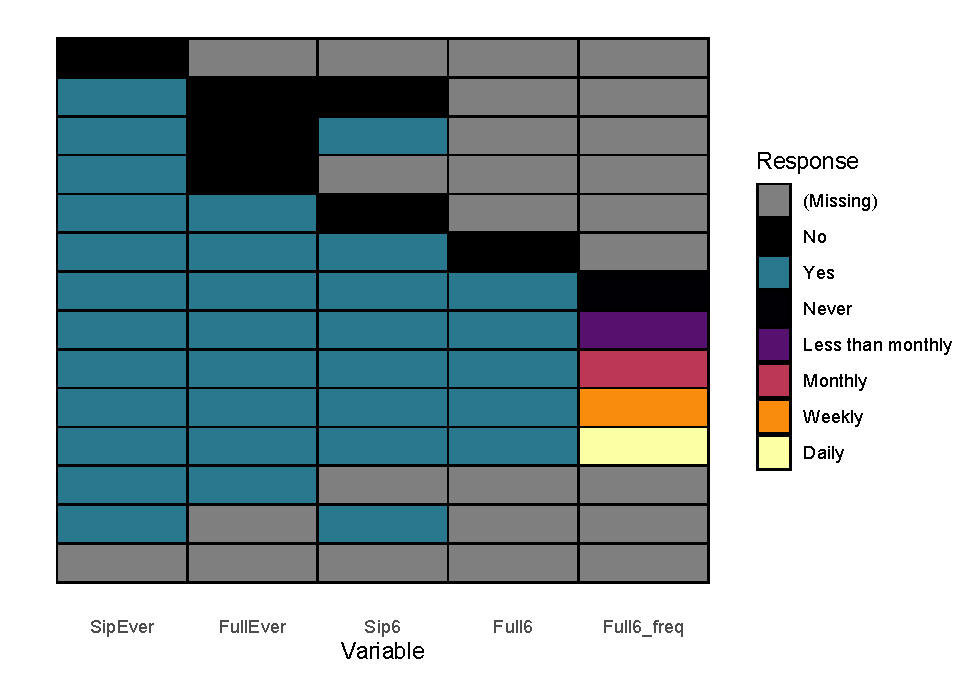
\includegraphics{Rad_files/figure-latex/alc_logic_plot-1.pdf}

To get the same kind of overview in table form, you can also use \texttt{count()}:

\begin{Shaded}
\begin{Highlighting}[]
\FunctionTok{count}\NormalTok{(real, SipEver, FullEver, Sip6, Full6, Full6\_freq)}
\end{Highlighting}
\end{Shaded}

\begin{verbatim}
## # A tibble: 14 x 6
##    SipEver FullEver Sip6  Full6 Full6_freq            n
##    <fct>   <fct>    <fct> <fct> <fct>             <int>
##  1 No      <NA>     <NA>  <NA>  <NA>                523
##  2 Yes     No       No    <NA>  <NA>                394
##  3 Yes     No       Yes   <NA>  <NA>                376
##  4 Yes     No       <NA>  <NA>  <NA>                 16
##  5 Yes     Yes      No    <NA>  <NA>                155
##  6 Yes     Yes      Yes   No    <NA>                 11
##  7 Yes     Yes      Yes   Yes   Never                63
##  8 Yes     Yes      Yes   Yes   Less than monthly    11
##  9 Yes     Yes      Yes   Yes   Monthly              10
## 10 Yes     Yes      Yes   Yes   Weekly                1
## 11 Yes     Yes      Yes   Yes   Daily                 2
## 12 Yes     Yes      <NA>  <NA>  <NA>                  4
## 13 Yes     <NA>     Yes   <NA>  <NA>                  2
## 14 <NA>    <NA>     <NA>  <NA>  <NA>                 50
\end{verbatim}

To analyse the data properly, we'll need to fill in the ``No'' responses that
can be assumed (because of the logic of the survey), instead of leaving
them missing.

There's no real trick to this, the hard part is getting a clear picture
of what needs to be done like we did above. As long as we fill in
the variables in order, we should get the right results:

\begin{Shaded}
\begin{Highlighting}[]
\CommentTok{\# If they\textquotesingle{}ve never sipped, they\textquotesingle{}ve never had a full drink}
\CommentTok{\#   and haven\textquotesingle{}t sipped in the past 6 months}
\NormalTok{real}\SpecialCharTok{$}\NormalTok{FullEver[real}\SpecialCharTok{$}\NormalTok{SipEver }\SpecialCharTok{==} \StringTok{"No"}\NormalTok{] }\OtherTok{=} \StringTok{"No"}
\NormalTok{real}\SpecialCharTok{$}\NormalTok{Sip6[real}\SpecialCharTok{$}\NormalTok{SipEver }\SpecialCharTok{==} \StringTok{"No"}\NormalTok{] }\OtherTok{=} \StringTok{"No"}

\CommentTok{\# If they haven\textquotesingle{}t had a full drink ever, they haven\textquotesingle{}t}
\CommentTok{\#   had one in the past 6 months }
\NormalTok{real}\SpecialCharTok{$}\NormalTok{Full6[real}\SpecialCharTok{$}\NormalTok{FullEver }\SpecialCharTok{==} \StringTok{"No"}\NormalTok{] }\OtherTok{=} \StringTok{"No"}

\CommentTok{\# If they haven\textquotesingle{}t had a sip recently, they haven\textquotesingle{}t}
\CommentTok{\#   had a full drink }
\NormalTok{real}\SpecialCharTok{$}\NormalTok{Full6[real}\SpecialCharTok{$}\NormalTok{Sip6 }\SpecialCharTok{==} \StringTok{"No"}\NormalTok{] }\OtherTok{=} \StringTok{"No"}

\CommentTok{\# If they haven\textquotesingle{}t had a full drink, their frequency}
\CommentTok{\#   of drinking is zero}
\NormalTok{real}\SpecialCharTok{$}\NormalTok{Full6\_freq[real}\SpecialCharTok{$}\NormalTok{Full6 }\SpecialCharTok{==} \StringTok{"No"}\NormalTok{] }\OtherTok{=} \StringTok{"Never"}
\end{Highlighting}
\end{Shaded}

If we look at the pattern of responses again we should see that
all the relevant responses have now bene filled in. Where
missing values remain, it's because we can't automatically
assume a response:

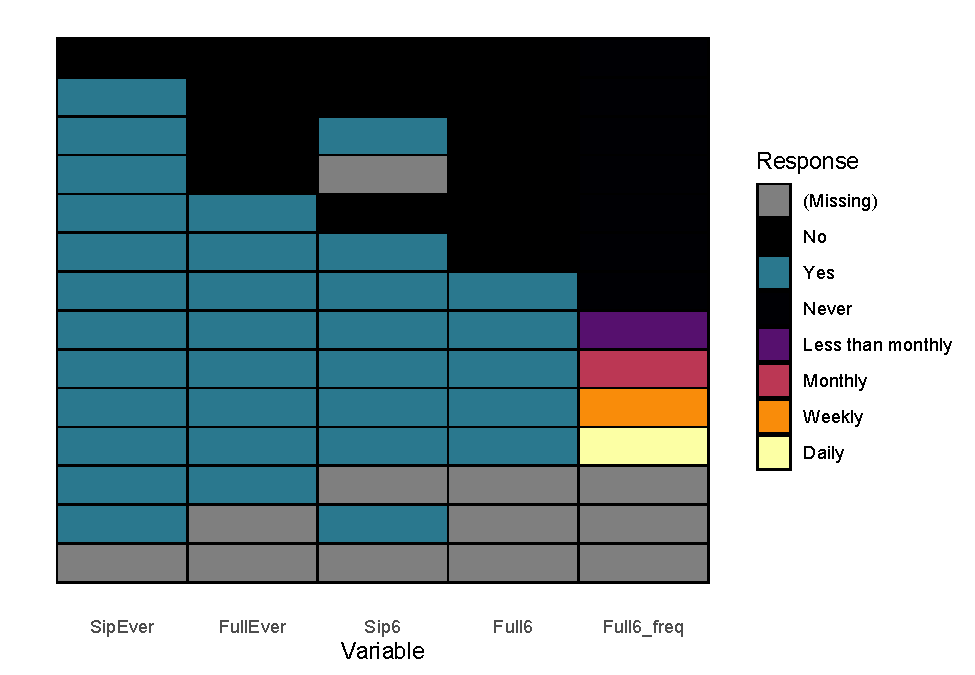
\includegraphics{Rad_files/figure-latex/alc_logic_plot_after-1.pdf}

\hypertarget{saving-data}{%
\section{Saving data}\label{saving-data}}

Now that the data has been recoded and cleaned, we
can save it. R can output to lots of different formats,
so you can choose whichever format works best for you.

However, if you want to keep working in R, it's best
to save it in a format that preserves all the info
about your data, including the order of categories
in your factors. SPSS and Stata formats will do this,
while Excel won't. For now, we'll use R's own
\textbf{.rds} format, which preserves all that information:

\begin{Shaded}
\begin{Highlighting}[]
\NormalTok{readr}\SpecialCharTok{::}\FunctionTok{write\_rds}\NormalTok{(real, }\StringTok{"CapData{-}Recoded.rds"}\NormalTok{)}
\end{Highlighting}
\end{Shaded}

\hypertarget{descriptive-statistics-1}{%
\section{Descriptive statistics}\label{descriptive-statistics-1}}

Once our data has been recoded and cleaned, we can
start looking at descriptive statistics - this
is always a good first step before trying any actual
analysis.

\hypertarget{correlations-between-variables}{%
\subsection{Correlations between variables}\label{correlations-between-variables}}

We can get a good overview of the relationships between
different variables using a \textbf{scatterplot matrix},
which shows correlations between each pair of variables.
\texttt{psych} has a function \texttt{pairs.panel} to handle this:

\begin{Shaded}
\begin{Highlighting}[]
\NormalTok{key\_vars }\OtherTok{=} \FunctionTok{c}\NormalTok{(}\StringTok{"NtTotal\_z"}\NormalTok{, }\StringTok{"AsTotal\_z"}\NormalTok{, }\StringTok{"ImpTotal\_z"}\NormalTok{, }
             \StringTok{"SsTotal\_z"}\NormalTok{, }\StringTok{"DepTotal"}\NormalTok{, }\StringTok{"AnxTotal"}\NormalTok{)}
\NormalTok{psych}\SpecialCharTok{::}\FunctionTok{pairs.panels}\NormalTok{(real[, key\_vars])}
\end{Highlighting}
\end{Shaded}

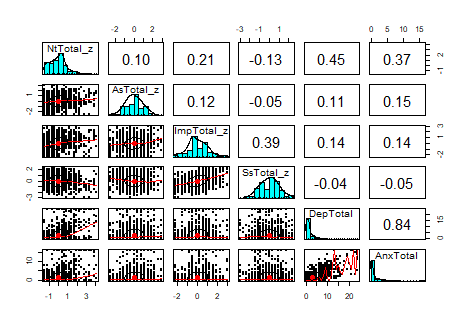
\includegraphics{Rad_files/figure-latex/scatter_matrix_example-1.png}

\begin{note}
Also check out the \texttt{ggcorrplot} package for a nicer-looking
version of this.
\end{note}

If we want a traditional correlation table, we can use
\texttt{psych::corr.test}, which provides both the correlations
between variables and the \emph{p} values for each correlation
coefficient.

\begin{Shaded}
\begin{Highlighting}[]
\NormalTok{psych}\SpecialCharTok{::}\FunctionTok{corr.test}\NormalTok{(real[, key\_vars])}
\end{Highlighting}
\end{Shaded}

\begin{verbatim}
## Call:psych::corr.test(x = real[, key_vars])
## Correlation matrix 
##            NtTotal_z AsTotal_z ImpTotal_z SsTotal_z DepTotal AnxTotal
## NtTotal_z       1.00      0.10       0.21     -0.13     0.45     0.37
## AsTotal_z       0.10      1.00       0.12     -0.05     0.11     0.15
## ImpTotal_z      0.21      0.12       1.00      0.39     0.14     0.14
## SsTotal_z      -0.13     -0.05       0.39      1.00    -0.04    -0.05
## DepTotal        0.45      0.11       0.14     -0.04     1.00     0.84
## AnxTotal        0.37      0.15       0.14     -0.05     0.84     1.00
## Sample Size 
## [1] 1618
## Probability values (Entries above the diagonal are adjusted for multiple tests.) 
##            NtTotal_z AsTotal_z ImpTotal_z SsTotal_z DepTotal AnxTotal
## NtTotal_z          0      0.00          0      0.00     0.00     0.00
## AsTotal_z          0      0.00          0      0.08     0.00     0.00
## ImpTotal_z         0      0.00          0      0.00     0.00     0.00
## SsTotal_z          0      0.03          0      0.00     0.11     0.11
## DepTotal           0      0.00          0      0.09     0.00     0.00
## AnxTotal           0      0.00          0      0.05     0.00     0.00
## 
##  To see confidence intervals of the correlations, print with the short=FALSE option
\end{verbatim}

\hypertarget{contingency-tables-for-categorical-data}{%
\subsection{Contingency tables for categorical data}\label{contingency-tables-for-categorical-data}}

To generate cross-tabs or contigency tables for categorical
variables, we can use \texttt{table()}, which we've already seen
earlier:

\begin{Shaded}
\begin{Highlighting}[]
\FunctionTok{table}\NormalTok{(real}\SpecialCharTok{$}\NormalTok{Group, real}\SpecialCharTok{$}\NormalTok{Sex)}
\end{Highlighting}
\end{Shaded}

\begin{verbatim}
##            
##             Female Male
##   Control      305  423
##   Treatment    386  502
\end{verbatim}

If we want to do some basic testing to see if the
proportions of males and females differ, we can use \texttt{chisq.test()}

\begin{Shaded}
\begin{Highlighting}[]
\FunctionTok{chisq.test}\NormalTok{(real}\SpecialCharTok{$}\NormalTok{Group, real}\SpecialCharTok{$}\NormalTok{Sex)}
\end{Highlighting}
\end{Shaded}

\begin{verbatim}
## 
##  Pearson's Chi-squared test with Yates' continuity correction
## 
## data:  real$Group and real$Sex
## X-squared = 0.34263, df = 1, p-value = 0.5583
\end{verbatim}

If we wanted to visualize these numbers instead,
that's easy to achieve in \texttt{ggplot}:

\begin{Shaded}
\begin{Highlighting}[]
\FunctionTok{ggplot}\NormalTok{(real, }\FunctionTok{aes}\NormalTok{(}\AttributeTok{x =}\NormalTok{ Group, }\AttributeTok{fill =}\NormalTok{ Sex)) }\SpecialCharTok{+}
    \FunctionTok{geom\_bar}\NormalTok{(}\AttributeTok{position =} \StringTok{\textquotesingle{}dodge\textquotesingle{}}\NormalTok{, }\AttributeTok{colour =} \StringTok{\textquotesingle{}black\textquotesingle{}}\NormalTok{)}
\end{Highlighting}
\end{Shaded}

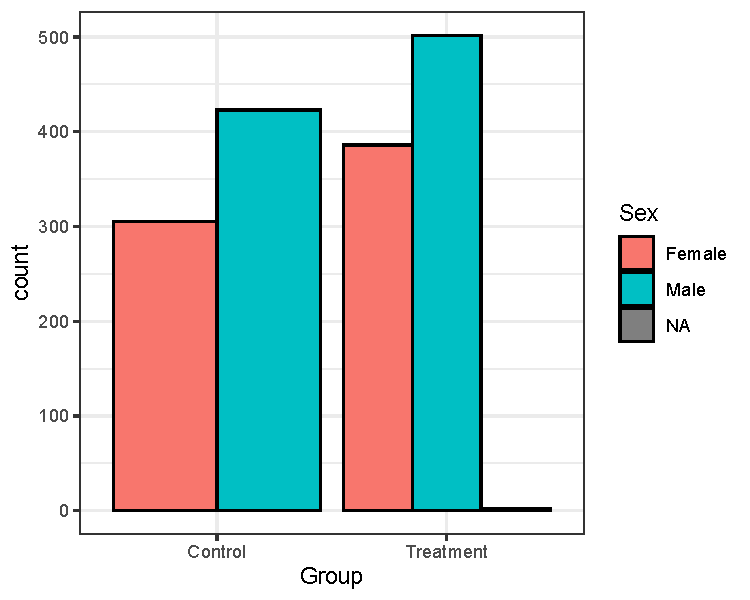
\includegraphics{Rad_files/figure-latex/real_ggplot_bar_example-1.pdf}

\hypertarget{understanding-complex-data}{%
\subsection{Understanding complex data}\label{understanding-complex-data}}

Before trying to do analysis, it can be useful to try
to understand some of the more complex features of your
data. In this study, one important feature is the
cluster randomization, where participants are grouped
in schools - we'll need to account for this in our analysis
so it's worth trying to get a picture of how it looks.

We'll try to look at the means of some variables in each
school. Complex grouped data like this is where the
\texttt{tidyverse} starts to be really useful, so we'll
start making heavy use of it. We'll start by generating
a table:

\begin{Shaded}
\begin{Highlighting}[]
\NormalTok{dep\_tab }\OtherTok{=}\NormalTok{ real }\SpecialCharTok{\%\textgreater{}\%}
  \FunctionTok{group\_by}\NormalTok{(Group, SchoolId) }\SpecialCharTok{\%\textgreater{}\%}
  \FunctionTok{summarize}\NormalTok{(}
    \AttributeTok{DepMean =} \FunctionTok{mean}\NormalTok{(DepTotal, }\AttributeTok{na.rm =} \ConstantTok{TRUE}\NormalTok{),}
    \AttributeTok{SchoolSize =} \FunctionTok{n}\NormalTok{()}
\NormalTok{  )}
\end{Highlighting}
\end{Shaded}

\begin{verbatim}
## `summarise()` has grouped output by 'Group'. You can override using the
## `.groups` argument.
\end{verbatim}

\begin{Shaded}
\begin{Highlighting}[]
\FunctionTok{head}\NormalTok{(dep\_tab)}
\end{Highlighting}
\end{Shaded}

\begin{verbatim}
## # A tibble: 6 x 4
## # Groups:   Group [1]
##   Group   SchoolId DepMean SchoolSize
##   <chr>      <dbl>   <dbl>      <int>
## 1 Control        1    3.03         39
## 2 Control        2    2.72         40
## 3 Control        3    2.48         44
## 4 Control        4    1.17         30
## 5 Control        5    2.84         32
## 6 Control        6    2.12         32
\end{verbatim}

Once we've got this information in a table, it's
easy to create a \texttt{ggplot} plot to visualize it

\begin{Shaded}
\begin{Highlighting}[]
\FunctionTok{ggplot}\NormalTok{(dep\_tab, }\FunctionTok{aes}\NormalTok{(}\AttributeTok{x =}\NormalTok{ Group, }\AttributeTok{y =}\NormalTok{ DepMean, }
                    \AttributeTok{colour =}\NormalTok{ Group)) }\SpecialCharTok{+}
  \FunctionTok{geom\_jitter}\NormalTok{(}\FunctionTok{aes}\NormalTok{(}\AttributeTok{size =}\NormalTok{ SchoolSize), }\AttributeTok{alpha=} \FloatTok{0.5}\NormalTok{,}
              \AttributeTok{width =} \FloatTok{0.1}\NormalTok{, }\AttributeTok{height =} \DecValTok{0}\NormalTok{)}
\end{Highlighting}
\end{Shaded}

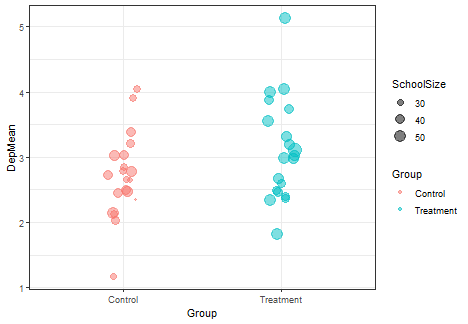
\includegraphics{Rad_files/figure-latex/complex_mean_plot-1.png}

\begin{note}
You can calculate means and summaries within \texttt{ggplot2}, feeding
in your full dataset and using functions like \texttt{stat\_summary()}.
But I'd recommend using \texttt{tidyverse} functions to create a simple
summary table instead,as you'll often run into things \texttt{ggplot}
can't do without a lot of effort.
\end{note}

\hypertarget{analysis-1}{%
\section{Analysis}\label{analysis-1}}

\hypertarget{simple-but-wrong-logistic-regression}{%
\subsection{Simple but wrong: Logistic regression}\label{simple-but-wrong-logistic-regression}}

We'll start with a simple analysis, just comparing
the \textbf{odds} of drinking (a binary outcome) between
the groups. Since this is a binary outcome,
we'll use logistic regression, which is available
in R through the \texttt{glm()} function. This isn't quite
the right approach here, since it doesn't account
for potential correlations between participants in
the same school.

\texttt{glm()} works similarly to \texttt{lm()}, which we saw earlier:
we spell out our model using a formula like \texttt{outcome\ \textasciitilde{}\ predictors}.
For logistic regression we also have to specify
\texttt{family\ =\ binomial(link\ =\ \textquotesingle{}logit\textquotesingle{})}, since that's the distribution
we're using to model the binary outcomes:

\begin{Shaded}
\begin{Highlighting}[]
\NormalTok{simple\_glm }\OtherTok{=} \FunctionTok{glm}\NormalTok{(}
\NormalTok{  Full6 }\SpecialCharTok{\textasciitilde{}}\NormalTok{ Group,}
  \AttributeTok{data =}\NormalTok{ real,}
  \AttributeTok{family =} \FunctionTok{binomial}\NormalTok{(}\AttributeTok{link =} \StringTok{"logit"}\NormalTok{)}
\NormalTok{)}

\FunctionTok{summary}\NormalTok{(simple\_glm)}
\end{Highlighting}
\end{Shaded}

\begin{verbatim}
## 
## Call:
## glm(formula = Full6 ~ Group, family = binomial(link = "logit"), 
##     data = real)
## 
## Deviance Residuals: 
##     Min       1Q   Median       3Q      Max  
## -0.3595  -0.3595  -0.3197  -0.3197   2.4492  
## 
## Coefficients:
##                Estimate Std. Error z value Pr(>|z|)    
## (Intercept)     -2.7066     0.1540 -17.579   <2e-16 ***
## GroupTreatment  -0.2416     0.2208  -1.094    0.274    
## ---
## Signif. codes:  0 '***' 0.001 '**' 0.01 '*' 0.05 '.' 0.1 ' ' 1
## 
## (Dispersion parameter for binomial family taken to be 1)
## 
##     Null deviance: 671.54  on 1561  degrees of freedom
## Residual deviance: 670.34  on 1560  degrees of freedom
##   (56 observations deleted due to missingness)
## AIC: 674.34
## 
## Number of Fisher Scoring iterations: 5
\end{verbatim}

\hypertarget{better-output-with-tab_model}{%
\subsubsection*{\texorpdfstring{Better output with \texttt{tab\_model()}}{Better output with tab\_model()}}\label{better-output-with-tab_model}}
\addcontentsline{toc}{subsubsection}{Better output with \texttt{tab\_model()}}

While \texttt{summary()} gives us lots of useful info about
the model, it's not particularly readable or nice looking.
We'll use \texttt{tab\_model()} for nicer output:

\begin{Shaded}
\begin{Highlighting}[]
\FunctionTok{tab\_model}\NormalTok{(simple\_glm)}
\end{Highlighting}
\end{Shaded}

~

Full 6

Predictors

Odds Ratios

CI

p

(Intercept)

0.07

0.05~--~0.09

\textless0.001

Group {[}Treatment{]}

0.79

0.51~--~1.21

0.274

Observations

1562

R2 Tjur

0.001

\hypertarget{visualizing-our-model-with-plot_model}{%
\subsubsection*{\texorpdfstring{Visualizing our model with \texttt{plot\_model()}}{Visualizing our model with plot\_model()}}\label{visualizing-our-model-with-plot_model}}
\addcontentsline{toc}{subsubsection}{Visualizing our model with \texttt{plot\_model()}}

It can be difficult to understand how logistic
regression relates to the actual probability
of the outcome. Thankfully \texttt{plot\_model()} can
automatically convert the intervention
effect in the model to \textbf{predicted probabilities}:

\begin{Shaded}
\begin{Highlighting}[]
\FunctionTok{plot\_model}\NormalTok{(simple\_glm,}
           \AttributeTok{type =} \StringTok{"pred"}\NormalTok{,}
           \AttributeTok{terms =} \StringTok{"Group"}\NormalTok{)}
\end{Highlighting}
\end{Shaded}

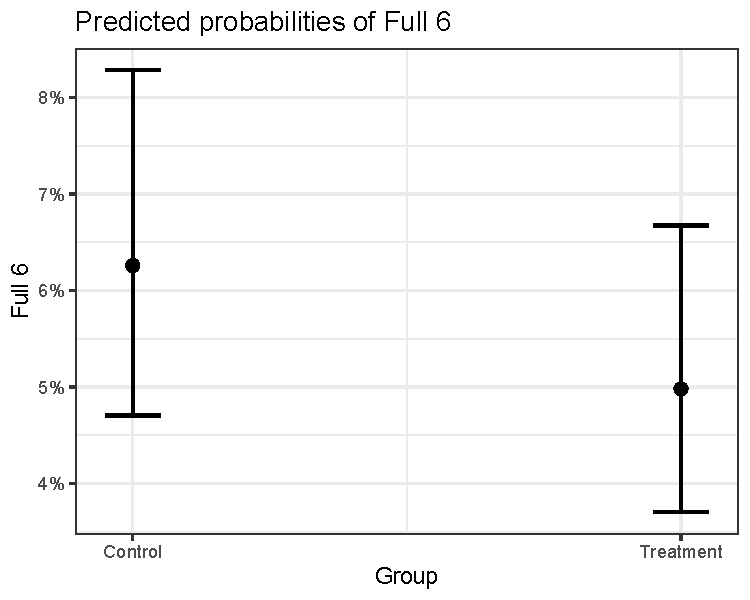
\includegraphics{Rad_files/figure-latex/simple_glm_plot_model-1.pdf}

\hypertarget{more-complex-modelling-mixed-models-with-lme4}{%
\subsection{\texorpdfstring{More complex modelling: Mixed models with \texttt{lme4}}{More complex modelling: Mixed models with lme4}}\label{more-complex-modelling-mixed-models-with-lme4}}

To account for the clustering in the data,
we'll use a \textbf{mixed model} from the \texttt{lme4}
package. Adapting our model from above to
the mixed model approach doesn't require
many changes, since the models use basically
the \textbf{same syntax} and we can use some
of the same \textbf{reporting and visualization
tools} to help interpret them.

Instead of the \texttt{glm()} function, we'll use \texttt{glmer()}
from the \texttt{lme4} package. To add \textbf{random intercepts}
for each school into the model, we just need to tweak
the syntax slightly:

\begin{Shaded}
\begin{Highlighting}[]
\NormalTok{mixed\_glm }\OtherTok{=} \FunctionTok{glmer}\NormalTok{(}
\NormalTok{  Full6 }\SpecialCharTok{\textasciitilde{}}\NormalTok{ Group }\SpecialCharTok{+}\NormalTok{ (}\DecValTok{1} \SpecialCharTok{|}\NormalTok{ SchoolId),}
  \AttributeTok{data =}\NormalTok{ real,}
  \AttributeTok{family =} \FunctionTok{binomial}\NormalTok{(}\AttributeTok{link =} \StringTok{"logit"}\NormalTok{)}
\NormalTok{)}

\FunctionTok{summary}\NormalTok{(mixed\_glm)}
\end{Highlighting}
\end{Shaded}

\begin{verbatim}
## Generalized linear mixed model fit by maximum likelihood (Laplace
##   Approximation) [glmerMod]
##  Family: binomial  ( logit )
## Formula: Full6 ~ Group + (1 | SchoolId)
##    Data: real
## 
##      AIC      BIC   logLik deviance df.resid 
##    676.2    692.3   -335.1    670.2     1559 
## 
## Scaled residuals: 
##     Min      1Q  Median      3Q     Max 
## -0.2702 -0.2548 -0.2367 -0.2254  4.5686 
## 
## Random effects:
##  Groups   Name        Variance Std.Dev.
##  SchoolId (Intercept) 0.02679  0.1637  
## Number of obs: 1562, groups:  SchoolId, 20
## 
## Fixed effects:
##                Estimate Std. Error z value Pr(>|z|)    
## (Intercept)     -2.7200     0.1637 -16.616   <2e-16 ***
## GroupTreatment  -0.2414     0.2210  -1.092    0.275    
## ---
## Signif. codes:  0 '***' 0.001 '**' 0.01 '*' 0.05 '.' 0.1 ' ' 1
## 
## Correlation of Fixed Effects:
##             (Intr)
## GroupTrtmnt -0.657
\end{verbatim}

\hypertarget{using-tab_model-again}{%
\subsubsection{\texorpdfstring{Using \texttt{tab\_model()} again}{Using tab\_model() again}}\label{using-tab_model-again}}

\begin{Shaded}
\begin{Highlighting}[]
\FunctionTok{tab\_model}\NormalTok{(mixed\_glm)}
\end{Highlighting}
\end{Shaded}

~

Full 6

Predictors

Odds Ratios

CI

p

(Intercept)

0.07

0.05~--~0.09

\textless0.001

Group {[}Treatment{]}

0.79

0.51~--~1.21

0.275

Random Effects

σ2

3.29

τ00 SchoolId

0.03

ICC

0.01

N SchoolId

20

Observations

1562

Marginal R2 / Conditional R2

0.004 / 0.012

\hypertarget{and-plot_model-again}{%
\subsubsection{\texorpdfstring{And \texttt{plot\_model()} again}{And plot\_model() again}}\label{and-plot_model-again}}

\begin{Shaded}
\begin{Highlighting}[]
\FunctionTok{plot\_model}\NormalTok{(mixed\_glm,}
           \AttributeTok{type =} \StringTok{\textquotesingle{}pred\textquotesingle{}}\NormalTok{,}
           \AttributeTok{terms =} \StringTok{\textquotesingle{}Group\textquotesingle{}}\NormalTok{)}
\end{Highlighting}
\end{Shaded}

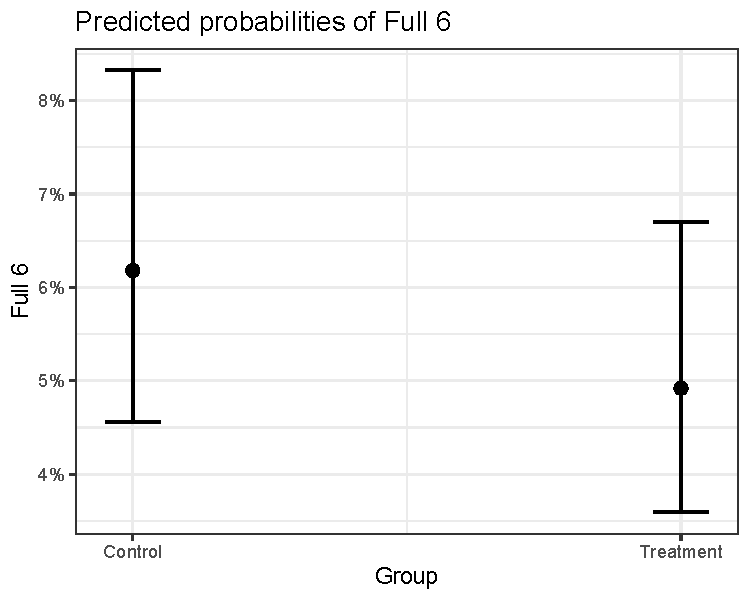
\includegraphics{Rad_files/figure-latex/glmer_plot_model-1.pdf}

\hypertarget{learning-moregetting-help}{%
\chapter*{Learning more/Getting help}\label{learning-moregetting-help}}
\addcontentsline{toc}{chapter}{Learning more/Getting help}

\hypertarget{more-coursesbooks}{%
\section*{More courses/books}\label{more-coursesbooks}}
\addcontentsline{toc}{section}{More courses/books}

If you want more material than is covered in this course,
there are lots of different introductions to R out there,
many of them free.

My number one recommendation is the book \href{https://r4ds.had.co.nz/}{R for Data Science},
written by Garrett Grolemund and Hadley Wickham (who we met at the start of
the course). It's a comprehensive and accessible intro that covers visualization,
data wrangling and analysis, all using modern R tools to make things as easy as possible.

\begin{figure}
\centering
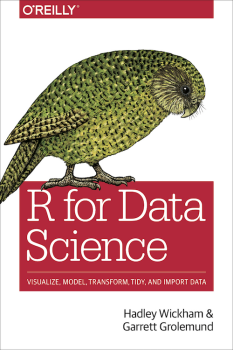
\includegraphics{Images/r4ds.png}
\caption{R for Data Science}
\end{figure}

Other good resources include:

\begin{itemize}
\tightlist
\item
  \href{https://swirlstats.com/}{swirl}, an interactive tutorial for R.
\item
  The \href{https://www.r-graph-gallery.com/}{R Graph Gallery}: lots of cool examples of
  different plots.
\item
  The \href{https://r-graphics.org/}{R Graphics Cookbook}, which has a huge number
  of examples of useful plots, mostly in \texttt{ggplot2}.
\item
  Any of the other books listed on \href{https://bookdown.org/}{bookdown.org}.
\item
  The R courses on \href{https://www.datacamp.com/}{DataCamp}, which have a cool
  interactive system that tests you as you go. Most are paid but there are free trials
  to test it out.
\end{itemize}

\hypertarget{checking-out-the-r-community}{%
\section*{Checking out the R community}\label{checking-out-the-r-community}}
\addcontentsline{toc}{section}{Checking out the R community}

\begin{itemize}
\tightlist
\item
  If you're on Twitter, check out the \href{https://twitter.com/hashtag/rstats}{\#rstats}
  hashtag.
\item
  Check out \href{https://www.r-bloggers.com/}{R Bloggers}, which collects blog posts
  from a huge number of different R blogs.
\end{itemize}

\hypertarget{getting-help}{%
\section*{Getting help}\label{getting-help}}
\addcontentsline{toc}{section}{Getting help}

If you're stuck with your R code, the best option is to \textbf{ask someone you know
who knows R} - some problems can be solved very quickly with a nudge in
the right direction from someone who's experienced them before.

\href{https://stackoverflow.com/}{Stack Overflow} is a resource used by programmers
the world over. Lots of experienced programmers are happy to answer questions
on there to keep their skills sharp and earn useless points
(I have \href{https://stackoverflow.com/users/1222578/marius}{a lot of these useless points}).
The trick to asking a question on Stack Overflow is:

\begin{itemize}
\tightlist
\item
  Do a few google searches for your question before heading to Stack Overflow. The
  answer you need might pop up (and will often already be on Stack Overflow).
\item
  Carefully read the guide to creating a
  \href{https://stackoverflow.com/questions/5963269/how-to-make-a-great-r-reproducible-example}{reproducible example}
  for your question.
\item
  Try to write a question that includes both the code you're already tried, and a
  copy-pasteable version of your dataset.
\end{itemize}

Stack Overflow works best for small, self-contained coding questions, with an objective
answer. If you have a broader question that involves a bit more opinion,
you may want to try on the \href{https://community.rstudio.com/}{RStudio Community forum}.

\hypertarget{why-r-is-good}{%
\chapter*{Why R is Good}\label{why-r-is-good}}
\addcontentsline{toc}{chapter}{Why R is Good}

I've tried to keep the actual material in this course focussed on actually
teaching R. Here, I'll make a brief attempt at evangelizing for R, and
outline why I think it's better than other stats-focussed tools
like SPSS and Stata.

\hypertarget{r-is-a-language}{%
\section*{R is a Language}\label{r-is-a-language}}
\addcontentsline{toc}{section}{R is a Language}

R is not just a program that you issue commands to - it's a language with
consistent rules you can learn, and all the tools in R are written using that
language and those rules\footnote{The exception to this is that the most basic components
  of R, like addition of numbers, are written in C for speed. These are
  usually the components that are so ``low-level'' that you don't need
  to modify them.}. That means:

\begin{itemize}
\tightlist
\item
  Every tool and function you use is built out of the same basic components.
\item
  You can write tools and functions that are just as capable and flexible
  as the built-in tools.
\item
  If you need to, you can ``open up'' other people's tools and change,
  modify or improve them.
\end{itemize}

\hypertarget{r-is-a-programming-language}{%
\section*{R is a programming language}\label{r-is-a-programming-language}}
\addcontentsline{toc}{section}{R is a programming language}

As well as being a language, R is specifically a \emph{programming} language, and
has some of the standard features of programming languages that allow them
to be flexible, and to ``abstract away'' the low-level details of tasks so you\\
can concentrate on the bigger picture.

Every part of your data in R is available as an R object, and you can
access, modify and change it the same way as any other data.
For example, you can get the column names of your data set as a
character vector, which then works the same way as a text column
in your actual data. Then you can:

\begin{itemize}
\tightlist
\item
  Use some code to select a subset of your columns (without typing them
  all out manually)
\item
  Write code that will automatically apply the same recoding step to each
  of those columns (by ``looping'' or ``iterating'') over them.
\item
  Write a function that can carry out these same steps on a brand
  new dataset with completely different column names.
\end{itemize}

\hypertarget{r-has-an-active-community}{%
\section*{R has an active community}\label{r-has-an-active-community}}
\addcontentsline{toc}{section}{R has an active community}

There's a huge wealth of information about R available on the internet,
thanks to the fact that people are constantly working on it, discussing it,
and making their work public. That means getting help with R is often much
easier than in other languages, where it seems like the same 4 academics
have been (condescendingly) answering questions for years.

  \bibliography{book.bib}

\end{document}
